\documentclass{article}%
\usepackage{pbox}
\usepackage{graphicx}
\usepackage{amsmath}
\usepackage{amssymb}
\usepackage{subfigure}
\usepackage{verbatim}
\usepackage[font={small,it}]{caption}
\usepackage{epstopdf}
%\usepackage[colorlinks=true]{hyperref}
\usepackage[affil-it]{authblk}
\usepackage{float}
\usepackage{color}
\usepackage{amsfonts}
\usepackage[margin=1in]{geometry}%
\setcounter{MaxMatrixCols}{30}
\usepackage[title]{appendix}

\newcommand{\highred}[1]{{\color{red}#1}}
\newcommand{\highblue}[1]{{\color{blue}#1}}
\newcommand{\highgreen}[1]{{\color{green}#1}}

\def\ni{\noindent}
\def\proof{{\ni \bf \underline{Proof:} }}
\def\endproof{\hfill$\blacksquare$\vspace{6pt}}

\newtheorem{theorem}{Theorem}[section]
\newtheorem{lemma}[theorem]{Lemma}
\newtheorem{mainres}[theorem]{Main Result}
\newtheorem{lem}[theorem]{Lemma}
\newtheorem{rem}[theorem]{Remark}
\newtheorem{thm}[theorem]{Theorem}
\newtheorem{conj}[theorem]{Conjecture}
\newtheorem{openq}[theorem]{Open question}
\newtheorem{prop}[theorem]{Proposition}
\newtheorem{proposition}[theorem]{Proposition}
\newtheorem{cor}[theorem]{Corollary}
\newtheorem{fact}[theorem]{Fact}
\newtheorem{resu}{Principal Result}[section]

\renewcommand\thesection{\arabic{section}}
\renewcommand\thesubsection{\thesection.\arabic{subsection}}
\renewcommand\thesubsubsection{\thesubsection.\arabic{subsubsection}}
\renewcommand\theequation{\thesection.\arabic{equation}}
\renewcommand{\eqref}[1]{(\ref{#1})}
\usepackage[numbers,sort&compress]{natbib}


\textwidth=7.4in
\hoffset=-0.4in
\textheight=9.0in

\newenvironment{lyxlist}[1]
{\begin{list}{}
{\settowidth{\labelwidth}{#1}
 \setlength{\leftmargin}{\labelwidth}
 \addtolength{\leftmargin}{\labelsep}
 \renewcommand{\makelabel}[1]{##1\hfil}}}
{\end{list}}
\newenvironment{lyxcode}
{\par\begin{list}{}{
\setlength{\rightmargin}{\leftmargin}
\setlength{\listparindent}{0pt}% needed for AMS classes
\raggedright
\setlength{\itemsep}{0pt}
\setlength{\parsep}{0pt}
\normalfont\ttfamily}%
 \item[]}
{\end{list}}

\newcommand{\eps}{{\displaystyle \varepsilon}}
\newcommand{\lam}{{\displaystyle \lambda}}

\DeclareMathOperator{\sech}{sech}
\newcommand{\eproof}{\; \Box }
\newcommand{\abuv}[2]{\genfrac{}{}{0pt}{}{#1}{#2}}
\newcommand{\bsub}{\begin{subequations}}
\newcommand{\esub}{\end{subequations}$\!$}
\renewcommand{\theequation}{\arabic{section}.\arabic{equation}}
\renewcommand{\thesection}{\arabic{section}}

\newcommand{\dzjp}{D^{+}_{0,j}}
\newcommand{\dzjm}{D^{-}_{0,j}}
\newcommand{\dustar}{D_{\textrm{up}}^{\star}}
\newcommand{\dlstar}{D_{\textrm{low}}^{\star}}

\begin{document}

\title{Asynchronous Instabilities of Crime Hotspots for a 1-D
  Reaction-Diffusion Model of Urban Crime with Focused Police Patrol}
\date{\today} \author{Wang Hung Tse\thanks{Dept. of Mathematics, UBC,
    Vancouver, Canada} \enspace, Michael J. Ward\thanks{Dept. of
    Mathematics, UBC, Vancouver, Canada. (corresponding author {\tt
      ward@math.ubc.ca})}}
\baselineskip=16pt

\maketitle

\begin{abstract}
\highblue{To be written}
\end{abstract}

{\bf Key Words}: Urban crime, hotspot patterns, nonlocal eigenvalue
problem (NLEP), Hopf bifurcation, asynchronous oscillatory
instability, cops-on-the-dots.

\setcounter{equation}{0}
\setcounter{section}{0}
\section{Introduction}\label{sec:intro}

The development of mathematical approaches to quantify and predict
spatial patterns of urban crime originates from the pioneering studies
in \cite{s_1, s_2, s_3}. A primary motivation for this effort is the
increased availability of residential burglary data, which clearly
show that spatial patterns of urban crime are often concentrated in
certain spatial regions, known as hotspots \cite{bb}. It is believed
that these hotspots are due to a repeat or near-repeat victimization
effect, which suggests that crime in a certain region induces more
crime in that and nearby regions (cf.~\cite{jb}, \cite{wk}).

\highblue{Need a small paragraph here about police and general goal: Refer to
  \cite{jbc}, \cite{pitcher}, \cite{zipkin}, \cite{rick}, \cite{smith}
  (agent-based) for different police models.}

% For law enforcement, a seemingly obvious response to a hot spot of
% crime is to deploy additional resources to the hot spot to deter
% further crime. These so-called \cops on the% dots" strategies have
% sometimes successfully dispersed the hot spot, but other times have
% merely displaced the crime to surrounding areas \cite{braga}.

%A disadvantage of the random walk strategy is then clear: the spacial
%distribution of police will become nearly uniform in the long run, and
%hence does not give enough protection to vulnerable locations.
%We observe that this strategy does not reduce hotspot activity, which
%is in consistent with the empirical evidences in \cite{jbc}

%The second mode alters the environment: proximity of police will tend
%to make the local environment less attractive to the criminal
%elements. Hence by reducing the attractiveness value in accord with
%the presence of police agents, there will be a diminished rate of
%criminal activity and a tendency for criminals to move away from
%regions with a high concentration of police agents.

%One possibility is for law enforcement agents to patrol random
%routes. Here police do not focus their attention on any particular
%place. The hope is that criminal activity will be reduced, as the
%criminal agents will never know when an enforcement agent will be
%near. This method has been tried, without much success, in Kansas
%City. The random patrol method has an obvious downside: enforcement
%agents will often be located in places where the level of criminal
%activity is already low.

%In this scheme the law enforcement agents move randomly but with a
%bias in the direction of high attractiveness. We will call this method
%of policing cops on the dots. Similarly, in our model the law
%enforcement agents will tend to patrol areas with relatively high
%attractiveness  areas correlated with a high number of
%individual burglary events. As we will see, cops on the dots is
%effective in reducing criminal activity. In the model, criminal agents
%tend to move from areas of low attractiveness to places where it is
%higher.

%Law enforcement agents patrol areas with high attractiveness which
%reduces the likelihood that criminal agents will commit crimes in these areas
%(and, in the perception modi¯cation model, biases them toward
%locations with lower attractiveness  places where they are less
%likely to commit crime). A criminal agent in this situation is more
%likely to return home without having performed any criminal
%activity. The overall e®ect is that the global statistical rate of
%burglary is lowered.  


%The elimination of crime hotspots may have another unfortunate side
%effect: while crime is reduced in the areas with the highest criminal
%activity it may actually be increased in areas where the criminal
%activity is lower. Displacement of crime has been one outcome observed
%in field-based tests of hotspot policing.49 If criminal agents are
%spending more time outside the center of a crime hotspot, they will be
%more likely to commit crimes in low crime areas.  

Following \cite{rick}, our simple police interaction model on the
one-dimensional domain $0\leq x \leq S$ is formulated as
\bsub\label{eq:crs-main}
\begin{alignat}{1}
A_{t} & =\epsilon^{2}A_{xx}-A+\rho A+\alpha\,, \label{eq:crs-main-A}\\
\rho_{t} & =D\left(\rho_{x}-2\rho A_{x}/A\right)_{x}-\rho A +\gamma-\alpha-
U\,, \label{eq:crs-main-rho}\\
\tau_{u}U_{t} & =D\left(U_{x}-qUA_{x}/A\right)_{x}\,,  \label{eq:crs-main-U}
\end{alignat}
\esub where $A_x=\rho_x=U_x=0$ at $x=0,S$. Here $A$ is the
attractiveness field, while $\rho$ and $U$ are the density of
criminals and police, respectively.  The constants $\alpha$ and
$\gamma-\alpha$ are the baseline attractiveness and the rate at which
new criminals are introduced, respectively. From
(\ref{eq:crs-main-U}), we obtain that the total level $U_0$ of police
deployment is conserved in time, so that
\begin{equation}\label{ss:pol_con}
   U_0 \equiv \int_{0}^{S} U(x,t)\, dx \,.
\end{equation}
In (\ref{eq:crs-main-U}), the parameter $q>0$ measures the degree of
focus in the police patrol toward maxima of the attractiveness field
$A$.  We will assume in our analysis below that $q>1$.  The choice
$q=2$ models a ``cops-on-the-dots'' strategy (cf.~\cite{jbc},
\cite{rick}, \cite{zipkin}) whereby the police have the same degree of
focus as do the criminals towards maxima of $A$. When $q$ is above or
below $2$, the police force drift in a less or more focused manner,
respectively, as compared to that of the criminals. In
(\ref{eq:crs-main}) the constant diffusivities of the criminals and
the police is $D$ and $D_p\equiv {D/\tau_{u}}$, respectively.  The
police are more mobile than the criminals when $\tau_u<1$, while when
$\tau_{u}>1$ the police are comparatively more ``sluggish'' in their
movements.

The corresponding two-component system, where $U_0=0$ and
(\ref{eq:crs-main-U}) is omitted, which we refer to as the {\em basic
  crime model}, was derived in \cite{s_1} and \cite{s_3} from the
continuum limit of an agent-based model that accounts for the effect
of repeat or near-repeat victimization. This two-component RD system
has been well-studied. When $D={\mathcal O}(1)$, a formal weakly
nonlinear analysis was developed in \cite{s_2} to study the
development of small amplitude spatial patterns of crime near a Turing
bifurcation point associated with a spatially homogeneous steady-state
solution. In \cite{ccm} this local branching behavior near the Turing
point was characterized rigorously (see also \cite{GWY}). In \cite{rb}
the local existence of solutions to the basic crime model in
multi-dimensional domains was established.  On the infinite line, and
with $D=1$, an intricate snaking-type bifurcation structure of hotspot
equilibria was computed numerically in \cite{lf} in the singular limit
$\epsilon\to 0$, for the subcritical regime
$\alpha<\gamma<\gamma_c\sim {3\alpha/2}$. On a finite domain with
$D={\mathcal O}(1)$, and for $\gamma>{3\alpha/2}$, in \cite{tw} the
slow dynamics of hotspot quasi-equilibria, together with a nucleation
process through which new hotspots can be created, was revealed. For
the parameter regime $D\gg 1$, hotspot equilibria and their linear
stability properties were analyzed in \cite{kww_crime}. The existence
of these hotspot equilibria for the regime $D\gg 1$ was established
rigorously in \cite{bww} by using a Lyapunov-Schmidt reduction.

Following \cite{kww_crime} for the basic crime model, we will analyze
the three-component system (\ref{eq:crs-main}) for $\epsilon\to 0$
when $D={\mathcal O}(\epsilon^{-2})$. On the $D={\mathcal
  O}(\epsilon^{-2})$ regime, steady-state hotspot patterns for the
basic crime model have a stability threshold \cite{kww_crime}.  Since
$A={\mathcal O}(\epsilon^{-1})$ in a hotspot region, it is convenient,
as in \cite{kww_crime}, to introduce the new variables $v$ and $u$ by
\begin{equation}\label{ss:new_var}
\rho=\epsilon^2 v A^{2}\,, \qquad U=uA^{q} \,, \qquad  
D= \epsilon^{-2} {\mathcal D}_{0} \,.
\end{equation}
In terms of $v$, $u$, and ${\mathcal D}_0={\mathcal O}(1)$,
(\ref{eq:crs-main}) becomes 
\bsub\label{eq:pol-main}
\begin{align}
A_{t} & =\epsilon^{2}A_{xx}-A+\epsilon^{2}vA^{3}+\alpha\,,
 \label{eq:pol-main-A}\\
\epsilon^{2}\left(A^{2}v\right)_{t} & ={\mathcal D}_{0}\left(A^{2}v_{x}\right)_{x}
-\epsilon^{2}vA^{3}+\gamma-\alpha-uA^{q}\,, \label{eq:pol-main-v}\\ 
\tau_{u}\epsilon^{2}\left(A^{q}u\right)_{t}
& ={\mathcal D}_{0}\left(A^{q}u_{x}\right)_{x} \,. \label{eq:pol-main-u}
\end{align}
\esub 

In the limit $\epsilon\to 0$, we will analyze the existence and
linear stability of hotspot steady-state solutions to
(\ref{eq:pol-main}), in which the attractiveness field is spatially
localized. We will construct phase diagrams in parameter space where
such patterns are linearly stable, and show these regions of stability
depend on the parameters $q$, $U_0$, and $D_p$ (or equivalently
$\tau_u$).

For $\epsilon\ll 1$, in \S \ref{sec:pol-construction} we use the
method of matched asymptotic expansions to construct hotspot
steady-state solutions to (\ref{eq:pol-main}) that have a common
hotspot amplitude. In Proposition \ref{thm:
  pol-symm-K-hotspots-for-main} below, we show that such patterns exist for
(\ref{eq:crs-main}) only when $U_0<U_{0,\max}\equiv S(\gamma-\alpha)$
For $q>1$, Proposition \ref{thm: pol-symm-K-hotspots-for-main} also shows
that the total police deployment $U_0$ has an indirect effect on
crime, in that it reduces the maxima, referred to here as
``amplitudes'', of the attractiveness field $A$.

To analyze the linear stability of a $K$-hotspot steady-state
solution, in \S \ref{sec:nlep_deriv} we use asymptotic analysis to
derive the nonlocal eigenvalue problem (NLEP), characterizing
${\mathcal O}(1)$ time-scale instabilities of the pattern. The
methodology to derive this NLEP involves using a reference domain
$|x|\leq \ell$ containing a single hotspot centered at $x=0$, and
then imposing Floquet-type boundary conditions at $x=\pm \ell$.  In
terms of this reference problem, the NLEP for the finite-domain
problem $0<x<S$ with Neumann conditions at $x=0,S$ can then readily be
extracted, as similar to that done in \cite{kww_crime} for the basic
two-component crime model.  Such a Floquet-based approach to study the
linear stability of multi-spike steady-states was first introduced in
\cite{floq-ref} in the context of 1-D spatially-periodic spike patterns
for a class of two-component reaction-diffusion systems. It has
subsequently been extended to study the linear stability of 1-D mesa
patterns \cite{mk_mesa}, of 1-D spikes for a competition model with
cross-diffusion effects \cite{kw_xdiff}, and 1-D hotspot patterns for
the basic crime model \cite{kww_crime}. 

There are two novel features in the derivation of the NLEP for our
three-component RD system. Firstly, in our asymptotic analysis, we
must carefully derive rather intricate jump conditions across the
hotspot region. Secondly, the resulting NLEP that we obtain has two
nonlocal terms, instead of the usual one. As a result, its analysis is
seemingly beyond the general NLEP stability theory with a single
nonlocal term, as surveyed in \cite{wei_rev}.  However, by using a
key identity that is specific to our three-component RD crime
model, we show how to reformulate the NLEP more conveniently in terms
of a single nonlocal term, which can then be more readily analyzed.

Our NLEP linear stability analysis reveals that a steady-state with a
single hotspot is always linearly stable, and that a steady-state with
$K\geq 2$ hotspots is always linearly stable to synchronous
perturbations of the amplitudes of the hotspots.  For $K\geq 2$
hotspots, and for a given $U_0>0$ and fixed $q>1$, our NLEP analysis
provides phase diagrams in the $D_{p}$ versus ${\mathcal D}_0$
parameter plane characterizing the linear stability of the hotspot
steady-states to asynchronous perturbations in the hotspot
amplitudes. For the special case $q=3$, and for $K\geq 2$, for which
the discrete spectrum of the NLEP can be reduced to the study of a
family of $K-1$ quadratic equations in the eigenvalue parameter, these
phase diagrams can be constructed explicitly. Such ``explicitly
solvable'' NLEPs have been analyzed in other contexts
\cite{kww_crime,mtw_enlep,nec}.  For general $q>1$, in \S
\ref{sec:stab_qn3} the phase diagrams are determined by combining some
rigorous spectral results obtained from the argument principle
together with numerical results obtained from a parameterization of
the Hopf bifurcation threshold, as derived from the NLEP. This
analysis shows that steady-state multiple hotspot patterns are
unconditionally unstable if ${\mathcal D}_0>{\mathcal D}_{0,c}$, and
are always linearly stable if $0<{\mathcal D}_0< {\mathcal
  D}_{0,c}/(1+qU_0/\omega)$, where $\omega=S(\gamma-\alpha)-U_0$ and
${\mathcal D}_{0,c}$ is the competition instability threshold given
below in (\ref{stab:zero_d0min}).  Some technical results required for
the analysis of the NLEP, together with a qualitative discussion on how
the competition threshold ${\mathcal D}_{0,c}$ depends on the patrol
focus $q$ and the police deployment are given in \S
\ref{sec:stab_comp}.

\begin{figure}[htbp]
\centering
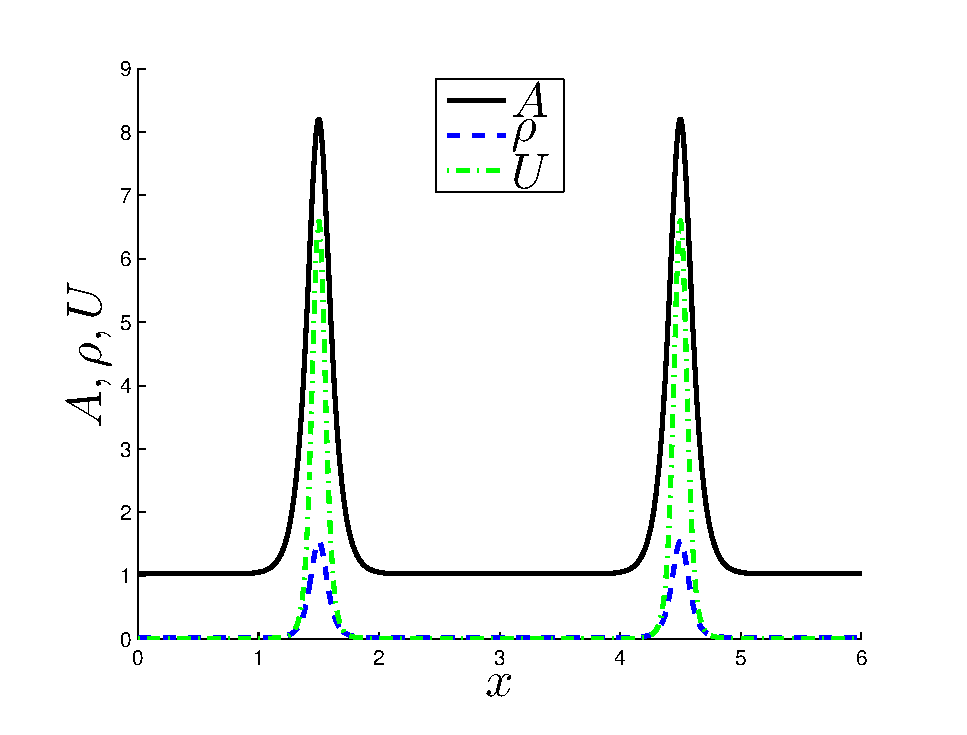
\includegraphics[width=9cm,height=4.8cm]{figs/ss_2_pol_u02.eps}
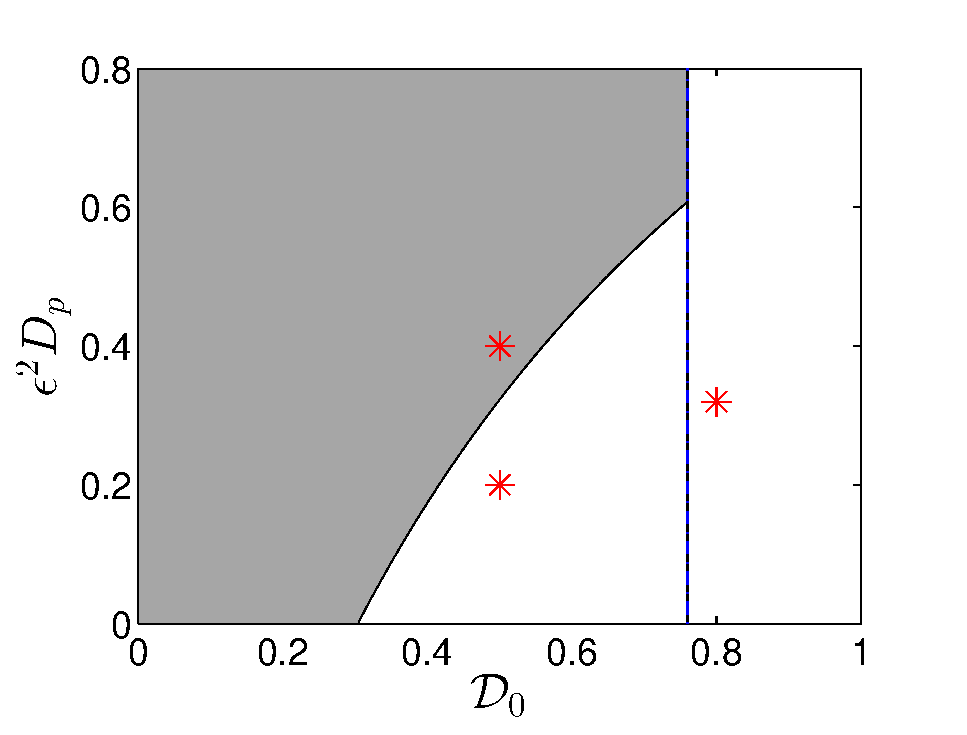
\includegraphics[width=9cm,height=4.8cm]{figs/hopf_2_pol_u02.eps}
\caption{\label{fig:hopf_pol_intro} Left panel: The steady-state
  two-hotspot solution for $S=6$, $\gamma=2$, $\alpha=1$, $U_0=2$,
  ${\mathcal D}_0=0.5$, $\epsilon=0.075$, and $q=3$. Right panel: the
  shaded region of linear stability in the (scaled) police diffusivity
  $\epsilon^{2}D_p\equiv {{\mathcal D}_0/\tau_u}$ versus ${\mathcal
    D}_0$ parameter plane. The thin vertical line is the competition
  stability threshold ${\mathcal D}_{0,c}$ given in Proposition
  \ref{q3:main_twospots}, while the leftmost edge of the instability
  region (at $D_p=0$) is ${{\mathcal D}_{0,c}/(1+{3U_0/\omega})}$
  where $\omega=S(\gamma-\alpha)-U_0$.  For ${\mathcal D}_0>{\mathcal
    D}_{0c}$ the hotspot solution is unstable due to a competition
  instability, while in the unshaded region for ${\mathcal
    D}_0<{\mathcal D}_{0c}$, the hotspot steady-state is unstable to
  an asynchronous oscillatory instability of the hotspot amplitudes. The full
  PDE simulations in Fig.~\ref{fig:valid_2spot_q3} are done at the marked 
  points.}
\end{figure}

On the intermediate range ${\mathcal
  D}_{0,c}/(1+qU_0/\omega)<{\mathcal D}_0<{\mathcal D}_{0,c}$, one of
our main results is that when the police diffusivity $D_p$ dips below
a ${\mathcal D}_0$-dependent threshold, an asynchronous temporal
oscillatory instability in the hotspot amplitudes will occur from a
Hopf bifurcation of the NLEP. These asynchronous, anti-phase,
oscillations of the hotspot amplitudes have the qualitative
interpretation that, at least for short time, the police intervention
has the effect of only displacing crime between different spatial
regions.  Qualitatively, this result is consistent with observations
in \cite{braga} that a ``cops-on-the-dots'' policing strategy will
sometimes not eliminate crime, but instead will only displace it to
surrounding areas. Our full numerical computations of the PDE system
(\ref{eq:pol-main}) suggest that these asynchronous oscillations
arising from the Hopf bifurcation are subcritical, and that over a
longer time-scale they trigger a nonlinear process whereby hotspots
are annihilated.

\begin{figure}[htbp]
\centering
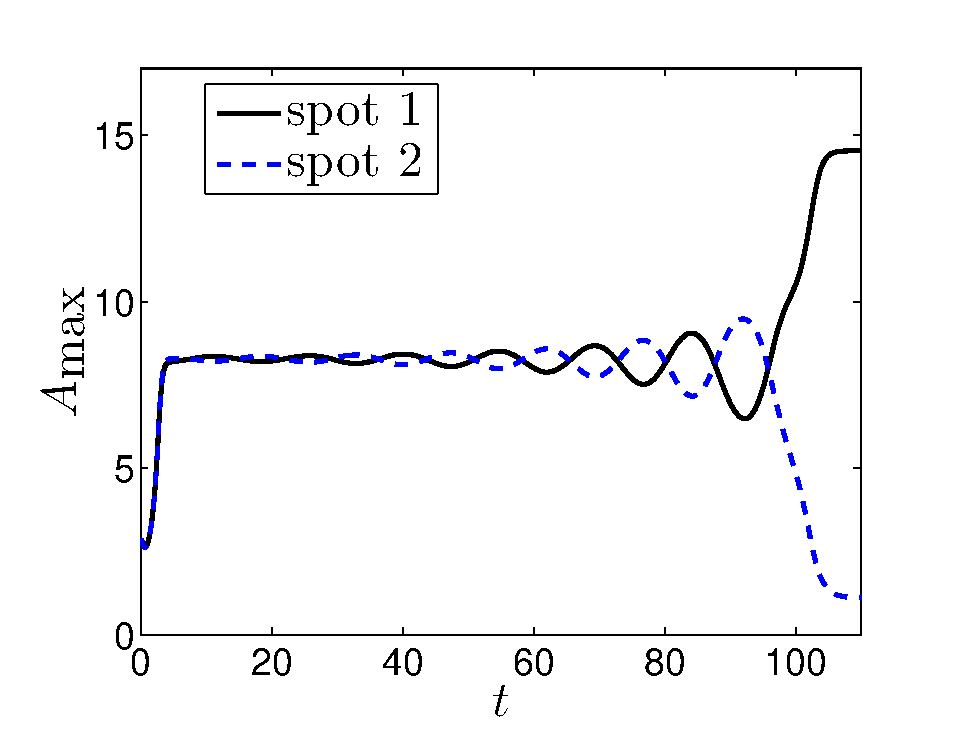
\includegraphics[width=0.32\textwidth,height=4.8cm]{figs/amp_2_run1.eps}
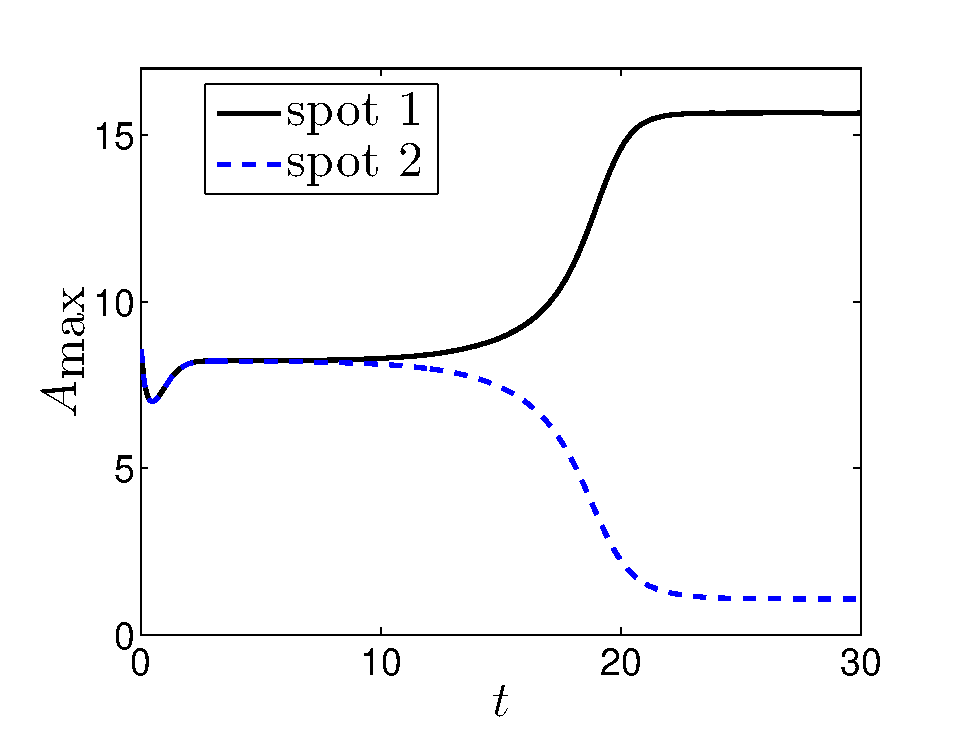
\includegraphics[width=0.32\textwidth,height=4.8cm]{figs/amp_2_run2.eps}
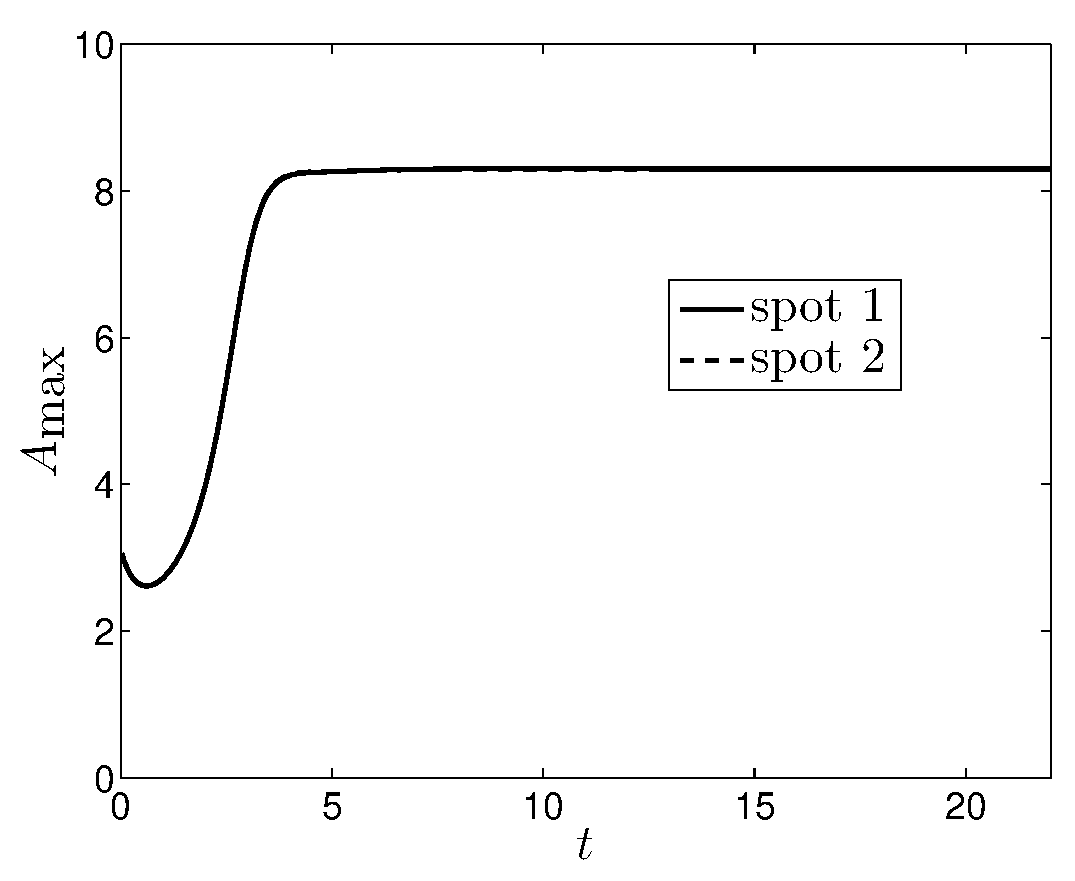
\includegraphics[width=0.32\textwidth,height=4.8cm]{figs/amp_2_run3.eps}
\caption{\label{fig:valid_2spot_q3} Plot of the spot amplitudes
  computed numerically from the full PDE system (\ref{eq:pol-main})
  for a two-spot pattern with $S=6$, $\gamma=2$, $\alpha=1$, $U_0=2$,
  $\epsilon=0.075$, and $q=3$, at the marked points in the right panel of
  Fig.~\ref{fig:hopf_pol_intro}.  Left panel: $\hat{\tau}_u=2.5$ and
  ${\mathcal D}_0=0.5$, so that $\epsilon^2 D_p=0.2$. Spot amplitudes
  are unstable to asynchronous oscillations, which leads to the
  collapse of one hotspot.  Middle panel: $\hat{\tau}_u=2.5$ and
  ${\mathcal D}_0=0.8$, so that $\epsilon^2 D_p=0.32$. Spot amplitudes
  are unstable to a competition instability. Right panel:
  $\hat{\tau}_u=1.25$ and ${\mathcal D}_0=0.5$, so that
  $\epsilon^2D_p=0.4$. Spot amplitudes are stable to asynchronous
  oscillations and there is no competition instability.  These results
  are consistent with the linear stability predictions in the right
  panel of Fig.~\ref{fig:hopf_pol_intro} (see also the left panel of
  Fig.~\ref{fig:hopf_tau_2} below).}
\end{figure}

To illustrate our results, we take $S=6$, $\gamma=2$, $\alpha=1$,
$q=3$, $U_0=2$, and $\epsilon=0.075$, and we consider a steady-state
with exactly two hotspots, as shown in the left panel of
Fig.~\ref{fig:hopf_pol_intro}. For this two-hotspot steady-state the
linear stability phase diagram in the $\epsilon^2 D_p$ versus ${\mathcal D}_0$
parameter plane is shown in the right panel of
Fig.~\ref{fig:hopf_pol_intro}. For the three marked points in the
phase diagram in Fig.~\ref{fig:hopf_pol_intro}, where qualitative
distinct solution behavior occurs, in Fig.~\ref{fig:valid_2spot_q3} we
validate our linear stability predictions by showing full numerical
results for the maxima, or amplitudes, of $A$, as computed from the
PDE system (\ref{eq:pol-main}). The numerical methodology and initial
conditions used in the simulations are discussed in \S
\ref{sec:numerics_q3}. Observe from the left panel in
Fig.~\ref{fig:valid_2spot_q3} that the asynchronous oscillation of the
hotspot amplitudes eventually leads to the annihilation of one of the
two hotspots. Further detailed validations of our linear stability
phase diagrams with full PDE simulations of (\ref{eq:pol-main}) are
given in \S \ref{sec:numerics_q3} for $q=3$ and in \S
\ref{sec:numerics_qn3} for the ``cops-on-the-dots'' policing strategy
$q=2$.

We emphasize that the interval in ${\mathcal D}_0$ for the existence
of asynchronous oscillations vanishes when $U_0=0$. In other words, it
is the third component of the PDE system (\ref{eq:pol-main}), modeling
the police interaction, that is essential for the existence of these
oscillations, with the basic two-component RD crime model
\cite{kww_crime} being incapable of supporting such
oscillations. Robust asynchronous oscillations of localized spikes in
1-D does not occur for many classical two-component RD systems in the
large diffusivity ratio limit, such as the Gray-Scott and
Gierer-Meinhardt models (cf.~\cite{dgk_0}, \cite{iww},
\cite{floq-ref}, \cite{mjww_1}, \cite{kww_gs}). For these
two-component systems, the stability threshold for spike amplitude
oscillations arising from a Hopf bifurcation in the NLEP is set by the
synchronous mode. It is only for more non-traditional RD systems, such
as the 1-D Brusselator model with influx boundary conditions
\cite{tzou} or the Gierer-Meinhardt model with anomalous diffusion
\cite{nec_sub}, that asynchronous oscillations have been shown to be the
dominant oscillatory instability in rather small parameter regimes.

Finally, in \S \ref{sec:disc} we discuss a few open problems motivated
by our study.

\setcounter{equation}{0}
\setcounter{section}{1}
\section{\label{sec:pol-construction}Asymptotic Construction of a Multiple
Hotspot Steady-State}

In this section we construct a steady-state solution to
(\ref{eq:pol-main}) on $0\leq x\leq S$ with $K\geq 1$ interior
hotspots. 

To construct a steady-state with $K$ interior hotspots to
(\ref{eq:pol-main}) on $0<x<S$, where the hotspots have a common
amplitude, we will first construct a one-hotspot solution to
(\ref{eq:pol-main}) on $|x|\leq l$ centered at $x=0$. Then, by using
the translation-invariance property of (\ref{eq:pol-main}), we obtain
a $K$ interior hotspot steady-state solution on the original domain of
length $S=(2\ell)K$. In terms of this reference domain $|x|\leq \ell$,
(\ref{ss:pol_con}) yields that
\begin{equation}
U_{0}=K\int_{-\ell}^{\ell}U\, dx \,. \label{eq:U0-with-K}
\end{equation}
In this way, we need only construct a one-hotspot steady-state
solution to (\ref{eq:pol-main}) centered at $x=0$ and impose
$A_x=v_x=u_x=0$ at $x=\pm \ell$. We refer to this as the {\em
  canonical} hotspot problem.

From the steady-state of (\ref{eq:pol-main-u}), together with
$U=uA^{q}$ and (\ref{eq:U0-with-K}), it follows that $u$ is spatially 
constant and given by
\begin{equation}
u=\frac{U_{0}}{K\int_{-\ell}^{\ell}A^{q}\, dx} \,. \label{eq:pol-u-uniform}
\end{equation}
By using (\ref{eq:pol-u-uniform}) in (\ref{eq:pol-main}), the 
three-component steady-state system reduces to the nonlocal BVP
problem 
\bsub\label{eq:pol-stdy}
\begin{gather}
\epsilon^{2}A_{xx}-A+\epsilon^{2}vA^{3}+\alpha=0\,,\qquad |x|\leq \ell\,;
 \qquad A_x=0 \quad x=\pm \ell \,, \label{eq:pol-stdy-A}\\
{\mathcal D}_{0}\left(A^{2}v_{x}\right)_{x}-\epsilon^{2}vA^{3}+\gamma-\alpha-
\frac{U_{0}}{K}\frac{A^{q}}{\int_{-\ell}^{\ell}A^{q}\, dx}=0\,, \qquad
 |x|\leq \ell\,; \qquad v_x=0 \quad x=\pm \ell \,. \label{eq:pol-stdy-v}
\end{gather}
\esub

We now construct the solution to (\ref{eq:pol-stdy}) with a single
hotspot centered at $x=0$. In the outer region we have
$A\sim\alpha+{\mathcal O}(\epsilon^{2})$, while in the inner region we
put $y=\epsilon^{-1}x$ and $A\sim A_{0}/\epsilon$ to obtain on
$-\infty<y<\infty$ that
\begin{equation*}
A_{0yy}-A_{0}+vA_{0}^{3}+\epsilon\alpha = 0 \,, \qquad
{\mathcal D}_{0}\epsilon^{-4}\left(A_{0}^{2}v_{y}\right)_{y}+{\mathcal
  O}(\epsilon^{-1}) = 0\,.
\end{equation*}
Therefore, to leading order it follows that $v\sim v_{0}$ is a constant,
and that
\begin{equation}
A_{0} \sim \frac{w(y)}{\sqrt{v_{0}}} \,, \label{eq:pol-A-leading}
\end{equation}
where $w(y)=\sqrt{2}\sech y$ is the homoclinic solution of 
\begin{equation}\label{wground}
 w^{\prime\prime}-w+w^{3}=0\,,\qquad-\infty<y<\infty\,; \qquad
w(0)>0\,,\quad w^{\prime}(0)=0\,,\quad w\to0 \quad \mbox{ as }\,\,\, 
y\to\pm\infty\,.
\end{equation}
The integrals of $w(y)$ that are need beelow are
\begin{equation}\label{ss:int} 
 \int_{-\infty}^{\infty}w \, dy=
\int_{-\infty}^{\infty}w^{3} \, dy=\sqrt{2}\pi\,, \quad
\int_{-\infty}^{\infty}w^{2}\,dy=4\,,\quad\int_{-\infty}^{\infty}w^{4}\, dy=
  \frac{16}{3}\,, 
\quad \frac{\int_{-\infty}^{\infty}w^{5}\, dy}{\int_{-\infty}^{\infty}w^{3}\,dy}
 =\frac{3}{2}\,.
\end{equation}
More generally, we can readily calculate in terms of the usual Gamma 
function $\Gamma(z)$ that
\begin{equation}\label{eq:I_q-general-formula}
I_{q}\equiv \int_{-\infty}^{\infty}w^{q}\, dy=
2^{3q/2-1}\frac{\left[\Gamma(q/2)\right]^2}{\Gamma(q)}\,.
\end{equation}

We return to (\ref{eq:pol-u-uniform}), and for $q>1$ we estimate the key 
integral
\[
\int_{-\ell}^{\ell}A^{q}\, dx\sim 2\ell\alpha+\epsilon^{1-q}v_{0}^{-q/2}
\int_{-\infty}^{\infty}w^{q} \, dy= {\mathcal O}(\epsilon^{1-q}) \gg 1 \,.
\]
From (\ref{eq:pol-u-uniform}), we have $u={\mathcal
  O}(\epsilon^{q-1})\ll 1$ since $q>1$.  With our assumption 
$q>1$, the integral $\int_{-\ell}^{\ell}A^{q}\, dx$, and thus $u$, depend
to leading-order only on the inner region contribution from
$A^{q}$. For $q>1$, we obtain to leading-order 
from (\ref{eq:pol-u-uniform}) that 
\begin{equation}
  u\sim\epsilon^{q-1}\tilde{u}_{e}\,, \qquad 
\mbox{where} \qquad \tilde{u}_{e} \equiv
\frac{U_{0} v_{0}^{q/2}}{K I_{q}}\,.\label{eq:pol-u-leading}
\end{equation}

Next, we determine $v_{0}$ by integrating (\ref{eq:pol-stdy-v})
on $-\ell<x<\ell$ and then imposing $v_{x}(\pm\ell)=0$. This yields that
\[
\epsilon^{2}\int_{-\ell}^{\ell}vA^{3}\,dx=
2\ell\left(\gamma-\alpha\right)-U_{0}/K\,.
\]
Therefore, since $A\sim\alpha={\mathcal O}(1)$ in the outer region,
while $A={\mathcal O}(\epsilon^{-1})$ in the inner region, it follows
that, when $q>1$, the dominant contribution to the integral arises from
the inner region where $v\sim v_0$. In this way, we estimate
\begin{equation}
\frac{\int_{-\infty}^{\infty}w^{3}\, dy}{\sqrt{v_0}}  =  
2\ell\left(\gamma-\alpha\right)-
U_{0}/K \,. \label{eq:pol-v0-relation0-with-pdepar} 
\end{equation}
From (\ref{eq:pol-v0-relation0-with-pdepar}), a
steady-state hotspot solution exists only when the total level $U_0$ of
police deployment is below the threshold
\begin{equation}
U_{0}<U_{0,{\textrm max}}\equiv2\ell K\left(\gamma-\alpha\right) = 
S  (\gamma-\alpha) \,.
\label{eq:U0max}
\end{equation}
Here $S=2\ell K$ is the original domain length. We will
assume that (\ref{eq:U0max}) holds, so that a $K$-hotspot steady-state
exists. 

Upon solving (\ref{eq:pol-v0-relation0-with-pdepar}) for $v_0$, and
using (\ref{ss:int}) for $\int_{-\infty}^{\infty} w^3\, dy$, we get
\begin{equation}
 v_{0}  =  2\pi^{2}\left[2\ell\left(\gamma-\alpha\right)-U_{0}/K\right]^{-2}
  = 2\pi^2 K^2 \left[S(\gamma-\alpha)-U_{0}\right]^{-2}\,.
\label{eq:pol-v0-formula}
\end{equation}
Since $v_0$ increases when either $K$ increases or the total level
$U_0$ of police increases, it follows from (\ref{eq:pol-A-leading})
that the maximum $A_{\max}\equiv A(0)\gg 1$ of the attractiveness field, given by
\begin{equation}\label{eq:amax}
    A_{\max}\equiv A(0) \sim \epsilon^{-1} A_{0}(0) = \frac{\epsilon^{-1}}{\pi K} 
   \left[S(\gamma-\alpha)-U_0\right] \,,
\end{equation}
decreases with increasing $K$ or increasing policing level
$U_0$. However, $A_{\max}$ is independent of the patrol
focus parameter $q$.

To complete the asymptotic construction of the hotspot, we must
determine $v$. In the outer region, we expand $v\sim v_{e}(x)+\dots$
and recall that $A\sim\alpha+{\mathcal O}(\epsilon^{2})$ so that
${A^q/\int_{-\ell}^{\ell} A^q \, dx}={\mathcal O}(\eps^{q-1})\ll 1$
since $q>1$. In this way, from (\ref{eq:pol-stdy-v}), we obtain to
leading order that $v_{e}(x)$ satisfies
\begin{equation}
 {\mathcal D}_{0}v_{exx}=-\frac{\left(\gamma-\alpha\right)}{\alpha^{2}} 
  \,, \quad -\ell <x<\ell \,; \qquad
v_{e}(0)=v_{0}\,,\; \qquad v_{ex}(\pm \ell)=0 \,. \label{eq:pol-v-outer-ode}
\end{equation}
The solution to (\ref{eq:pol-v-outer-ode}) is
\begin{equation}
v_{e}(x)=\frac{\zeta}{2}\left[\left(\ell-|x|\right)^{2}-\ell^{2}\right]+v_{0}
\,, \qquad 0<|x|\leq\ell \,; \qquad \zeta \equiv -
\frac{(\gamma-\alpha)}{{\mathcal D}_0 \alpha^2} \,, \label{eq:pol-v-outer-sol}
\end{equation}
where $v_{0}$ is given in (\ref{eq:pol-v0-formula}). This is
a uniformly valid leading order solution for $v$ on $|x|\leq \ell$.

We summarize the results for our leading-order construction of a
steady-state $K$-hotspot pattern as follows:

\begin{prop}
\label{thm: pol-symm-K-hotspots-for-main} Let $\epsilon\to 0$, $q>1$,
and $0<U_0<U_{0,\max}$, as in (\ref{eq:U0max}). Then,
(\ref{eq:pol-main}) admits a steady-state solution on $(0,S)$ with $K$
interior hotspots of a common amplitude. On each sub-domain of length
$2\ell=S/K$, and translated to $(-\ell,\ell)$ to contain exactly one
hotspot at $x=0$, the steady-state solution, to leading order, is
given by
\bsub\label{thm:main_eq}
\begin{gather}
\begin{gathered}A\sim\frac{w(x/\epsilon)}{\epsilon \sqrt{v_{0}}}\,, \quad
\mbox{ if }\quad x={\mathcal O}(\epsilon)\,;\end{gathered}
\qquad A\sim\alpha\,, \quad \mbox{ if } \quad x={\mathcal O}(1)\,, \\
v\sim v_{e}=\frac{\zeta}{2}\left[\left(\ell-|x|\right)^{2}-\ell^{2}\right]+v_{0}
  \,, \qquad \mbox{where} \quad 
  v_{0}=2\pi^{2}K^2 \left[S(\gamma-\alpha)-U_{0}\right]^{-2}\,,\\
u\sim\epsilon^{q-1}\tilde{u}_{e}\,, \qquad \mbox{where} \quad
  \tilde{u}_{e}\equiv\frac{U_{0} v_{0}^{q/2}}{K I_{q}} \,, \qquad 
 I_{q}\equiv \int_{-\infty}^{\infty} w^q \, dy =
  2^{3q/2-1}\frac{\left[\Gamma(q/2)\right]^2}{\Gamma(q)} \,.
\end{gather}
\esub Here $w(y)=\sqrt{2}\sech y$ is the homoclinic of (\ref{wground}).
\end{prop}

\noindent In terms of the criminal and police densities, given by
$\rho=\epsilon^2 v A^{2}$ and $U=uA^{q}$ from (\ref{ss:new_var}), we have
the following:

\begin{cor}\label{cor:pol-K-hotspots-in-A-rho-U} Under the same conditions
as in Proposition \ref{thm: pol-symm-K-hotspots-for-main}, 
(\ref{thm:main_eq}) yields to leading-order that
\bsub \label{thm:main_eq_corr}
\begin{gather}
\begin{gathered} A\sim\frac{w(x/\epsilon)}{\epsilon \sqrt{v_{0}}}\,,
 \quad \mbox{ if } \quad x={\mathcal O}(\epsilon)\,;\end{gathered}
  \qquad A\sim\alpha\,, \quad \mbox{ if } \quad {\mathcal
    O}(\epsilon)\ll |x|<\ell\,, \\ 
\rho\sim \left[w(x/\epsilon)\right]^2\,, 
 \quad \mbox{ if } \quad x={\mathcal O}(\epsilon)
 \,;
  \qquad\rho\sim\epsilon^{2}v_{e}\alpha^{2}\,, \quad \mbox{ if } \quad
  {\mathcal O}(\epsilon)\ll|x|<\ell\,,
  \\ U\sim \frac{U_{0}}{ \epsilon K I_{q}}\left[w(x/\epsilon)\right]^q
  \,, \quad \mbox{ if }
  \quad x={\mathcal O}(\epsilon)\,;\qquad
  U\sim\epsilon^{q-1}\alpha^q \frac{U_{0} v_{0}^{q/2}}{K I_{q}} \,,
  \quad \mbox{ if } \quad {\mathcal O}(\epsilon)\ll|x|<\ell \,,
\end{gather}
where $v_e$ and $v_0$ are given in (\ref{thm:main_eq}) and
$w(y)=\sqrt{2}\sech y$. 
\esub
\end{cor}

From (\ref{thm:main_eq_corr}), we observe that the criminal density
near a hotspot is independent of the police deployment $U_0$ and
patrol focus $q$. However, the maximum of the attractiveness field is
decreased by increasing $U_0$.

\setcounter{equation}{0}
\setcounter{section}{2}
\section{Derivation of the NLEP for a $K$-Hotspot Steady-State Pattern}\label{sec:nlep_deriv}

To analyze the linear stability of a $K$-hotspot steady-state
solution, we must use asymptotic analysis to derive the corresponding
nonlocal eigenvalue problem (NLEP). To do so, we first follow the
methodology in \cite{kww_crime} by deriving the NLEP for a one-hotspot
solution on the reference domain $|x|\leq \ell$, with Floquet-type
boundary conditions imposed at $x=\pm \ell$. In terms of this
reference problem, the NLEP for the finite-domain problem $0<x<S$ with
Neumann conditions at $x=0,S$ is then readily recovered, as similar to
that done in \cite{kww_crime} for the basic crime model.

\subsection{Linearization with Floquet Boundary Conditions}

To study the linear stability of a $K$-hotspot steady-state we
introduce the perturbation 
\begin{equation}
A=A_{e}+e^{\lambda t}\phi \,,\qquad v=v_{e}+e^{\lambda t}\epsilon\psi\,,
\qquad u=u_{e}+e^{\lambda t}\epsilon^{q}\eta\,, \label{eq:pol-perturb}
\end{equation}
where $(A_{e},v_{e},u_{e})$ is the steady-state with a single hotspot
centered at the origin in $|x|\leq \ell$.  The orders of the
perturbations (${\mathcal O}(1)$, ${\mathcal O}(\epsilon$) and
${\mathcal O}(\epsilon^{q})$ for the $A$, $v$ and $u$ components,
respectively) are chosen so that $\phi$, $\psi$, and $\eta$ are all
${\mathcal O}(1)$ in the inner region.  Upon substituting
(\ref{eq:pol-perturb}) into (\ref{eq:pol-main}) and linearizing, we
obtain that 
\bsub\label{eq:pol-linearized}
\begin{gather}
\epsilon^{2}\phi_{xx}-\phi+3\epsilon^{2}v_{e}A_{e}^{2}\phi+
\epsilon^{3}A_{e}^{3}\psi  =\lambda\phi\,, \label{eq:pol-linearized-1}\\ 
{\mathcal D}_{0}\left(2A_{e}v_{ex}\phi+\epsilon A_{e}^{2}\psi_{x}\right)_{x} 
-3\epsilon^{2}A_{e}^{2}v_{e}\phi-\epsilon^{3}A_{e}^{3}\psi 
-qu_{e}A_{e}^{q-1}\phi-\epsilon^{q}\eta A_{e}^{q} 
=\lambda\epsilon^{2}\left(2A_{e}v_{e}\phi+\epsilon
A_{e}^{2}\psi\right)\,, \label{eq:pol-linearized-2}\\ 
{\mathcal D}_{0}\left(qA_{e}^{q-1}\phi u_{ex}+\epsilon^{q}A_{e}^{q}\eta_{x}
\right)_{x} 
=\epsilon^{2}\tau_{u}\lambda\left(qA_{e}^{q-1}u_{e}\phi+\epsilon^{q}
A_{e}^{q}\eta\right)\,.
\label{eq:pol-linearized-3}
\end{gather}
\esub For $K\geq 2$, we will impose for the long-range components
$\psi$ and $\eta$ in (\ref{eq:pol-linearized-2}) and
(\ref{eq:pol-linearized-3}) the following Floquet-type boundary
conditions at $x=\pm\ell$:
\begin{equation}
\left(\begin{array}{c}
\eta(\ell)\\
\psi(\ell)
\end{array}\right)=z\left(\begin{array}{c}
\eta(-\ell)\\
\psi(-\ell)
\end{array}\right)\,, \qquad\left(\begin{array}{c}
\eta_x(\ell)\\
\psi_x(\ell)
\end{array}\right)=z\left(\begin{array}{c}
\eta_{x}(-\ell)\\
\psi_{x}(-\ell)
\end{array}\right)\,,\label{eq:pol-floquet-bc}
\end{equation}
where $z$ is a complex-valued parameter.   For the $K=1$ case,
considered separately in \S \ref{stab:onespot} below, we need only
impose Neumann conditions at $x=\pm l$ for the perturbations. Here we
treat the $K\geq 2$ case.

For $K\geq 2$, the NLEP associated with a $K$-hotspot pattern on
$[-l,(2K-1)l]$ with {\em periodic boundary conditions}, on a domain of
length $2Kl$, is obtained by setting $z^K=1$, which yields
\begin{equation}
    z_j = e^{2\pi i j/K} \,, \qquad j=0,\ldots,K-1 \,. \label{3:zj}
\end{equation}
By using these values of $z_j$ in (\ref{eq:pol-floquet-bc}) we obtain
the spectral problem for the linear stability of a $K$-hotspot
solution on a domain of length $2Kl$ subject to periodic boundary
conditions. The next step is then to relate the spectra of the
periodic problem to the Neumann problem in such a way that the Neumann
problem is still posed on a domain of length $S$
(cf.~\cite{kww_crime}). As discussed in \S 3 of \cite{kww_crime} for
$K\geq 2$, this involves simply replacing $2K$ with $K$ in
(\ref{3:zj}).  As such, our Floquet parameter in
(\ref{eq:pol-floquet-bc}) for a hotspot steady-state on a domain of
length $S=2lK$, having $K\geq 2$ interior hotspots and Neumann
boundary conditions at $x=0$ and $x=S$ is $z=e^{\pi i j/K}$. For
$z=e^{\pi i j/K}$, we calculate the following identity, which is
needed below:
\begin{equation}\label{3:ziden}
    \frac{(z-1)^2}{2 z} = \mbox{Re}(z)-1 = 
\cos\left(\frac{\pi j}{K}\right) - 1 \,, \quad j=0,\ldots,K-1 \,.
\end{equation}

We now begin our derivation of the NLEP. For
(\ref{eq:pol-linearized-1}), in the inner region where $A_{e}\sim
\epsilon^{-1} {w/\sqrt{v_0}}$, $v_e\sim v_0$, and $\psi\sim
\psi(0)\equiv \psi_{0}$, we obtain that the leading-order term
$\Phi(y)=\phi(\epsilon y)$ in the inner expansion of $\phi$ satisfies
\begin{equation}
\Phi^{\prime\prime}-\Phi+3w^{2}\Phi+\frac{\psi(0)}{v_{0}^{3/2}}w^{3}=\lambda\Phi\,.
\label{eq:pol-nlep-generic}
\end{equation}
In contrast, in the outer region, we obtain
to leading order from (\ref{eq:pol-linearized}) that 
\begin{equation}
\phi\sim\epsilon^{3}\alpha^{3}\psi/[\lambda+1-3\epsilon^{2}\alpha^{2}v_{e}]=
{\mathcal O}(\epsilon^{3}),\qquad\psi_{xx}\approx 0\,,\qquad\eta_{xx}\approx 0\,.
\label{stab:phi_out}
\end{equation}
To determine $\psi(0)$, which from (\ref{eq:pol-nlep-generic}) will yield 
the NLEP, we must first carefully derive appropriate jump conditions for
$\psi_x$ and $\eta_x$ across the hotspot region centered at $x=0$.
This is done in the next sub-section.

\subsection{Jump Conditions and the Derivation of the NLEP for $K\geq 2$}

To derive the appropriate jump condition for $\psi_x$ across the
hotspot region, we integrate (\ref{eq:pol-linearized-2}) over an
intermediate domain $-\delta<x<\delta$ with $\epsilon\ll \delta\ll
1$. We use the facts that $A_{e}\sim \epsilon^{-1} {w/\sqrt{v_{0}}}$,
$\phi\sim\Phi(y)$, $A_{e}(\pm\delta)\sim\alpha$, and
$u_{e}=\epsilon^{q-1}\tilde{u}_e$ as given in (\ref{thm:main_eq}), to
obtain, upon letting ${\delta/\epsilon}\to +\infty$, that
\begin{eqnarray*}
\epsilon {\mathcal D}_{0}\alpha^{2}\left[\psi_{x}\right]_{0}+
2{\mathcal D}_{0}\alpha\left[v_{ex}\phi\right]_{0} & = & 
3\epsilon\int_{-\infty}^{\infty}w^{2}\Phi \, dy+
\frac{\epsilon\psi(0)}{v_{0}^{3/2}}\int_{-\infty}^{\infty}w^{3} \, dy\\
 &  & \qquad +\frac{\epsilon q\tilde{u}_{e}}{v_{0}^{(q-1)/2}}
\int_{-\infty}^{\infty}w^{q-1}\Phi \, dy+\frac{\epsilon\eta(0)}{v_{0}^{q/2}}
\int_{-\infty}^{\infty}w^{q} \, dy+{\mathcal O}(\epsilon^{2}\lambda)\,,
\end{eqnarray*}
where we have introduced the notation $[a]_{0}\equiv
a(0^{+})-a(0^{-})$ to indicate that the evaluation is to be done with
the outer solution. In addition, below we will use the convenient
shorthand notation that
$\int\left(\dots\right)\equiv\int_{-\infty}^{\infty}\left(\dots\right)\,
dy$.  Since $\phi={\mathcal O}(\epsilon^{3})$ in the outer region from
(\ref{stab:phi_out}), we can neglect the second term on the left-hand
side of the expression above.  For eigenvalues for which $\lambda\ll
{\mathcal O}(\epsilon^{-1})$, we obtain that
\begin{equation}
{\mathcal D}_{0}\alpha^{2}[\psi_{x}]_{0}=3\int
w^{2}\Phi+\frac{\psi(0)}{v_{0}^{3/2}}\int
w^{3}+\frac{q\tilde{u}_{e}}{v_{0}^{(q-1)/2}}\int
w^{q-1}\Phi+\frac{\eta(0)}{v_{0}^{q/2}}\int w^{q} \,. \label{eq:pol-psi-1}
\end{equation}

Now from (\ref{eq:pol-linearized-2}), we use $\phi={\mathcal
  O}(\epsilon^{3})$ in the outer region, together the fact
$\epsilon^{q}\eta A_{e}^{q}\ll {\mathcal O}(\epsilon)$ since $q>1$. In
this way, from (\ref{eq:pol-linearized-2}) and (\ref{eq:pol-psi-1}),
we obtain the following leading-order BVP problem for $\psi$ with
a jump condition for $\psi_x$ across $x=0$:
\bsub \label{stab:psi_prob}
\begin{equation}
\psi_{xx}  =  0\,, \quad |x|\leq\ell\,; \qquad
e_{0}\left[\psi_{x}\right]_{0}  =  e_{1}\psi(0)+e_{2}\eta(0)+e_{3}\,, \quad
\psi(\ell)  =  z\psi(-\ell)\,,\quad\psi_{x}(\ell)=z\psi_{x}(-\ell)\,,
\label{eq:pol-psi-ode}
\end{equation}
where we have defined $e_j$, for $j=0,\ldots,3$, by
\begin{equation}
e_{0}\equiv {\mathcal D}_{0}\alpha^{2}\,, \qquad e_{1}\equiv \frac{1}{v_{0}^{3/2}}
\int w^{3}\,, \qquad e_{2}\equiv \frac{1}{v_{0}^{q/2}}\int w^{q} \,, \qquad
e_{3}\equiv 3\int w^{2}\Phi+\frac{q\tilde{u}_{e}}{v_{0}^{(q-1)/2}}\int 
w^{q-1}\Phi\,. \label{eq:pol-psi-e0123}
\end{equation}
\esub

This BVP is defined in terms of $\eta(0)$, which itself must be
calculated from a separate BVP. To formulate this additional BVP, we
integrate (\ref{eq:pol-linearized-3}) over $-\delta<x<\delta$, with
$\epsilon\ll \delta\ll 1$, and let ${\delta/\epsilon}\to\infty$ to obtain
\begin{equation}\label{stab:eta_jump}
{\mathcal D}_{0}\epsilon^{q}\alpha^{q}\left[\eta_{x}\right]_{0}+
 {\mathcal D}_{0}q\alpha^{q-1}{\mathcal O}(\epsilon^{q+2})
=\epsilon^{3}\tau_{u}\lambda\left[\frac{ q \tilde{u}_\epsilon}
  {v_{0}^{(q-1)/2}}\int w^{q-1}\Phi  + \frac{\eta(0)}{v_{0}^{q/2}}
 \int w^{q}\right]\,.
\end{equation}
To achieve a distinguished balance in (\ref{stab:eta_jump}), we
introduce $\hat{\tau}_u$ defined by 
\begin{equation}
\hat{\tau}_{u} \equiv\epsilon^{3-q}\tau_{u}\,. \label{eq:pol-tau-hat}
\end{equation}
With this scaling, the police diffusivity 
$D_{p}\equiv \epsilon^{-2}{{\mathcal D}_0/\tau_u}$, is
simply
\begin{equation}\label{stab:police_diff}
   D_p \equiv \epsilon^{1-q} {{\mathcal D}_{0}/\hat{\tau}_u} \,.
\end{equation}
In this way, (\ref{stab:eta_jump}) yields the following jump condition
for the outer solution:
\begin{equation}
{\mathcal D}_{0}\alpha^{q}\left[\eta_{x}\right]_{0}=
\hat{\tau}_{u}\lambda\left[\frac{q\tilde{u}_{e}}{v_{0}^{(q-1)/2}}\int
  w^{q-1}\Phi+\frac{\eta(0)}{v_{0}^{q/2}}\int w^{q}\right]\,. 
\label{eq:pol-eta-1}
\end{equation}

Now in the outer region we obtain from (\ref{eq:pol-linearized-3})
that
\begin{equation}\label{stab:out_eta}
{\mathcal D}_{0}\epsilon^{q}\alpha^{q}\eta_{xx}+{\mathcal
  O}(\epsilon^{q+2})=\epsilon^{2}\tau_{u}\lambda\left[{\mathcal
    O}(\epsilon^{q+2})+ \epsilon^{q} \alpha^q \eta \right]\,.
\end{equation}
We will consider the range of $\tau_u$, and consequently $\hat{\tau}_u$,
where
\begin{equation}
\tau_{u}\ll {\mathcal O}(\epsilon^{-2})\,, \qquad \mbox{for which} \qquad
\hat{\tau}_{u} \ll {\mathcal O}(\epsilon^{1-q}) \,.
\label{eq:pol-tau_u-assumption}
\end{equation}
We will assume in our theory below that $\hat{\tau}_u={\mathcal
  O}(1)$, so that (\ref{eq:pol-tau_u-assumption}) for $\hat{\tau}_u$
holds for all $q>1$.

For this range, (\ref{stab:out_eta}) reduces to $\eta_{xx}\approx 0$
to leading order. In this way, we obtain using (\ref{eq:pol-eta-1}),
the following BVP for the leading-order outer solution for $\eta$
with a jump condition for $\eta_x$ across $x=0$:
\bsub \label{stab:eta_prob}
\begin{equation}
\eta_{xx}  =  0\,, \quad|x|\leq\ell\,; \qquad
d_{0}\left[\eta_{x}\right]_{0}  =  d_{1}\eta(0)+d_{2}\,, 
\quad \eta(\ell)  =  z\eta(-\ell) \,, \quad
 \eta_{x}(\ell)=z\eta_{x}(-\ell)\,. \label{eq:pol-eta-ode}
\end{equation}
Here the constants $d_0$, $d_1$, and $d_2$, are defined by
\begin{equation}
d_{0}\equiv {\mathcal D}_{0}\alpha^{q},\, \qquad 
d_{1}\equiv \frac{\hat{\tau}_{u}\lambda}{v_{0}^{q/2}}\int w^{q},\, \qquad
d_{2}\equiv \frac{\hat{\tau}_{u}\lambda q\tilde{u}_{e}}{v_{0}^{(q-1)/2}}\int 
w^{q-1}\Phi \,. \label{eq:pol-eta-d012}
\end{equation}
\esub
To solve the BVPs (\ref{stab:eta_prob}) and (\ref{stab:psi_prob}), and in
this way determine $\psi(0)$ and $\eta(0)$, we need to establish a simple lemma.

\begin{lem}\label{lemma:floq_BVP} Consider the  BVP for $y=y(x)$ on 
$-\ell<x<\ell$ given by
\begin{equation}\label{lemma:bvp}
y_{xx} =0\,, \quad -\ell<x<\ell \,; \qquad
f_0 \left[y_{x}\right]_{0}= f_1 y(0)+ f_2 \,; \qquad
y(\ell) = z y(-\ell)\,, \quad y_{x}(\ell)=z y_{x}(-\ell)\,,
\end{equation}
where $f_0$, $f_1$ and $f_2$, are nonzero constants, and let $z$ satisfy
(\ref{3:ziden}). Then, $y(0)$ is given by
\begin{equation}\label{lemma:y0}
  y(0)= f_2 \left[ \frac{f_{0}}{\ell}\frac{\left(z-1\right)^{2}}{2z}-
f_{1} \right]^{-1} = -\frac{f_2}
{f_0 {\left(1-\cos\left({\pi j/K}\right)\right)/\ell}+f_{1}}\,.
\end{equation}
\end{lem}

\begin{proof}
Let $y_{0}=y(0)$. The solution of this BVP is continuous but
not differentiable at $x=0$, and has the form
\[
y(x)=\begin{cases}
y_{0}+A_{+}x & \mbox{ if }0<x<\ell\,, \\
y_{0}+A_{-}x & \mbox{ if }-\ell<x<0\,,
\end{cases}
\]
where $y_0\equiv y(0)$.  Upon imposing the Floquet boundary conditions
we obtain $A_{+}=zA_{-}$ and
$y_{0}+A_{+}\ell=z\left(y_0-A_{-}\ell\right)= zy_{0}-A_{+}\ell$, which
yields that $A_{+}={(z-1)y_{0}/(2\ell)}$. Then, upon imposing the
jump condition across $x=0$ we get
\begin{equation*}
f_{1} y_0 +f_{2}  =  f_{0}\left[y_{x}\right]_{0} = f_{0}
 \left(A_{+}-A_{-}\right) = \frac{f_{0}y_{0}}{2\ell}
 \left(z-1\right)\left(1-\frac{1}{z}\right) \,.
\end{equation*}
Upon solving for $y(0)$, and recalling the identify (\ref{3:ziden}),
we obtain (\ref{lemma:y0}) for $y(0)$.
\end{proof}

Upon using Lemma \ref{lemma:floq_BVP} with $f_0=e_0$, $f_1=e_1$, and
$f_2=e_2\eta(0)+e_3$, we can determine $\psi(0)$ from
(\ref{stab:psi_prob}).  Similarly, we obtain $\eta(0)$ from
(\ref{stab:eta_prob}) by applying Lemma \ref{lemma:floq_BVP} with
$f_0=d_0$, $f_1=d_1$, and $f_2=d_2$. This yields that
\begin{equation}
\psi(0)=-\frac{e_{2}\eta(0)+e_{3}}{e_{0}
{\left(1-\cos(\pi j/K)\right)/\ell}+e_{1}}\,, \qquad \mbox{and} \qquad
\eta(0)=-\frac{d_{2}}{d_{0}{\left(1-\cos(\pi j/K)\right)/\ell} +
d_{1}}\,. \label{eq:pol-eta_0-1}
\end{equation}
The final step in the derivation of the NLEP is to combine the expressions
in  (\ref{eq:pol-eta_0-1}) so as to isolate $\psi(0)$. This will yield
the key coefficient ${\psi(0)/v_{0}^{3/2}}$ in 
(\ref{eq:pol-nlep-generic}) in terms of the original parameters.

To do so, we first define $D_{j}$ by
\begin{equation}
D_{j}\equiv\frac{{\mathcal D}_{0}}{\ell}
 \left( 1-\cos\left( \frac{\pi j}{K}\right)\right)\,, \qquad
 j=0,\ldots,K-1 \,, \quad \mbox{where}  \quad l={S/(2K)} \,, \label{eq:pol-D_j}
\end{equation}
so that $D_{j}<D_{j+1}$ for any $j=0,1,2,\ldots,K-2$. Then, by calculating
$e_0$ and $d_0$ from (\ref{eq:pol-psi-e0123}) and
(\ref{eq:pol-eta-d012}), we substitute (\ref{eq:pol-eta_0-1}) into
(\ref{eq:pol-eta_0-1}) to obtain
\begin{equation}
\psi(0)  =  -\frac{1}{D_{j}\alpha^2 +e_{1}}\left[e_{3}-
\frac{e_{2}d_{2}}{D_{j}\alpha^q+d_{1}} \right]\,. \label{eq:pol-psi_0-pre-1}
\end{equation}
Then, by using (\ref{eq:pol-u-leading}) for $\tilde{u}_{e}$, we
rewrite the expressions for $e_{1},\, e_{2},\, e_{3},\, d_{1},$ and
$d_{2}$ in (\ref{eq:pol-psi-e0123}) and (\ref{eq:pol-eta-d012}), as
\bsub \label{stab:all_ed}
\begin{gather}
e_{1}=\frac{\int w^{3}}{v_{0}^{3/2}}\,,\qquad
 e_{2}=\frac{\int w^{q}}{v_{0}^{q/2}}\,,\qquad
e_{3}=3\int w^{2}\Phi+\frac{U_{0}\sqrt{v_{0}}}{K}\frac{q \int w^{q-1}\Phi}
{\int w^{q}} \,, \\
d_{1}=\hat{\tau}_{u}\lambda\frac{\int w^{q}}{v_{0}^{q/2}},\qquad
 d_{2}=\hat{\tau}_{u}\lambda\left(\frac{U_{0}\sqrt{v_{0}}}{K}
\frac{q\int w^{q-1}\Phi}{\int w^{q}}\right)\,.
\end{gather}
\esub
Upon substituting (\ref{stab:all_ed}) into (\ref{eq:pol-psi_0-pre-1}), we
obtain, after some algebra, that
\begin{equation}
 {\mathcal B}(\lambda) \equiv -\frac{\psi(0)}{v_{0}^{3/2}}=
\frac{1}{\left(1+{v_{0}^{3/2}D_{j}\alpha^2/\int w^{3}}
\right)}\left[\frac{3\int w^{2}\Phi}{\int w^{3}}+
 \frac{v_{0}^{q/2}D_{j}\alpha^q}{v_{0}^{q/2}D_{j}\alpha^q +
 \hat{\tau}_u \lambda \int w^q }\left(\frac{U_{0}\sqrt{v_{0}}}
{K\int w^{3}}\right) \left(\frac{q\int w^{q-1}\Phi}{\int w^{q}}\right)\right]\,. 
\label{eq:pol-chi-1}
\end{equation}

We first consider the synchronous mode for which $j=0$, and ${\mathcal
  D}_0=0$ from (\ref{eq:pol-D_j}). In this case, upon substituting
(\ref{eq:pol-chi-1}) into (\ref{eq:pol-nlep-generic}) we obtain the
following NLEP for the synchronous mode $j=0$:
\begin{equation}\label{stab:nlep_onespot}
L_{0}\Phi-3w^{3}\frac{\int w^{2}\Phi}{\int w^{3}}=\lambda\Phi\,, \qquad
\Phi \to 0 \quad \mbox{as} \quad |y|\to \infty \,.
\end{equation}
From Lemma 3.2 of \cite{kww_crime}, any nonzero eigenvalue of
(\ref{stab:nlep_onespot}) must satisfy $\mbox{Re}(\lambda)<0$. We
summarize this result as follows:

\begin{prop}\label{prop:sync} For $\epsilon\to 0$, $K\geq 2$, $q>1$, 
$0<U_0<U_{0,\max}$, ${\mathcal D}_0=\epsilon^2 D = {\mathcal O}(1)$,
  and $\tau_u\ll {\mathcal O}(\eps^{-2})$, a $K$-hotspot steady-state
  for (\ref{eq:pol-main}) is linearly stable on an ${\mathcal O}(1)$
  time-scale to synchronous perturbations of the hotspot amplitudes.
\end{prop}

\begin{rem}\label{rd:sync} 
In the large diffusivity ratio limit, for the two-component
Gierer-Meinhardt and Gray-Scott RD systems in 1-D, the synchronous
mode is always the dominant oscillatory temporal instability for the
spike amplitudes (cf.~\cite{mjww_1}, \cite{kww_gs}). However, for
our three-component system (\ref{eq:pol-main}), Proposition
\ref{prop:sync} shows that the synchronous mode is always linearly
stable.
\end{rem}

Therefore, in our linear stability analysis we need only consider the
asynchronous modes $j=1,\ldots,K-1$, for which $D_j\neq 0$. For these
modes, (\ref{eq:pol-chi-1}) motivates the introduction
of new quantities $\chi_{0,j}$, $\chi_{1,j}$ and ${\mathcal
  C}_q(\lambda)$, defined by
\begin{equation}
\chi_{0,j}\equiv\frac{1}{1+v_{0}^{3/2}D_{j}\alpha^2/\int w^{3}}\,,\qquad
\chi_{1,j}\equiv \left( \frac{U_{0}\sqrt{v_{0}}}{K\int w^{3}}\right)
\frac{\chi_{0,j}}{\mathcal{C}_{q}(\lambda)}\,, \qquad
\mathcal{C}_{q}(\lambda)\equiv 1+\frac{\hat{\tau}_{u}\lambda \int w^q }
{v_{0}^{q/2}D_{j}\alpha^q } \,. \label{eq:pol-chi_0j1j-Cq}
\end{equation}
Then, ${\mathcal B}(\lambda)$ in (\ref{eq:pol-chi-1}) can be written
compactly as
\begin{equation}
{\mathcal B}(\lambda)\equiv -\frac{\psi(0)}{v_0^{3/2}} =
\chi_{0,j}\frac{3\int w^{2}\Phi}{\int w^{3}}+
\chi_{1,j} \frac{q\int w^{q-1}\Phi}{\int w^{q}}\,.
\label{eq:pol-chi-2-terms}
\end{equation}
In this way, from (\ref{eq:pol-nlep-generic}) and
(\ref{eq:pol-chi-2-terms}), we obtain an NLEP with two nonlocal terms.
The result is summarized as follows:

\begin{prop}\label{main:stab_0} For $\epsilon\to 0$, $K\geq 2$, $q>1$, 
$0<U_0<U_{0,\max}$, ${\mathcal D}_0=\epsilon^2 D = {\mathcal
    O}(1)$, and $\tau_u\ll {\mathcal O}(\eps^{-2})$, the linear
  stability on an ${\mathcal O}(1)$ time-scale of a $K$-hotspot
  steady-state solution for (\ref{eq:pol-main}), for the asynchronous
  modes $j=1,\ldots,K-1$, is characterized by the spectrum of the
  following NLEP for $\Phi(y)$ with two nonlocal terms:
\begin{equation}\label{stab:nlep_old}
  L_{0}\Phi- \chi_{0,j} w^3\frac{3 \int w^2\Phi }{\int w^3} - 
   \chi_{1,j} w^3 \frac{q \int w^{q-1} \Phi}{\int w^q} = \lambda
   \Phi\,, \qquad \mbox{where} \qquad
 L_{0}\Phi \equiv  \Phi^{\prime\prime}-\Phi+3w^{2}\Phi \,.
\end{equation}
Here $\chi_{0,j}$ and $\chi_{1,j}$ are defined in
(\ref{eq:pol-chi_0j1j-Cq}), and $w(y)=\sqrt{2}\sech y$.
\end{prop}

Next, we express $\chi_{0,j}$ and $\chi_{1,j}$ in the NLEP
(\ref{stab:nlep_old}) in terms of the original parameters. To do so,
we first substitute (\ref{eq:pol-v0-formula}) for $v_0$ into
(\ref{eq:pol-chi_0j1j-Cq}) for $\chi_{0,j}$ and $\chi_{1,j}$. It is
then convenient to introduce two new quantities $\kappa_q$ and
$\omega$ defined by
\begin{equation}\label{stab:kappa_omega}
   \kappa_q \equiv \left( \int w^q \right)^{-1} 
  \left( \frac{\sqrt{2} \pi \alpha K}{\omega} \right)^{q} \,, \qquad
  \mbox{where} \qquad \omega \equiv S (\gamma -\alpha) - U_0 \,.
\end{equation}
In terms of these new variables, (\ref{eq:pol-chi_0j1j-Cq}) becomes
\begin{equation}\label{stab:newchi}
    \chi_{0,j} = \left( 1 + \frac{\kappa_3 D_j}{\alpha} \right)^{-1} \,,
  \qquad \chi_{1,j} = \frac{U_0}{\omega {\mathcal C}_q(\lambda)} \chi_{0,j}
   \,, \qquad 
{\mathcal C}_{q}(\lambda) \equiv 1+\frac{\hat{\tau}_u\lambda}{D_j \kappa_q} \,.
\end{equation} 

Next, we proceed to reformulate (\ref{stab:nlep_old}) as an NLEP
with a single nonlocal term. To do so, we use the special property of
the local operator $L_0$ that $L_{0}w^{2}=3w^{2}$
(cf.~\cite{kww_crime}). Owing to the decay of $\Phi$ and $w$ as
$|y|\to \infty$, and since $L_0$ is self-adjoint, we obtain from
Green's identity that $\int\left(w^{2}L_{0}\Phi-\Phi
L_{0}w^{2}\right)=0$. By using (\ref{stab:nlep_old}) for $L_0\Phi$,
together with $L_0w^2 = 3 w^2$ and the integral ratio
${\int w^5/\int w^3}={3/2}$ from (\ref{ss:int}), we conclude from this
Green's identity that
\begin{equation}\label{stab:key_ident}
   \left( \frac{\int w^2 \Phi}{\int w^3 }\right) \left[
   \frac{9\chi_{0,j}}{2} + (\lambda -3) \right] =
   - \frac{3q\chi_{1,j}}{2} \left( \frac{\int w^{q-1} \Phi}{\int w^q }\right) \,.
\end{equation}

There are several interesting limiting cases of the key identity
(\ref{stab:key_ident}) for any eigenpair of the NLEP
(\ref{stab:nlep_old}) with two nonlocal terms. Since $\chi_{1,j}$ is
proportional to $U_0$ from (\ref{stab:newchi}), we first observe from
(\ref{stab:key_ident}) that for any eigenpair for which $\int w^{m}\Phi
\neq 0$ for any $m>0$, we must have $\lambda=3 - {9\chi_{0,j}/2}$ if
and only if $U_0=0$.  We remark that this recovers the result in
equation (3.17) of \cite{kww_crime} that the unique discrete
eigenvalue of the linearization of a $K$-hotspot steady-state of the
two-component ``basic'' crime model with no police is
\begin{equation}\label{stab:no_police}
    \lambda = 3 - \frac{9 \chi_{0,j}}{2} \,,  
\end{equation}
where $\chi_{0,j}$ is defined in (\ref{stab:newchi}).  By setting
$\lambda=0$ in this expression, the stability threshold in equation
(3.19) of \cite{kww_crime} is recovered. This is discussed in more
detail in \S \ref{sec:stab_compt} below. 

A second special case of (\ref{stab:key_ident}), which is examined in
detail in \S \ref{sec:stab_q3}, is when $q=3$, for which 
(\ref{stab:key_ident}) becomes
\begin{equation}\label{stab:key_iden_3}
   \left( \frac{\int w^2 \Phi}{\int w^3 }\right) \left[
  \frac{9}{2}\left(\chi_{0,j}+\chi_{1,j}\right) + \lambda -3 \right]=0 \,.
\end{equation}
Therefore, when $q=3$, and for any eigenpair $\Phi$ and $\lambda$ of
(\ref{stab:nlep_old}) with $\int w^2 \Phi \neq 0$, we have that
$\lambda$ must satisfy
\begin{equation}\label{stab:q3_lambda}
    \frac{9}{2}\left(\chi_{0,j}+\chi_{1,j}\right) + \lambda -3 =0 \,.
\end{equation}
By using (\ref{stab:newchi}) for $\chi_{1,j}$, we obtain that
(\ref{stab:q3_lambda}) reduces to a family of quadratic equations for
$\lambda$ of the form
\bsub \label{stab:q3_quad}
\begin{equation}
c_{2}\lambda^{2}+c_{1}\lambda+c_{0}=0 \,, \label{stab:q3_quad_1}
\end{equation}
where $c_0$, $c_1$, and $c_2$, are defined for $j=1,\ldots,K-1$ by
\begin{equation}
c_{2}= \frac{\hat{\tau}_u}{3\chi_{0,j} D_j\kappa_3}\,, \qquad
c_{1}=\frac{\hat{\tau}_u}{D_j\kappa_3}
\left(\frac{3}{2}-\frac{1}{\chi_{0,j}}\right) +
\frac{1}{3\chi_{0,j}}\,, \qquad c_{0}=\frac{3U_{0}}{2\omega}+
\frac{3}{2}-\frac{1}{\chi_{0,j}}\,. \label{stab:q3_quad_2}
\end{equation}
\esub In \S \ref{sec:stab_q3} we will analyze the implications of
(\ref{stab:q3_quad}) for the possibility of Hopf bifurcations.

Since $U_0>0$, and since we only consider eigenfunctions for which $\int
w^{m}\Phi \neq 0$ for any $m>0$, we have $\lambda\neq 3
-{9\chi_{0,j}/2}$. Therefore, in (\ref{stab:key_ident}) we can isolate
$\int w^{2}\Phi$ as
\begin{equation*}
\frac{3\int w^{2}\Phi}{\int w^{3}}=\frac{-9}{9\chi_{0,j}+2(\lambda-3)}
\left(\chi_{1,j}\frac{q\int w^{q-1}\Phi}{\int w^{q}}\right) \,.
\end{equation*}
Upon substituting this expression back into (\ref{eq:pol-chi-2-terms})
for $\beta(\lambda)$ we eliminate the nonlocal term $\int w^2 \Phi$, and
obtain that
\begin{equation}\label{stab:nlep_1}
\beta(\lambda) = \chi(\lambda) \frac{\int w^{q-1}\Phi}{\int w^{q}}\,, \qquad
  \mbox{where} \qquad 
  \chi(\lambda) \equiv q \chi_{1,j} 
  \left( \frac{2(\lambda-3)}{9\chi_{0,j}+2(\lambda-3)} \right) \,.
\end{equation}

Finally, by substituting (\ref{stab:newchi}) for $\chi_{0,j}$ and
$\chi_{1,j}$ into (\ref{stab:nlep_1}) we obtain an NLEP with one
nonlocal term:

\begin{prop}\label{main:stab_1} For $\epsilon\to 0$, $K\geq 2$, 
$q>1$, $0<U_0<U_{0,\max}$, ${\mathcal D}_0=\epsilon^2 D =
  {\mathcal O}(1)$, and $\tau_u\ll {\mathcal O}(\eps^{-2})$, the
  linear stability on an ${\mathcal O}(1)$ time-scale of a $K$-hotspot
  steady-state solution for (\ref{eq:pol-main}), for the asynchronous
  modes $j=1,\ldots,K-1$, is characterized by the spectrum of the NLEP
  for $\Phi(y)$ given by \bsub 
\label{stab:nlep_final_1}
\begin{equation}
   L_0 \Phi - \chi(\lambda) w^3 \frac{ \int w^{q-1} \Phi }{\int w^q} =
  \lambda \Phi \,, \qquad \Phi \to 0 \quad \mbox{as} \quad |y|\to \infty \,,
\end{equation}
where $L_{0}\Phi \equiv  \Phi^{\prime\prime}-\Phi+3w^{2}\Phi$. Here the
multiplier $\chi(\lambda)$ of the NLEP is defined by
\begin{equation}\label{stab:nlep_aux}
   \chi(\lambda) \equiv \frac{q U_0}{\omega {\mathcal C}_q(\lambda)} 
  \left(  \frac{(\lambda-3)\chi_{0,j}}{(\lambda -3) + 
 {9\chi_{0,j}/2}}\right) \,, \qquad \mbox{where} \quad 
\frac{1}{\chi_{0,j}}=1+ \frac{\kappa_3 D_j}{\alpha} \,, \quad \mbox{and}\quad
{\mathcal C}_{q}(\lambda) = 1+\frac{\hat{\tau}_u\lambda}{D_j \kappa_q} \,.
\end{equation}
\esub
Here $\kappa_q$ and $\omega$ are defined in (\ref{stab:kappa_omega}),
$D_j$ is defined in (\ref{eq:pol-D_j}), and $\hat{\tau}_u$ is related to
$\tau_u$ by (\ref{eq:pol-tau-hat}).
\end{prop}

\begin{rem} We observe that our NLEP (\ref{stab:nlep_final_1})
has the general form
\[
L_{0}\Phi-\left(\frac{a_{0}+a_{1}\lambda}{b_{0}+b_{1}\lambda+b_{2}\lambda^{2}}
 \right) w^{3}\frac{\int w^{q-1}\Phi}{\int w^{q}}=\lambda\Phi \,,
\]
where the coefficients $a_0$, $a_1$, $b_0$, $b_1$ and $b_2$ are
independent of $\lambda$. To our knowledge there have been no previous
studies of NLEPs in 1-D where the multiplier $\chi$ of the NLEP is a
proper rational function of degree two. Some results of this type are
given in \cite{RRW} for the linear stability analysis of spot patterns
on the sphere for the Brusselator RD system.
\end{rem}

The key model parameters we will use to analyze the NLEP are
$\hat{\tau}_u$, $q$, $U_0$, ${\mathcal D}_0$, and $\omega$. We remark
that $\omega=U_{0,\max}-U_{0}$ where $U_{0,\max}=S(\gamma-\alpha)$ is
the maximum police deployment for which a hotspot steady-state can
exist.

\subsection{Derivation of the NLEP for a Single Hotspot: $K=1$ case}
\label{stab:onespot} 

For $K\geq 2$, the NLEP (\ref{stab:nlep_final_1}) was derived by
imposing Floquet boundary conditions at $x=\pm \ell$. For the case of
a single hotspot, we can impose the Neumann boundary conditions
directly at $x=\pm \ell$, as the Floquet analysis is not needed. With
the same procedure as that leading to (\ref{stab:psi_prob}) and
(\ref{stab:eta_prob}) above, we now obtain for $\psi$ and $\eta$ that
\bsub \label{eq:one_shit}
\begin{align}
\psi_{xx}  &=  0\,, \quad|x|\leq\ell\,; \qquad
e_{0}\left[\psi_{x}\right]_{0}  =  e_{1}\psi(0)+e_{2}\eta(0)+e_{3}\,, \qquad
\psi_{x}(\pm\ell) =0\,, \label{eq:pol-psi-ode-neumann}\\
\eta_{xx}  &=  0\,, \quad |x|\leq\ell\,; \qquad
d_{0}\left[\eta_{x}\right]_{0}  =  d_{1}\eta(0)+d_{2}\,,
\qquad \eta_{x}(\pm\ell) =0 \,. \label{eq:pol-eta-ode-neumann}
\end{align}
\esub
Here the coefficients $e_{0}$, $e_{1}$, $e_{2}$, $e_{3}$ and $d_{0}$,
$d_{1}$ and $d_{2}$, are as defined in (\ref{eq:pol-psi-e0123}) and
(\ref{eq:pol-eta-d012}), respectively.

From (\ref{eq:one_shit}) we obtain that $\eta(x)=\eta(0)$ and
$\psi(x)=\psi(0)$ on $|x|\leq \ell$, where $\eta(0)=-d_{2}/d_{1}$ and
\begin{equation*}
\psi(0) = -\frac{1}{e_{1}}\left(e_{2}\eta(0)+e_{3}\right) =
-\frac{1}{e_{1}}\left(e_{3}-\frac{e_{2}d_{2}}{d_{1}}\right)\,.
\end{equation*}
This is precisely the formula given in (\ref{eq:pol-psi_0-pre-1}) with
$D_{j}$ set to zero.

Therefore, by proceeding in the same way as was done in the Floquet
analysis performed earlier for the $K\geq 2$ case, we simply set
$D_{j}$ to zero in the expression (\ref{eq:pol-chi-1}), and in this
way determine $\beta(\lambda)$ as
\begin{equation}
\beta \equiv-\frac{\psi(0)}{v_{0}^{3/2}}=\frac{3\int w^{2}\Phi}{\int w^{3}}\,. 
\label{eq:pol-chi-neuman-1}
\end{equation}
By substituting (\ref{eq:pol-chi-neuman-1}) into
(\ref{eq:pol-nlep-generic}) we obtain that the NLEP for a single
hotspot solution is given by (\ref{stab:nlep_onespot}). For this NLEP,
Lemma 3.2 of \cite{kww_crime} proves that $\mbox{Re}(\lambda)<0$ for
eigenfunctions for which $\int w^2\Phi\neq 0$.  Therefore, we conclude
that a single hotspot steady-state solution is unconditionally stable
for any ${\mathcal D}_{0}$ when $\tau_{u}\ll {\mathcal
  O}(\epsilon^{-2})$.

\subsection{Reformulation of the NLEP as Zeros of a Meromorphic Function}\label{sec:stab_merom}

We now reformulate our NLEP (\ref{stab:nlep_final_1}) for a $K\geq 2$
hotspot steady-state so that its unstable discrete eigenvalues are the
zeros of a meromorphic function $\zeta(\lambda)$ in the right-half
${\mbox Re}(\lambda)\geq 0$ of the complex plane. To do so, we first
write (\ref{stab:nlep_final_1}) as
\[
\left(L_{0}-\lambda\right)\Phi=
 \chi(\lambda) w^3 \frac{\int w^{q-1}\Phi}{\int w^{q}} \,, \qquad
\mbox{so that} \qquad 
\Phi=\chi(\lambda) \frac{\int w^{q-1}\Phi}{\int w^{q}}
\left(L_{0}-\lambda\right)^{-1}w^{3}\,.
\]
We then multiply both sides of this expression by $w^{q-1}$ and
integrate to get
\begin{equation}
\left(\int w^{q-1}\Phi\right)\left[1- \chi(\lambda) 
\frac{\int w^{q-1}\left(L_{0}-\lambda\right)^{-1}w^{3}}{\int w^{q}}\right]=0\,.
\label{eq:pol-mathcal-F}
\end{equation}
For eigenfunctions that satisfy $\int w^{q-1}\Phi\neq0$, it
follows that an eigenvalue $\lambda$ of the NLEP
(\ref{stab:nlep_final_1}) must be a root of 
\bsub \label{stab:merom}
\begin{equation}\label{stab:merom_1}
\zeta(\lambda)\equiv\mathcal{C}(\lambda)-\mathcal{F}(\lambda)=0\,, 
 \qquad \mbox{where} \qquad \mathcal{F}(\lambda)\equiv
\frac{\int w^{q-1}\left(L_{0}-\lambda\right)^{-1}w^{3}}{\int w^{q}}\,.
\end{equation}
Here ${\mathcal C}(\lambda)\equiv \left[\chi(\lambda)\right]^{-1}$, and
in terms of $\chi_{0,j}$  and ${\mathcal C}_q(\lambda)$, as defined in
(\ref{stab:nlep_aux}), we have
\begin{equation}
 {\mathcal C}(\lambda) = \frac{\omega {\mathcal C}_q(\lambda)}{q U_0}
  \left( \frac{1}{\chi_{0,j}} + \frac{9}{2(\lambda -3)} \right) \,.
\label{stab:merom_2}
\end{equation}
\esub

We will proceed to analyze the zeros of the meromorphic function
$\zeta(\lambda)\equiv \mathcal{C}(\lambda)-\mathcal{F}(\lambda)$ in
two cases: $q=3$ and $q>1$, with the former being explicitly solvable,
and the latter requiring the Nyquist criterion to count the number of
zeros in the unstable right half-plane
$\mbox{Re}(\lambda)>0$. Moreover, we will also investigate the
possibility of a Hopf bifurcation, by seeking a pure imaginary root of
the form $\lambda=\pm i\lambda_{I}$ to (\ref{stab:merom}) with
$\lambda_{I}>0$. Since $j=1,\ldots,K-1$, such a Hopf bifurcation will
correspond to an asynchronous temporal oscillation of the hotspot
amplitudes.

\begin{rem}
When $\int w^{q-1}\Phi=0$, the NLEP (\ref{stab:nlep_final_1}) reduces
to the local eigenvalue problem $L_{0}\Phi=\lambda\Phi$ with the extra
condition $\int w^{q-1}\Phi=0$.  From Proposition 5.6 of \cite{dgk_0},
$L_0$ has exactly two discrete eigenvalues. One is $\Phi=w^2$
with $\lambda=3$, arising from the identity $L_0 w^2=3w^2$, for which
$\int w^{q-1}\Phi\neq 0$, while the other is the odd eigenfunction
$\Phi=w^{\prime}$ for which $\lambda=0$ and $\int
w^{q-1}\Phi=0$. Therefore, since there are no instabilities associated
with modes for which $\int w^{q-1}\Phi=0$, the zeroes of
$\zeta(\lambda)$, as defined in (\ref{stab:merom}), in
$\mbox{Re}(\lambda)>0$ will determine any instability of the
$K$-hotspot steady-state with $K\geq 2$.
\end{rem}

\setcounter{equation}{0}
\setcounter{section}{3}
\section{Analysis of the NLEP: Competition Instability}\label{sec:stab_comp}

In order to analyze zero-eigenvalue crossings for the NLEP
(\ref{stab:nlep_final_1}), as well as the possibility of Hopf
bifurcations, in \S \ref{sec:nlep_rig} we need to provide some global
properties of ${\mathcal F}(\lambda)$, as defined in
(\ref{stab:merom_1}), on both the non-negative real axis $\lambda\geq
0$ and on the non-negative imaginary axis $\lambda=i\lambda_I$ with
$\lambda_I\geq 0$.  In \S \ref{sec:stab_arg} we apply the winding
number criterion of complex analysis to count the number of zeroes of
$\zeta(\lambda)$, defined in (\ref{stab:merom}), in the unstable right
half-plane $\mbox{Re}(\lambda)>0$.  With these properties, in \S
\ref{sec:stab_compt} we study the competition stability threshold
characterized by zero-eigenvalue crossings of the NLEP
(\ref{stab:nlep_final_1}). Oscillatory instabilities for $q=3$ and for
general $q>1$ due to a Hopf bifurcation are studied in detail in \S
\ref{sec:stab_q3} and \S \ref{sec:stab_qn3}, respectively.

Before summarizing the global properties of ${\mathcal F}(\lambda)$,
we first show that $\mathcal{F}(\lambda)$ can be found explicitly when
$q=3$ by using the identity $L_{0}w^{2}=3w^{2}$. When $q=3$, we
calculate the integral $I$ in the numerator for
$\mathcal{F}(\lambda)$, given in (\ref{stab:merom_1}), as
\begin{equation*}
I\equiv\int w^{2}\left(L_{0}-\lambda\right)^{-1}w^{3}= \frac{1}{3}
   \int \left( L_0 w^2 \right) \left(L_{0}-\lambda\right)^{-1}w^{3} =
  \int \left[ (L_0 -\lambda) w^2 + \lambda w^2 \right]
  \left(L_{0}-\lambda\right)^{-1}w^{3} \,.
\end{equation*}
Upon integrating this last expression by parts, we get the algebraic
equation $ I = {\left(\int w^5 + \lambda I\right)/3}$, so that
$I={\int w^5 /(3-\lambda)}$. Then, since ${\mathcal F}={I/\int w^3}$
and ${\int w^5/\int w^3}={3/2}$ from (\ref{ss:int}), we conclude that
\begin{equation}
\mathcal{F}(\lambda)=\frac{3}{2 (3-\lambda)} \,, \qquad \mbox{when} \quad
 q=3 \,. \label{eq:exactF_q3}
\end{equation}

\subsection{Key Global and Asymptotic Properties of $\mathcal{F}(\lambda)$}
\label{sec:nlep_rig}

We first recall some key properties of ${\mathcal F}(\lambda)$, defined
in (\ref{stab:merom_1}), on the non-negative real axis $\lambda\geq 0$.

\begin{proposition}\label{rig:real_f} On the non-negative real axis 
$\lambda \geq 0$, ${\mathcal F}(\lambda)$ given in (\ref{stab:merom_1})
satisfies
\begin{itemize}
\item [{(i)}] ${\mathcal F}(\lambda) \sim \frac{1}{2} + \frac{\lambda}{4}
 \left( 1- \frac{1}{q} \right) + {\mathcal O}(\lambda^2) 
    \quad \mbox{as} \quad \lambda \to 0 \,$.
\item [{(ii)}] ${\mathcal F}(\lambda) \to + \infty \quad \mbox{as}
  \quad \lambda \to 3^{-}\,$.
\item [{(iii)}] ${\mathcal F}^{\prime}(\lambda) >0\,, \quad \mbox{for}  
 \quad 0 < \lambda < 3,\,\,$ when $q=2,3,4\,$.
\item [{(iv)}] ${\mathcal F}(\lambda)<0\,, \quad \mbox{for} \quad 
\lambda>3 \,$.
\end{itemize}
\end{proposition}

\begin{proof} The statements in (i), (ii), and (iv), as well as in
(iii) for $q=2$ and $q=4$, were proved in Proposition 3.5 of
  \cite{mjww_1}. For $q=3$, the monotonicity result in (iii) is seen
  to hold by using the explicit form for ${\mathcal F}(\lambda)$
  given in (\ref{eq:exactF_q3}).
\end{proof}

\begin{figure}[htbp]
\centering
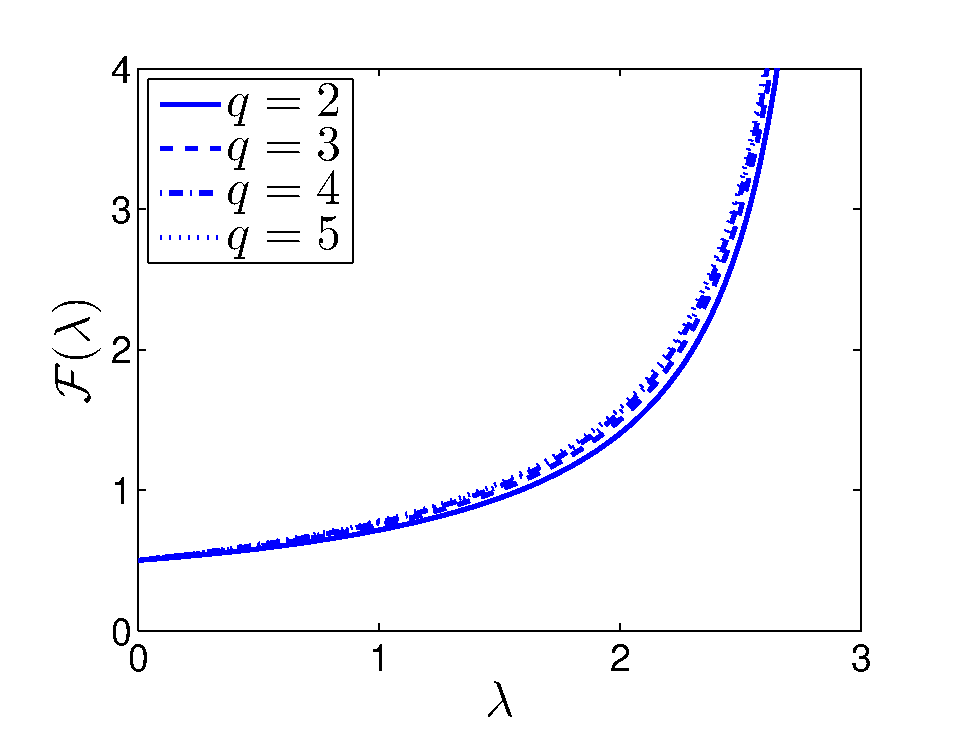
\includegraphics[width=9cm,height=4.8cm]{figs/ftreal}
\caption{\label{fig:conj_real}Plot of
  $\mathcal{F}(\lambda)$ on $0<\lambda<3$ for $q=2,3,4,5$. Note
  that $\mathcal{F}(0)={1/2}$ and that ${\mathcal F}(\lambda)\to +\infty$
  as $\lambda\to 3$ from below. We observe that $\mathcal{F}(\lambda)$ is 
  rather insensitive to changes in $q$.}
\end{figure}

In addition to the results (i), (ii), and (iv), which hold for all
$q>1$, we conjecture that the monotonicity result in (iii) holds not
just for $q=2,3,4$ but for all $q>1$. As additional support
of this conjecture, in Fig.~\ref{fig:conj_real} we plot the
numerically computed function ${\mathcal F}(\lambda)$ on $0<\lambda<3$
for $q=2,3,4,5$. 

\begin{conj}\label{conj:real} The monotonocity property (iii) of Proposition 
 \ref{rig:real_f} that ${\mathcal F}^{\prime}(\lambda)>0$ on
  $0<\lambda< 3$ holds for all $q>1$.
\end{conj}

Next, in order to count the number of eigenvalues of the NLEP 
(\ref{stab:nlep_final_1}) in $\mbox{Re}(\lambda)>0$ below, we need some
properties of $\mathcal{F}(\lambda)$, as defined in
(\ref{stab:merom_1}), as restricted to the non-negative imaginary axis.
By rewriting the operator as
\begin{equation*}
(L_{0}-i\lambda_{I})^{-1} = \left(L_{0}+i\lambda_{I}\right)
\left[\left(L_{0}+i\lambda_{I}\right)^{-1}(L_{0}-i\lambda_{I})^{-1}\right]
  = L_{0}\left[L_{0}^{2}+\lambda_{I}^{2}\right]^{-1}+
  i\lambda_{I}\left[L_{0}^{2}+\lambda_{I}^{2}\right]^{-1} \,,
\end{equation*}
we readily obtain upon upon separating 
${\mathcal F}(i\lambda_I)={\int w^{q-1}(L_{0}-i\lambda_{I})^{-1}w^{3}/
\int w^{q}}$ into real and imaginary parts that
\begin{equation}\label{eq:pol-F_R-F_I}
\mathcal{F}(i\lambda_{I})= {\mathcal F}_R(\lambda_I) + 
i {\mathcal F}_I(\lambda_I) \,; \qquad
\mathcal{F}_{R}(\lambda_{I})  =  \frac{\int w^{q-1}L_{0}
\left[L_{0}^{2}+\lambda_{I}^{2}\right]^{-1}w^{3}}{\int w^{q}} \,, \qquad
\mathcal{F}_{I}(\lambda_{I})  =  \frac{\lambda_{I}\int w^{q-1}
\left[L_{0}^{2}+\lambda_{I}^{2}\right]^{-1}w^{3}}{\int w^{q}} \,. 
\end{equation}
We then recall some rigorous results of \cite{mjww_1} for
$\mathcal{F}_{R}(\lambda_{I})$ and $\mathcal{F}_{I}(\lambda_{I})$ on
$\lambda_I\geq 0$.

\begin{proposition}\label{rig:imag_f} For $\lambda=i\lambda_I$ with
$\lambda_I> 0$, we have that
${\mathcal F}_R(\lambda_I)$ and ${\mathcal F}_I(\lambda_I)$ satisfy
\begin{itemize}
\item [{(i)}] $\mathcal{F}_{R}(\lambda_{I})={\mathcal O}(\lambda_{I}^{-2})
\quad \mbox{as}\quad \lambda_{I}\to+\infty\,,\quad\mathcal{F}_{R}(0)=1/2$.
\item [{(ii)}] $\mathcal{F}_{R}^{\prime}(\lambda_{I})<0\,, \quad \mbox{when}
\quad q=2,3 \,.$
\item [{(iii)}] $\mathcal{F}_{I}(\lambda_{I})=
{\mathcal O}(\lambda_{I}^{-1})\quad \mbox{as}\quad \lambda_{I}\to+\infty$.
\item [{(iv)}] $\mathcal{F}_{I}(\lambda_{I})\sim
\frac{\lambda_{I}}{4}\left(1-\frac{1}{q}\right)>0\quad \mbox{as}\quad
\lambda_{I}\to 0^{+}\,$.
\item [{(v)}] $\mathcal{F}_{I}(\lambda_{I})>0\,, \quad \mbox{when}\quad q=2,3,4$. 
\end{itemize}
\end{proposition}
\begin{proof} The statement in (i), and in (ii) for $q=2$, were proved
in Proposition 3.1 of \cite{mjww_1}; Statements (iii), (iv), and (v)
for $q=2,4$, were proved in Proposition 3.2 of \cite{mjww_1}. The
results in (ii) and (v) for $q=3$ follow by using the explicit formula
in (\ref{eq:exactF_q3}). For $q=3$, we have
$\mathcal{F}(i\lambda_{I}) = {3/\left[2({3-i\lambda_{I}})\right]}$, so
that
\begin{equation}
\mathcal{F}_{R}(\lambda_{I})=\frac{9}{2(9+\lambda_{I}^{2})}\,,\quad
\mathcal{F}_{R}^{\prime}(\lambda_{I})=-\frac{9\lambda_{I}}
        {\left(9+\lambda_{I}^{2}\right)^{2}}\,,\quad
        \mathcal{F}_{I}(\lambda_{I})=
        \frac{3\lambda_{I}}{2(9+\lambda_{I}^{2})}\,, \quad
\mathcal{F}_{I}^{\prime}(\lambda_{I})=
\frac{3(9-\lambda_I^2)}{2(9+\lambda_I^2)^2} \,, \quad
        \mbox{for} \quad q=3 \,.
\label{eq:pol-F_R-F_I-q=00003D3}
\end{equation}
This clearly shows that properties (ii) and (v) also hold for $q=3$.
\end{proof}

Although we only have a rigorous proof that
$\mathcal{F}_{R}^{\prime}(\lambda_{I})<0$ when $q=2,3$ and that
$\mathcal{F}_{I}(\lambda_{I})>0$ when $q=2,3,4$, we now conjecture
that these key properties hold for all $q>1$.  In
Fig.~\ref{fig:pol-F_R-F_I-for-q=00003D2to5} we plot the numerically
computed functions $\mathcal{F}_{R}(\lambda_{I})$ and
$\mathcal{F}_{I}(\lambda_{I})$ for various values of $q$, which give
numerical evidence for this conjecture. From this figure we observe that
 $\mathcal{F}_{R}(\lambda_{I})$ is rather insensitive to changes in $q$.

\begin{conj}\label{conj:imag}
\label{conj:pol-F(lambda)} Properties (ii) and (v) in Proposition
\ref{rig:imag_f} that $\mathcal{F}_{R}^{\prime}(\lambda_{I})<0$ and
$\mathcal{F}_{I}(\lambda_{I})>0$ on $\lambda_I>0$ hold for all
$q>1$.
\end{conj}

\begin{figure}[htbp]
\centering
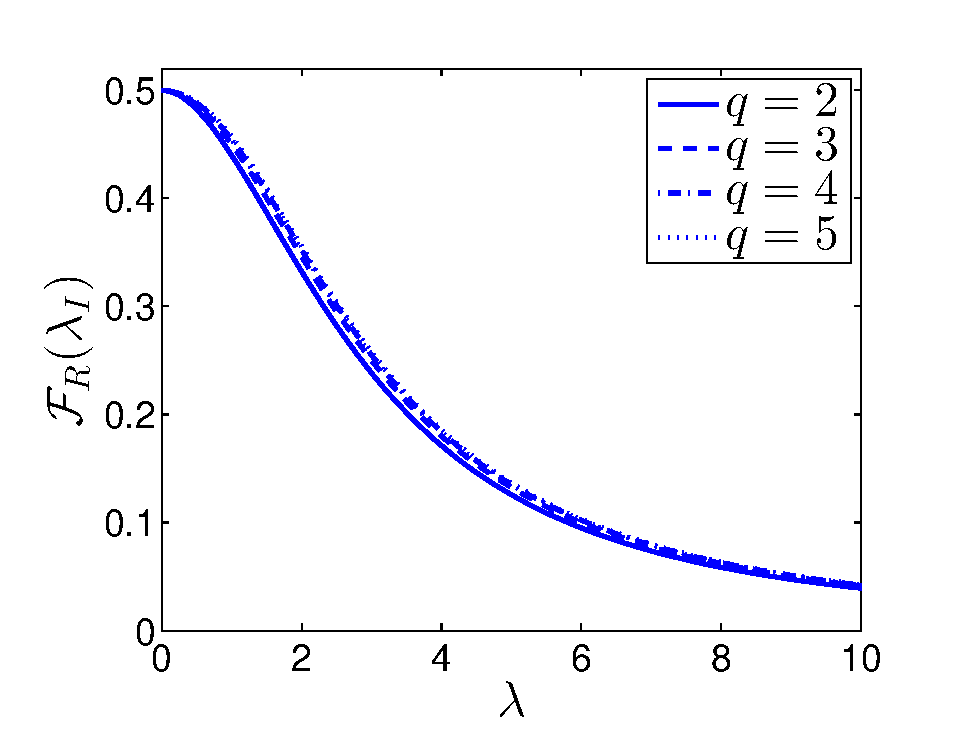
\includegraphics[width=9cm,height=4.8cm]{figs/freal}
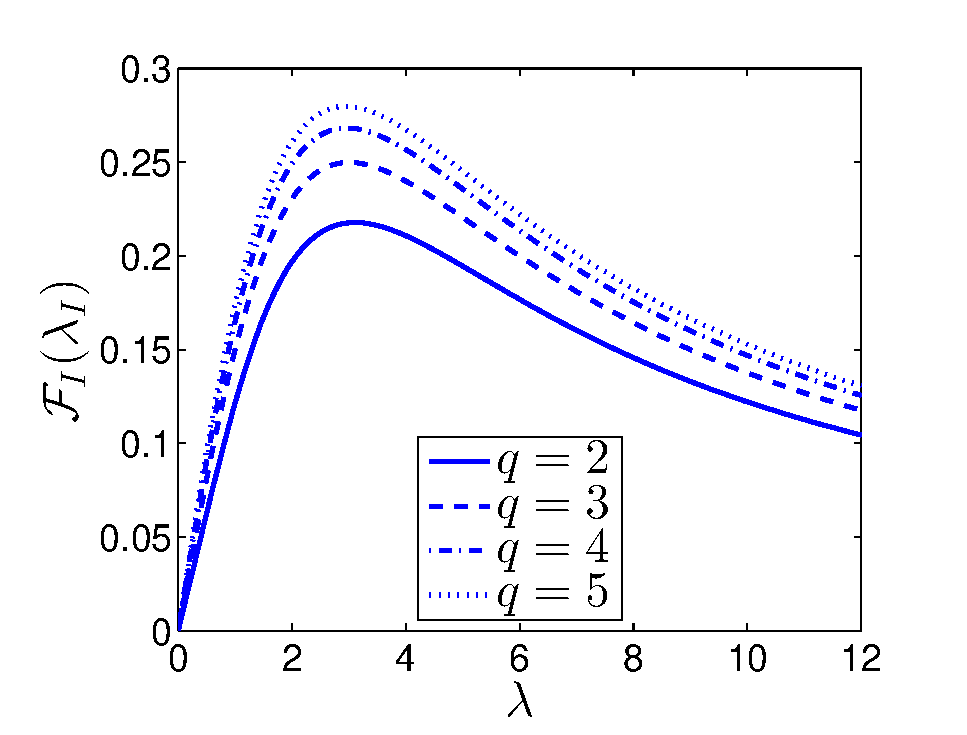
\includegraphics[width=9cm,height=4.8cm]{figs/fimag}
\caption{\label{fig:pol-F_R-F_I-for-q=00003D2to5}Plots of
  $\mathcal{F}_{R}(\lambda_I)$ (left panel) and
  $\mathcal{F}_{I}(\lambda_I)$ (right panel) for $q=2,3,4,5$. Note
  that $\mathcal{F}_{R}(0)=1/2$ and $\mathcal{F}_{I}(0)=0$, and that
  the maximum of $\mathcal{F}_{I}$ occurs near $\lambda_{I}=3$. In
  fact, the maximum does occur exactly at $\lambda_{I}=3$ when $q=3$.}
\end{figure}

\subsection{A Winding Number Criterion for the Number of Unstable Eigenvalues
of the NLEP}\label{sec:stab_arg}

We now use the argument principle of complex analysis to count the
number $N$ of eigenvalues of the NLEP (\ref{stab:nlep_final_1}) in
$\mbox{Re}(\lambda)>0$. For each $j=1,\ldots,K-1$, these discrete
eigenvalues are the complex zeroes of the function
$\zeta(\lambda)\equiv \mathcal{C}(\lambda)-\mathcal{F}(\lambda)$, as
defined in (\ref{stab:merom}). Here ${\mathcal F}(\lambda)$ is defined
in (\ref{stab:merom_1}) and from (\ref{stab:merom_2}) we have that
${\mathcal C}(\lambda)$ has the explicit form 
\bsub \label{stab:Cval}
\begin{equation}
\mathcal{C}(\lambda)=a(1+\tilde{\tau}_{j}\lambda)
\left(1-\frac{b}{3-\lambda}\right)\,, \label{stab:Cval_1}
\end{equation}
where $a$, $b$, and $\tilde{\tau}_{j}$, are defined for $j=1,\ldots,K-1$ by
\begin{equation} 
a\equiv \frac{\omega}{qU_{0}\chi_{0,j}} \,, \qquad
b\equiv \frac{9}{2} \chi_{0,j}\,, \qquad
\tilde{\tau}_{j} \equiv \frac{\hat{\tau}_{u}}{D_j \kappa_q} \,, \qquad
 \frac{1}{\chi_{0,j}} = 1 + \frac{\kappa_3 D_j}{\alpha} \,.
\label{stab:Cval_2}
\end{equation}
\esub
Here $\omega$ and $\kappa_q$ are given in (\ref{stab:kappa_omega}),
while $D_j$ and $\hat{\tau}_{u}$ are defined in (\ref{eq:pol-D_j}) and
\ref{eq:pol-tau-hat}, respectively.

From (\ref{stab:Cval_1}), $\mathcal{C}(\lambda)$ is a meromorphic
function with a simple pole at $\lambda=3$. Moreover,
$\mathcal{F}(\lambda)$ is analytic in $\mbox{Re}(\lambda)\geq 0$
except at the simple pole at $\lambda=3$. The simple poles of
$\mathcal{C}(\lambda)$ and $\mathcal{F}(\lambda)$ do not cancel as
$\lambda\to3^{-}$, since when restricted to the real line we get
$\mathcal{F}(\lambda)\to+\infty$ while
$\mathcal{C}(\lambda)\to-\infty$ as $\lambda\to 3^{-}$. Thus,
$\zeta(\lambda)=\mathcal{C}(\lambda)-\mathcal{F}(\lambda)$ has a
simple pole at $\lambda=3$.

\begin{figure}[htbp]
\centering
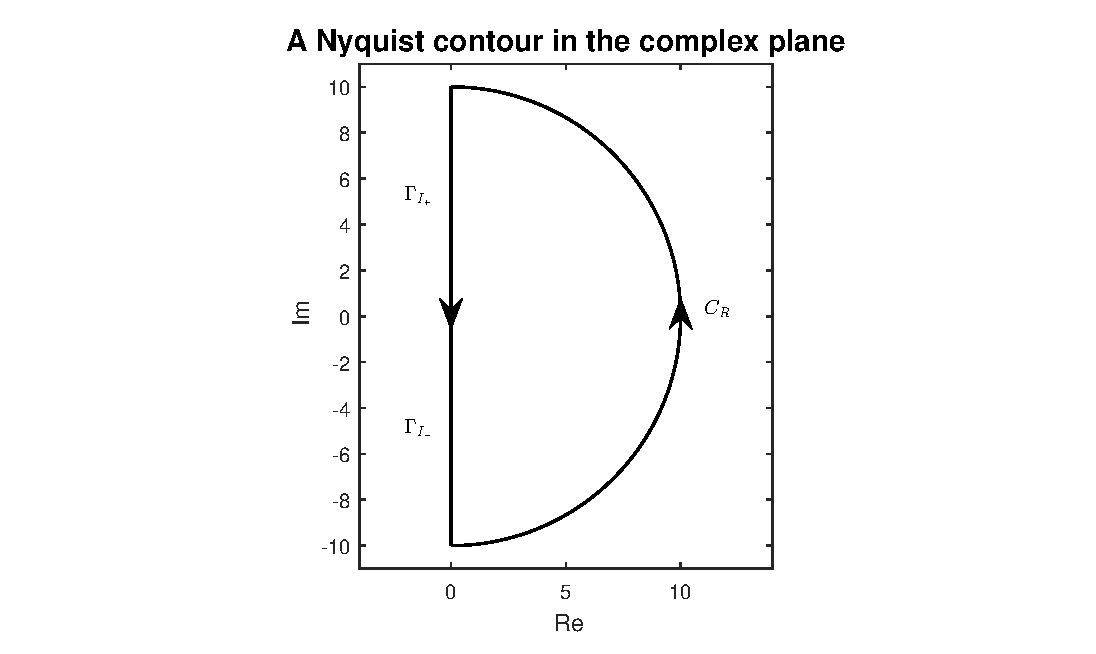
\includegraphics[width=13.0cm,height=4.8cm]{figs/nyq_cont}
\caption{\label{fig:nyquist}Schematic plot of the Nyquist contour
  $\Gamma$ used for determining the number $N$ of unstable eigenvalues
  of the NLEP (\ref{stab:nlep_final_1}).}
\end{figure}

To determine a formula for $N$, we calculate the winding of
$\zeta(\lambda)$ over the Nyquist contour $\Gamma$ traversed in the
counterclockwise direction that consists of the following segments in
the complex $\lambda$-plane (see the schematic in
Fig.~\ref{fig:nyquist}): $\Gamma_I^+$ ($0<\textrm{Im}(\lambda)<iR$,
$\textrm{Re}(\lambda)=0$), $\Gamma_I^-$ ($-iR<\textrm{Im}(\lambda)<0$,
$\textrm{Re}(\lambda)=0$), and $C_R$ defined by $|\lambda| = R >
0$ for $|\arg(\lambda)| < \pi/2$.

For each $j=1,\ldots,K-1$, $\zeta(\lambda)$ is analytic in
$\mbox{Re}(\lambda)\geq 0$ except at the simple pole $\lambda = 3$
corresponding to the unique positive eigenvalue of the local operator
$L_0$. Therefore, for each $j=1,\ldots,N-1$, and assuming that
$\zeta(\lambda)$ has no zeroes on the imaginary axis, we have by the
argument principle that $N = 1 + (2\pi)^{-1}\lim_{R\to\infty} \left[\arg
  \zeta \right]_\Gamma$, where $\left[\arg \zeta \right]_\Gamma$
denotes the change in the argument of $\zeta$ over $\Gamma$.  Since
${\mathcal F}(\lambda)={\mathcal O}(|\lambda|^{-1})$ on the
semi-circle $C_R$ as $R=|\lambda|\to \infty$, we have that
$\lim_{R\to\infty}\left[\arg \zeta \right]_{C_R}=
\lim_{R\to\infty}\left[\arg {\mathcal C} \right]_{C_R}$. From
(\ref{stab:Cval_1}) we calculate that $\lim_{R\to\infty}\left[\arg
  {\mathcal C} \right]_{C_R}=\pi$ when $\hat{\tau}_u>0$, and
$\lim_{R\to\infty}\left[\arg {\mathcal C} \right]_{C_R}=0$ when
$\hat{\tau}_u=0$.  For the contour $\Gamma_I^-$, we use that
$\zeta(\overline{\lambda}) = \overline{\zeta(\lambda)}$ so that
$\left[\arg \zeta \right]_{\Gamma_I^-} = \left[\arg
  \zeta\right]_{\Gamma_I^+}$.  In this way, for each $j=1,\ldots,K-1$,
we conclude that
\begin{equation}
  N = \frac{3}{2} + \frac{1}{\pi} \left[\arg \zeta \right]_{\Gamma_I^{+}} \,,
 \quad \mbox{for} \quad \hat{\tau}_u>0 \,; \qquad
  N = 1 + \frac{1}{\pi} \left[\arg \zeta \right]_{\Gamma_I^{+}} \,,
 \quad \mbox{for} \quad \hat{\tau}_u=0 \,. \label{key:wind}
\end{equation}
Here $\left[\arg \zeta \right]_{\Gamma_I^{+}}$ denotes the change
in the argument of $\zeta$ as the imaginary axis $\lambda=i\lambda_I$ is
traversed from $\lambda_I=+\infty$ to $\lambda_I=0$.

We remark that (\ref{key:wind}) determines the number of unstable
eigenvalues of the NLEP (\ref{stab:nlep_final_1}) for any {\em
  specific} asynchronous mode $j=1,\ldots,K-1$. The total number of
such unstable eigenvalues, for all asynchronous modes, is simply the
union of (\ref{key:wind}) over $j=1,\ldots,K-1$. In this way, the
problem of determining $N$ for a particular mode $j$ is reduced to
calculating the change of argument of $\zeta(\lambda)= {\mathcal
  C}(\lambda)-{\mathcal F}(\lambda)$ as we traverse down the positive
imaginary axis. To do so, we will need the properties of ${\mathcal
  F}(i\lambda_I)$ given in Proposition \ref{rig:imag_f}, together with
results for ${\mathcal C}(i\lambda)$ to be obtained from
(\ref{stab:Cval}).

\subsection{The Competition Instability Threshold}\label{sec:stab_compt}

We now determine the competition instability threshold value of the
diffusivity ${\mathcal D}_0$, which is characterized by a zero-eigenvalue 
crossing of the NLEP (\ref{stab:nlep_final_1}). Since
${\mathcal F}(0)={1/2}$ (see (i) of Proposition \ref{rig:real_f}), we
conclude that $\zeta(0)=0$ when ${\mathcal C}(0)={1/2}$. From using
(\ref{stab:merom_2}), or equivalently (\ref{stab:Cval}), for
${\mathcal C}(\lambda)$ we conclude that $\lambda=0$ when
\begin{equation}\label{stab:zero_1}
   \frac{\omega}{qU_0} \left( \frac{1}{\chi_{0,j}} - \frac{3}{2}\right)=
\frac{1}{2} \,, \qquad j=1,\ldots,K-1\,.
\end{equation}
By using (\ref{stab:Cval_2}) for $\chi_{0,j}$, together with
(\ref{stab:kappa_omega}) for $\kappa_3$, (\ref{stab:zero_1}) yields
that $\lambda=0$ when
\begin{equation}\label{stab:zero_2}
   D_j = \frac{\omega^3}{4\pi^2 K^3 \alpha^2} 
\left( 1+ \frac{qU_0}{\omega} \right) \,, \qquad j=1,\ldots,K-1 \,.
\end{equation}
Finally, by using $D_j=2 K {\mathcal D}_0{\left(1-\cos({\pi j/K})\right)/S}$, as
obtained from (\ref{eq:pol-D_j}), we conclude that the NLEP has a 
zero-eigenvalue crossing at the $K-1$ distinct values ${\mathcal D}_{0,j}$
of ${\mathcal D}_0$ given by
\begin{equation}\label{stab:zero_final}
    {\mathcal D}_{0,j} = \frac{\omega^3 S}{8 \pi^2 \alpha^2 K^4 
  \left(1 - \cos\left({\pi j/K}\right)\right)} \left( 1 + \frac{q U_0}{\omega}
  \right) \,, \qquad j=1,\ldots,K-1\,.
\end{equation}
As we show in Proposition \ref{prop:comp_t} below, the competition
instability threshold ${\mathcal D}_{0,c}$ corresponds to the
smallest such ${\mathcal D}_{0,j}$, which occurs when $j=K-1$. This yields that
\begin{equation}\label{stab:zero_d0min}
   {\mathcal D}_{0,c}\equiv {\mathcal D}_{0,K-1} = \frac{\omega^3 S}{8
     \pi^2 \alpha^2 K^4 \left(1 + \cos\left({\pi /K}\right)\right)}
   \left( 1 + \frac{q U_0}{\omega} \right) \,.
\end{equation}
In terms of the unscaled diffusivity $D=\epsilon^{-2}{\mathcal D}_0$,
the competition stability threshold occurs at
$D_{c}\equiv \epsilon^{-2}{\mathcal D}_{0,c}$.

\begin{rem}\label{stab:zero_two_nonlocal} The zero-eigenvalue crossing
condition (\ref{stab:zero_1}) can also be obtained from the NLEP
(\ref{stab:nlep_old}) with two nonlocal terms by setting $\Phi=w$ and
$\lambda=0$ in (\ref{stab:nlep_old}). By using the identity $L_0 w= 2
w^3$, this substitution yields $2-3\chi_{0,j} - q \chi_{1,j}=0$, where
from (\ref{stab:newchi}) we have $\chi_{1,j}={U_0 \chi_{0,j}/\omega}$
at $\lambda=0$. Some simple algebra then recovers (\ref{stab:zero_1}).
\end{rem}

\noindent We now prove an instability result related to
zero-eigenvalue crossings:

\begin{prop}
\label{prop:comp_t} For $\epsilon\to 0$, $K\geq 2$, $q>1$, 
$0<U_0<U_{0,\max}$, ${\mathcal D}_0=\epsilon^2 D = {\mathcal
  O}(1)$, a $K$-hotspot steady-state solution for (\ref{eq:pol-main})
is unstable for all $\hat{\tau}_u\geq 0$ when ${\mathcal
  D}_0>{\mathcal D}_{0,c}$, where ${\mathcal D}_{0,c}$ is the
competition stability threshold defined in
(\ref{stab:zero_d0min}). For ${\mathcal D}_0<{\mathcal D}_{0,c}$, a
$K$-hotspot steady-state is linearly stable when $\hat{\tau}_u=0$ and
$q=2,3,4$.
\end{prop}

\begin{proof} We first prove that when ${\mathcal D}_0>{\mathcal D}_{0,c}$,
then $\zeta(\lambda)=0$ in (\ref{stab:merom}) has a positive real root
in $0<\lambda<3$ for each $j=1,\ldots,K-1$. This readily follows from
the fact that ${\mathcal C}(0)>{1/2}$ for each $j=1,\ldots,K-1$, that
${\mathcal C}(\lambda)\to -\infty$ as $\lambda\to 3^{-}$, and
from Proposition \ref{rig:real_f} where we have ${\mathcal
  F}(0)={1/2}$ and ${\mathcal F}(\lambda)\to +\infty$ as $\lambda\to
3^{-}$. Thus, by continuity, there is at least one positive real root
to $\zeta(\lambda)=0$ on $0<\lambda<3$ for each $j=1,\ldots,K-1$ and
for any $\hat{\tau}_u\geq 0$. Next, for ${\mathcal D}_0<{\mathcal
  D}_{0,c}$, we show that $N=0$ by using the winding number
criterion (\ref{key:wind}) and calculating $\left[\arg \zeta
  \right]_{\Gamma_I^{+}}$ explicitly.  From (\ref{stab:Cval_1}), we
decompose ${\mathcal C}(i\lambda_I)={\mathcal C}_R(\lambda_I) +
i{\mathcal C}_I(\lambda_I)$, and for $\hat{\tau}_u=0$ calculate that
\begin{equation*}
   {\mathcal C}_I(\lambda_I) = -\frac{ a b \lambda_I}{9+\lambda_I^2} < 0
\qquad \mbox{for} \quad \lambda_I>0 \,.
\end{equation*}
Since ${\mathcal F}_I(\lambda_I)>0$ for $\lambda_I>0$ for $q=2,3,4$ from
property (v) of Proposition \ref{rig:imag_f}, we conclude that
$\mbox{Im}\left[\zeta(i\lambda_I)\right]<0$ for $\lambda_I>0$. Then, since
${\mathcal C}(0)>{1/2}$ when ${\mathcal D}_0<{\mathcal D}_{0,c}$,
and ${\mathcal F}(0)={1/2}$ from (i) of Proposition \ref{rig:real_f}, 
we have $\zeta(0)>0$ for each $j=1,\ldots,K-1$, and $\zeta(i\lambda_I)
\to {\omega/(qU_0\chi_{0,j})}>0$ as $\lambda_I\to +\infty$. It follows that
$\left[\arg \zeta \right]_{\Gamma_I^{+}}=-\pi$, and consequently $N=0$ from
the second statement in (\ref{key:wind}) for $\hat{\tau}_u=0$.
\end{proof}

We remark that if Conjecture \ref{conj:imag} holds, then a $K$-hotspot
steady-state is linearly stable when ${\mathcal D}_0<{\mathcal
  D}_{0,c}$ and $\hat{\tau}_u=0$ for any $q>1$. Moreover, by
continuity of eigenvalue paths in $\hat{\tau}_u$, the stability result
in Proposition \ref{prop:comp_t} should hold for all $\hat{\tau}_u>0$
but sufficiently small. The possibility of Hopf bifurcations values of
$\hat{\tau}_u$ for the range ${\mathcal D}_0<{\mathcal D}_{0,c}$ is
examined for $q=3$ in \S \ref{sec:stab_q3} and for general $q>1$ in
\S \ref{sec:stab_qn3}.

\subsection{Qualitative Interpretation of the Competition Instability Threshold}\label{sec:qual_comp_d}

Next, we discuss the qualitative behavior of the competition
instability threshold ${\mathcal D}_{0,c}$ with respect to the degree
$q$ of patrol focus and the total level $U_0$ of police patrol
deployment.  From (\ref{eq:amax}), the maximum $A_{\max}$ of the
steady-state attractiveness field is $A_{\max}\sim
\epsilon^{-1}{\omega/(K\pi)}$, which decreases as either $\omega$
decreases or $K$ increases. However, from Corollary
\ref{cor:pol-K-hotspots-in-A-rho-U}, the amplitude of the steady-state
criminal density $\rho$ at the hotspot locations is
$\rho_{\max}=\left[w(0)\right]^2=2$, which is independent of all model
parameters, while away from the maxima of $A$ the criminal density is
${\mathcal O}(\epsilon^{2})\ll 1$. Therefore, it is the reduction of
the number of stable steady-state hotspots on a given domain length
that is the primary factor in reducing the total crime in the
domain. As such, we seek to tune the police parameters $q$ and $U_{0}$
so that the range of diffusivity ${\mathcal D}_{0}$ for which a
$K$-hotspot steady-state is unconditionally unstable, i.e.~unstable
for all $\hat{\tau}_u>0$, is as large as possible. This corresponds to
minimizing the competition stability threshold ${\mathcal D}_{0,c}$ in
(\ref{stab:zero_d0min}).

From (\ref{stab:zero_d0min}), we observe that ${\mathcal D}_{0,c}$
increases with $q$ in a linear fashion. Within the context of our RD
model (\ref{eq:pol-main}), this predicts that if the police become
increasingly focused on patrolling the more crime-attractive areas,
then paradoxically the range of ${\mathcal D}_{0}$ where a $K$-hotspot
steady-state is unstable decreases. Therefore, for the goal of
reducing the number of stable crime hotspots, a police deployment with
intense focus on crime-attractive areas does not offer an advantage
over that of a less focused patrol (assuming that $q>1$ for our
analysis to hold). At a fixed level $U_0$ of police deployment, and for
integer values of $q$ with $q>1$, the best patrol strategy
is to take $q=2$, which corresponds to the ``cops-on-the-dots''
strategy (cf.~\cite{jbc}, \cite{rick}, \cite{zipkin}) where the police
mimic the movement of the criminals.

For a fixed $q>1$, we next examine how the competition stability
threshold for a $K$-hotspot steady-state changes with the total police
deployment $U_{0}$.  To this end, we substitute
$U_{0}=S(\gamma-\alpha) - \omega$ into (\ref{stab:zero_d0min}),
and write ${\mathcal D}_{0,c}$ as
\begin{equation}
   {\mathcal D}_{0,c} = \frac{S}{8 \pi^2 \alpha^2 K^4 \left(1
      + \cos\left({\pi /K}\right)\right)} \, g(U_0) \,, \qquad
 g(U_0) \equiv\omega^{3}(1-q)+qS(\gamma-\alpha)\omega^{2}\,; \qquad
   \omega \equiv S(\gamma-\alpha) - U_0 \,. \label{eq:pol-D0*-g(w)}
\end{equation}
To analyze the critical points of $g(U_0)$, we first observe that 
${d\omega/dU_{0}}=-1$ and that $U_{0}\to U_{0,\max}=S(\gamma-\alpha)$ as 
$\omega \to 0$. We then calculate that
\begin{equation*}
\frac{dg}{dU_{0}}  =  -3 (1-q) \omega \left(\omega-\omega_c\right) \,,
\qquad \mbox{where}\qquad \omega_{c}\equiv 
\frac{2qS(\gamma-\alpha)}{3(q-1)}\,.
\end{equation*}
We conclude that $\omega_c<S(\gamma-\alpha)$, so that
$0<U_0<U_{0,\max}$, iff $q>3$. Therefore, $g(U_0)$ has a unique maximum
point on $0<U_0<U_{0,\max}$ iff $q>3$.  Alternatively, for $q\leq 3$
we have ${dg/dU_{0}}<0$ for $0<U_{0}<U_{0,\max}$.

Therefore, ${\mathcal D}_{0,c}$ is monotonically decreasing in $U_{0}$
when the patrol focus satisfies $q\leq 3$. For $q\leq 3$, increasing
the level $U_0$ of police deployment leads to a larger range of
${\mathcal D}_0$ where the $K$-hotspot steady-state is unconditionally
unstable.  However, if $q>3$, then initially as $U_0$ is increased
from zero, the range of ${\mathcal D}_0$ where the steady-state
hotspot pattern is unstable is decreased, until the critical value
$U_{0,c} \equiv
S(\gamma-\alpha)-\omega_{c}=S(\gamma-\alpha){(q-3)/[3(q-1)]}$ is
reached. For $U_0>U_{0,c}$, the hotspot pattern becomes less stable
when the policing level is increased. These qualitative results are
displayed in Fig.~\ref{fig:gU0-vs-U0}.

Finally, we can interpret our competition stability threshold in terms
of a critical threshold $K_{c}$ for which a steady-state pattern of
$K\geq 2$ hotspots is unconditionally unstable when $K>K_{c}$.  This
instability, which develops on an ${\mathcal O}(1)$ time scale as
$\eps\to 0$, is due to a real positive eigenvalue of the NLEP, and as
we show from full numerical simulations in \S \ref{sec:numerics_q3}
and in \S \ref{sec:numerics_qn3} it triggers the collapse of some of
the hotspots in the pattern. By writing (\ref{eq:pol-D0*-g(w)}) in
terms of $K$, this critical threshold $K_{c}>0$ when $D={{\mathcal
    D}_0/\epsilon^2}$, and where $g(U_0)$ is defined in
(\ref{eq:pol-D0*-g(w)}), is the unique root of
\begin{equation}
  K \left[ 1 + \cos\left({\pi/K}\right)\right]^{1/4} =
 \frac{\left({S/D}\right)^{1/4}}{2^{3/4} \sqrt{\pi \epsilon \alpha}} \left[
   g(U_0) \right]^{1/4} \,. \label{stab:Kc+}
\end{equation}


\begin{figure}[htbp]
\centering
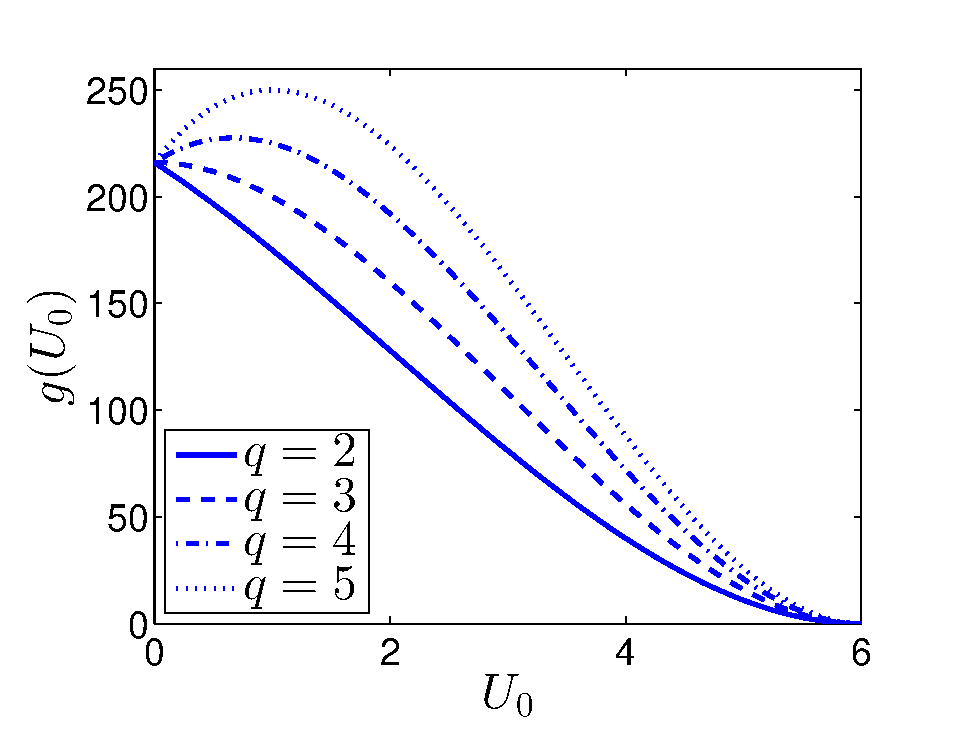
\includegraphics[width=9cm,height=4.8cm]{figs/comp_gplot}
\caption{\label{fig:gU0-vs-U0}Competition instability threshold
  nonlinearity $g(U_{0})$, as defined in (\ref{eq:pol-D0*-g(w)}), versus
  total police deployment $U_{0}$ for patrol focus parameters
  $q=2,3,4,5$. Other model parameters are $S=6$, $\gamma=2$, $\alpha=1$, so
  that $U_{0,\max}=6$ as shown in the right-most tick of the figure.
  The competition instability threshold ${\mathcal D}_{0,c}$ is
  simply a positive scaling of $g(U_{0})$ according to
  (\ref{eq:pol-D0*-g(w)}).}
\end{figure}

\setcounter{equation}{0}
\setcounter{section}{4}
\section{Explicitly Solvable Case $q=3$: Asynchronous Hotspot Oscillations}
\label{sec:stab_q3}

For each $j=1,\ldots,K-1$, we now analyze the quadratic equation
(\ref{stab:q3_quad}) in the eigenvalue parameter $\lambda$
characterizing the discrete spectrum of the NLEP
(\ref{stab:nlep_final_1}) for the special case where $q=3$. In terms
of the coefficients of the quadratic (\ref{stab:q3_quad_1}), for each
$j=1,\ldots,K$ the eigenvalues $\lambda_1$ and $\lambda_2$ satisfy
\begin{equation}\label{q3:lam12}
   \lambda_1 \lambda_2 = \frac{c_0}{c_2} \,, \qquad
  \lambda_1 + \lambda_2 = - \frac{c_1}{c_2} \,,
\end{equation}
where $c_0$, $c_1$, and $c_2>0$, are given in (\ref{stab:q3_quad_2}). For
the $j$-th mode, we conclude that $\mbox{Re}(\lambda)<0$ when $c_0>0$
and $c_1>0$. We have instability of the $j$-th mode if either
$c_0<0$, or if $c_0>0$ and $c_1<0$. We have purely complex eigenvalues,
corresponding to a Hopf bifurcation point, when $c_0>0$ and $c_1=0$.

We first determine the signs of $c_0$ and $c_1$ in terms of $D_j$ and
$\hat{\tau}_{u}$. From (\ref{stab:q3_quad_2}) we observe that $c_0=0$
when the zero-eigenvalue crossing condition (\ref{stab:zero_1}) holds,
which yields (\ref{stab:zero_2}) for $D_j$, which we relabel as
\begin{equation}\label{q3:dup}
     D_j = \dustar \equiv \frac{\omega^3}{4\pi^2 K^3 \alpha^2}
  \left( 1 + \frac{3U_0}{\omega}\right) \,.
\end{equation}
Next, we set $c_1=0$ in (\ref{stab:q3_quad_2}) to get, using
(\ref{stab:newchi}) for $\chi_{0,j}^{-1}$, that
\begin{equation}\label{q3:c1zero_old}
  \frac{\hat{\tau}_u}{D_j \kappa_3} = \frac{2 \chi_{0,j}^{-1}}
  {3 \left( 2 \chi_{0,j}^{-1} -3 \right)} = \frac{1}{3}
  \frac{ \left(D_j + {\alpha/\kappa_3}\right)}{\left(D_{j}- 
  {\alpha/(2\kappa_3)}\right)} \,.
\end{equation}
The denominator of this expression motivates introducing $\dlstar$,
defined by
\begin{equation}\label{q3:dlow}
    \dlstar \equiv \frac{\alpha}{2\kappa_3} =
 \frac{\omega^3}{4\pi^2 K^3 \alpha^2} \,,
\end{equation}
where we have used the expression (\ref{stab:kappa_omega}) for
$\kappa_3$. Upon using (\ref{q3:dlow}) in (\ref{q3:c1zero_old}), we
obtain that $c_1=0$ when $\hat{\tau}_u$ satisfies
\bsub \label{q3:c1zero}
\begin{equation}
   \hat{\tau}_u = \hat{\tau}_{uH,j}\equiv {\mathcal H}\left({D_j/\dlstar}\right)
  \,, \qquad j=1,\ldots,K-1 \,,
\end{equation}
where the function ${\mathcal H}(\beta)$ is defined by
\begin{equation}\label{q3:h}
   {\mathcal H}(\beta) \equiv \frac{\alpha \beta}{2} \left(
  \frac{1}{3} + \frac{1}{\beta -1} \right) \,.
\end{equation}
\esub
Notice that $\hat{\tau}_{uH,j}>0$ only when $D_j>\dlstar$.  Some simple
algebra then shows that we can write $c_1$ in (\ref{stab:q3_quad_2}) as
\begin{equation}\label{q3:c1_new}
  c_1 = \frac{1}{\alpha} \left( \frac{\dlstar}{D_j}-1\right)
  \left(\hat{\tau}_u - \hat{\tau}_{uH,j}\right) \,.
\end{equation}
For the $j$-th mode, we have $c_1<0$ if $D_j>\dlstar$ and
$\hat{\tau}_u>\hat{\tau}_{uH,j}$, while $c_1>0$ if either
$D_j<\dlstar$, or $D_j>\dlstar$ and $\hat{\tau}_u<\hat{\tau}_{uH,j}$.
With these signs for $c_0$ and $c_1$, we summarize our stability
result for the $j$-th mode so far as follows:
\begin{itemize}
  \item For $D_j>\dustar$ ($c_0<0$), we have $\mbox{Re}(\lambda)>0$, and
        instability is due to a positive real eigenvalue.
  \item For $D_j<\dlstar$ ($c_0>0$ and $c_1>0$), we have stability
        $\mbox{Re}(\lambda)<0$.
  \item On the range $\dlstar<D_j<\dustar$ $(c_0>0)$, we have
    instability if $\hat{\tau}_u>\hat{\tau}_{uH,j}$ $(c_1<0)$ and
    stability if $\hat{\tau}_u<\hat{\tau}_{uH,j}$ $(c_1>0)$. On this
    range of $D_j$, the Hopf bifurcation threshold,
    $\hat{\tau}_{uH,j}>0$, is given in (\ref{q3:c1zero}). 
\end{itemize}

Next, we must reformulate this result in terms of ${\mathcal D}_0$
rather than $D_j$, by using $D_j={\mathcal D}_0 \left({2K/S}\right)
\left(1-\cos\left({\pi j/K}\right)\right)$. The interval 
$\dlstar<D_1<\dustar$, where a Hopf bifurcation value of $\hat{\tau}_u$ 
exists, becomes
\begin{equation}\label{q3:interval_old}
 \frac{S\dlstar}{2K\left(1-\cos\left(\pi j/K\right)\right)} \leq {\mathcal D}_0
 \leq \frac{S\dustar}{2K\left(1-\cos\left(\pi j/K\right)\right)} \,,
\end{equation}
where ${\dustar/\dlstar}=1+{3U_0/\omega}$ from (\ref{q3:dup}) and
(\ref{q3:dlow}). It is convenient to write (\ref{q3:interval_old}) in
terms of the competition stability threshold ${\mathcal D}_{0,c}$
defined by setting $q=3$ in (\ref{stab:zero_d0min}). In this way, the
interval in (\ref{q3:interval_old}) becomes 
\bsub \label{q3:interval}
\begin{equation}
   \dzjm < {\mathcal D}_0 <\dzjp \,; \qquad
   \dzjp \equiv {\mathcal D}_{0,c} \left( \frac{1+\cos\left({\pi/K}\right)}
  {1-\cos\left({\pi j /K}\right)}\right) \,, \qquad
   \dzjm \equiv \frac{{\mathcal D}_{0,c}}{\left(1+{3U_0/\omega}\right)}
  \left( \frac{1+\cos\left({\pi/K}\right)}
  {1-\cos\left({\pi j /K}\right)}\right) \,, \label{q3:interval_1}
\end{equation}
where ${\mathcal D}_{0,c}$ is given by
\begin{equation}
{\mathcal D}_{0,c}\equiv \frac{\omega^3 S}{8
     \pi^2 \alpha^2 K^4 \left(1 + \cos\left({\pi /K}\right)\right)}
   \left( 1 + \frac{3 U_0}{\omega} \right) \,. \label{q3:interval_2}
\end{equation}
\esub
We observe that when $j=K-1$, we have $D^{+}_{0,K-1}={\mathcal D}_{0,c}$.
Now since ${D_j/\dlstar}={{\mathcal D}_0/\dzjm}$, the Hopf bifurcation
threshold in (\ref{q3:c1zero}) becomes
\begin{equation}\label{q3:hopf}
   \hat{\tau}_{uH,j} = {\mathcal H}\left({{\mathcal D}_0/\dzjm}\right)
   \,, \qquad \mbox{on} \quad  \dzjm < {\mathcal D}_0 <\dzjp \,.
\end{equation}
From this expression, we readily derive the following limiting
behavior for $\hat{\tau}_{uH,j}$ at the two ends of the interval:
\begin{equation}\label{q3:tau_lim}
 \hat{\tau}_{uH,j} \sim \frac{\alpha}{2} \left[ \frac{{\mathcal D}_0}
 {D^{-}_{0,j}}-1 \right]^{-1} \,, \quad \mbox{as} \quad
{\mathcal D}_0\to \dzjm\,; \qquad
 \hat{\tau}_{uH_j}\sim \frac{\omega \alpha}{6 U_0} \left( \frac{U_0}{\omega}
  + 1 \right) \left( \frac{3U_0}{\omega} + 1\right) \,, \quad \mbox{as}
  \quad {\mathcal D}_0\to \dzjp \,.
\end{equation}

For each fixed $j=1,\ldots,K-1$, we summarize the behavior of the roots
of the quadratic (\ref{stab:q3_quad}), corresponding to the discrete
eigenvalues of the NLEP (\ref{stab:nlep_final_1}) as follows:

\begin{prop}\label{q3:roots_quad} For each fixed $j=1,\ldots,K-1$,
let $\lambda_{+}$ and $\lambda_{-}$, with
$\mbox{Re}(\lambda_{+})\geq\mbox{Re}(\lambda_{-})$, denote the two
solutions of the quadratic equation (\ref{stab:q3_quad}). Then, their
location in the complex plane depends on ${\mathcal D}_0$ and
$\hat{\tau}_u$ as follows:
\begin{itemize}
  \item For ${\mathcal D}_0>\dzjp$, we have $\lambda_+>0$ and $\lambda_-<0$
     for all $\hat{\tau}_u\geq 0 \,.$
  \item For ${\mathcal D}_0<\dzjm$, we have $\mbox{Re}(\lambda_{\pm})<0$
     for all $\hat{\tau}_u\geq 0 \,.$
  \item For $\dzjm<{\mathcal D}_0<\dzjp$ we have $\mbox{Re}(\lambda_{\pm})>0$
   when $\hat{\tau}_u>\hat{\tau}_{uH,j}$ and $\mbox{Re}(\lambda_{\pm})<0$ when
   $0\leq \hat{\tau}_{uH,j}<\hat{\tau}_u$.
\end{itemize}
Here $\dzjm$ and $\dzjp$ are defined in (\ref{q3:interval_1}). The
Hopf bifurcation threshold $\hat{\tau}_{uH,j}$, which is defined on
the interval $\dzjm < {\mathcal D}_0 <\dzjp$, is given in
(\ref{q3:hopf}).
\end{prop}

Since ${\dzjp/\dzjm}=1+{3U_0/\omega}$, we observe that the width of
the interval $\dzjm<{\mathcal D}_0<\dzjp$ where an asynchronous
oscillatory instability in the hotspot amplitudes occurs is nonzero only as
a result of the simple coupling term $-U$ in our three-component RD
system (\ref{eq:crs-main}). In the absence of police, this interval
disappears and the basic crime model does not support oscillatory
instabilities in this parameter regime.

Next, we examine the monotonicity properties of the universal function 
${\mathcal H}(\beta)$ characterizing Hopf bifurcations, as defined
in (\ref{q3:h}), on the interval $1<\beta<{\dzjp/\dzjm}=1+{3U_0/\omega}$.
We calculate ${\mathcal H}^{\prime}(\beta)$ to get
\begin{equation*}
   {\mathcal H}^{\prime}(\beta) = \frac{\alpha}{6 (\beta-1)^2} \left[
  (\beta-1)^2 -3 \right] \,,
\end{equation*}
so that ${\mathcal H}^{\prime}(\beta)<0$ if $1<\beta<1+\sqrt{3}$ and
${\mathcal H}^{\prime}(\beta)>0$ if $\beta>1+\sqrt{3}$. We conclude
that ${\mathcal H}^{\prime}(\beta)<0$ on $1<\beta<1+{3U_0/\omega}$ only
when $\omega>\sqrt{3}U_0$. Since $\omega=S(\gamma-\alpha)-U_0$ we conclude
that
\begin{equation}\label{q3:hmonot}
   {\mathcal H}^{\prime}(\beta)<0 \, \quad \mbox{on} \quad 1<\beta<{3U_0/\omega}
  \,, \quad \mbox{iff} \quad U_0 < \frac{S(\gamma-\alpha)}{1+\sqrt{3}} \,.
\end{equation}
If $\frac{S(\gamma-\alpha)}{1+\sqrt{3}}<U_0<U_{0,\max}$, then
${\mathcal H}(\beta)$ increases on $1+\sqrt{3}<\beta<1+{3U_0/\omega}$.

Next, we rewrite the coefficients $c_0$, $c_1$, and $c_2$, in the
quadratic (\ref{stab:q3_quad}) so as to readily calculate the Hopf
bifurcation eigenvalue $\lambda=i\lambda_{IH}$. After some algebra we
obtain that
\begin{equation}\label{q3:new_c0c1c2}
  c_0 = -\frac{1}{2}\left(1+\frac{3U_0}{\omega}\right)
   \left( \frac{{\mathcal D}_0}{\dzjp}-1\right) \,, \qquad
  c_1 = \frac{\hat{\tau}_{uH,j}}{\alpha} \left( \frac{\dzjm}{{\mathcal D}_0}
  -1 \right)\left( \frac{\hat{\tau}_u}{\hat{\tau}_{uH,j}} -1 \right) \,,
  \qquad c_2 = \frac{\hat{\tau}_{uH,j}}{3\alpha}
  \left(\frac{2\dzjm}{{\mathcal D}_0} + 1 \right) \,,
\end{equation}
where $\hat{\tau}_{uH,j}$ is defined in (\ref{q3:hopf}). The Hopf bifurcation
eigenvalue $\lambda=i\lambda_{IH}$ with $\lambda_{IH}>0$ is 
$\lambda_{IH}=\sqrt{c_0/c_2}$, which yields
\begin{equation}\label{q3:dlami}
   \lambda_{IH}=\frac{3}{\left(2 + {{\mathcal D}_0/\dzjm}\right)} 
  \sqrt{ \left( 1 + \frac{3U_0}{\omega}\right) 
    \left(1 - \frac{{\mathcal D}_0}{\dzjp}\right)
\left(\frac{{\mathcal D}_0}{\dzjm} -1 \right)}\,, \quad \mbox{on} \quad
   \dzjm < {\mathcal D}_0 < \dzjp \,.
\end{equation}
This shows that $\lambda_{IH}$ vanishes at both endpoints.  We use the
asymptotic behaviors ${{\mathcal D}_0/\dzjp}\to
\left(1+{3U_0/\omega}\right)^{-1}$ as ${\mathcal D}_0\to \dzjm$ and
${{\mathcal D}_0/\dzjm}\to \left(1+{3U_0/\omega}\right)$ as ${\mathcal
  D}_0\to \dzjp$, so that from (\ref{q3:dlami}) we obtain the limiting
asymptotic behavior
\begin{equation}\label{q3:lim_val}
   \lambda_{IH}\sim \frac{1}{\left(1 + {U_0/\omega}\right)}
  \sqrt{ \frac{3U_0}{\omega} \left( 1 + \frac{3U_0}{\omega}\right) 
    \left(1 - \frac{{\mathcal D}_0}{\dzjp}\right)} \quad \mbox{as}
 \quad {\mathcal D}_0\to \dzjp\,; \qquad
  \lambda_{IH}\sim \sqrt{ \frac{3U_0}{\omega} 
  \left( \frac{{\mathcal D}_0}{\dzjm}-1\right)} \quad \mbox{as} \quad
  {\mathcal D}_0\to \dzjm \,.
\end{equation}

\noindent For the special case $K=2$, we now state our main result stability
result related to Hopf bifurcations.

\begin{prop}\label{q3:main_twospots} For $\epsilon\to 0$, 
$q=3$, $0<U_0<U_{0,\max}$, $\hat{\tau}_u\ll {\mathcal
    O}(\epsilon^{-2})$, and ${\mathcal D}_0=\epsilon^2 D = {\mathcal
    O}(1)$, the linear stability properties of a two-hotspot
  steady-state solution of (\ref{eq:pol-main}) are as follows:
\begin{itemize}
  \item For ${\mathcal D}_0>D^{+}_{0,1}\equiv {\mathcal D}_{0,c}$, the
    NLEP (\ref{stab:nlep_final_1}) has a positive real eigenvalue for
    all $\hat{\tau}_u\geq 0$ and so the two-hotspot steady-state is
    unstable. Here ${\mathcal D}_{0,c}={S\omega^3
      \left(1+{3U_0/\omega}\right)/[128\pi^2\alpha^2]}$ is the
    competition stability threshold with $\omega\equiv
    S(\gamma-\alpha)-U_0$.
 \item On the range $D^{-}_{0,1} \equiv {{\mathcal
      D}_{0,c}/\left(1+{3U_0/\omega}\right)} < {\mathcal D}_0
    <{\mathcal D}_{0,c}$, there is a Hopf bifurcation corresponding to an
   asynchronous oscillatory instability of the hotspot
    amplitudes when 
\begin{equation}\label{q3:2osc}
 \hat{\tau}_{u}\equiv \hat{\tau}_{uH,1}= {\mathcal H}\left({{\mathcal
     D}_0/D^{-}_{0,1}}\right) \,, \quad \mbox{on} \quad
 D^{-}_{0,1}<{\mathcal D}_0 <{\mathcal D}_{0,c} \,,
\end{equation}
where ${\mathcal H}(\beta)$ is defined in (\ref{q3:h}).  When
$\hat{\tau}_u>\hat{\tau}_{uH,1}$, the two-hotspot steady-state is
unstable, while if $\hat{\tau}_u<\hat{\tau}_{uH,1}$ the two-hotspot
pattern is linearly stable.
\item On the range $0<{\mathcal D}_0 < D^{-}_{0,1} \equiv {{\mathcal
    D}_{0,c}/\left(1+{3U_0/\omega}\right)}$, the two-hotspot
  steady-state is linearly stable for all $\hat{\tau}_u\geq 0$.
\end{itemize}
\end{prop}

\noindent In terms of a scaled police diffusivity defined by 
$\epsilon^2 D_p\equiv {{\mathcal D}_0/\hat{\tau}_u}$, Proposition
\ref{q3:main_twospots} implies the following:

\begin{figure}[htbp]
\centering
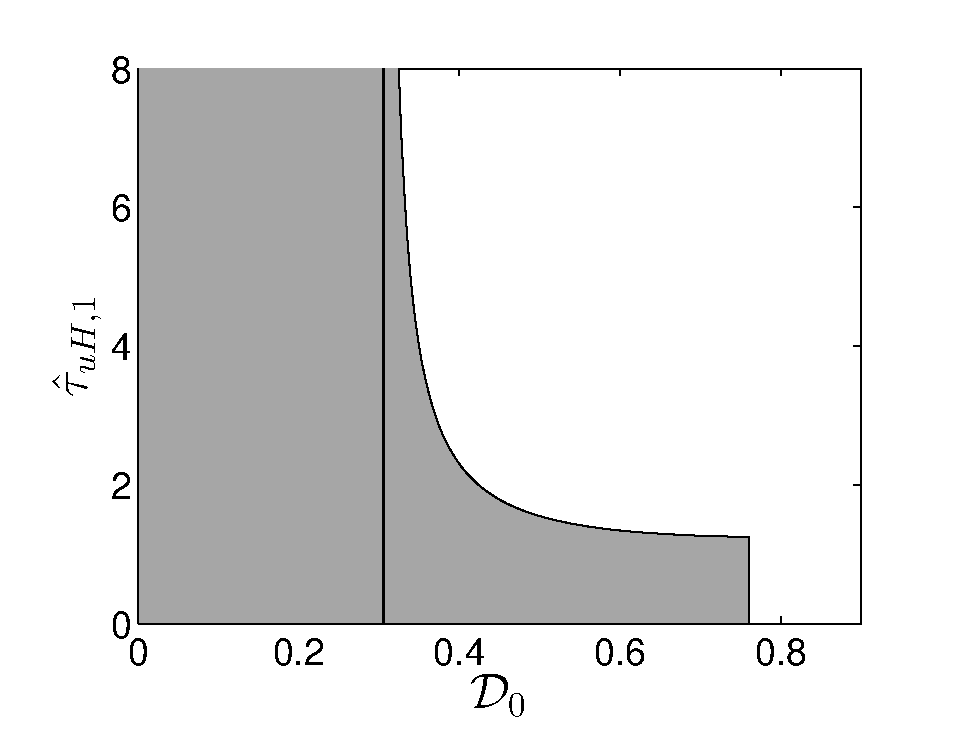
\includegraphics[width=9cm,height=4.8cm]{figs/hopf_2_u02.eps}
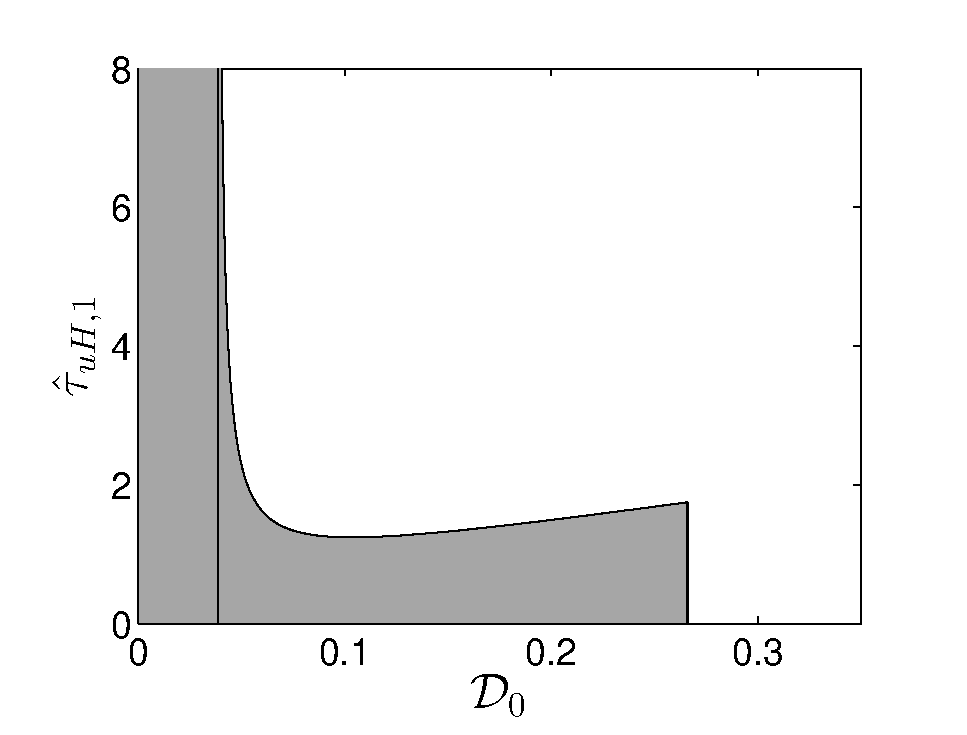
\includegraphics[width=9cm,height=4.8cm]{figs/hopf_2_u04.eps}
\caption{\label{fig:hopf_tau_2} The Hopf bifurcation threshold
  $\hat{\tau}_{uH_1}$ versus ${\mathcal D}_0$ on the range ${{\mathcal
      D}_{0,c}/(1+{3U_0/\omega})}<{\mathcal D}_0<{\mathcal D}_{0c}$
  for $K=2$, $q=3$, $S=6$, $\gamma=2$, $\alpha=1$, for $U_0=2$
  (left panel) and $U_0=4$ (right panel). The two-hotspot pattern is
  linearly stable in the shaded region. The thin
  vertical line in each figure is the lower boundary ${{\mathcal
      D}_{0,c}/(1+{3U_0/\omega})}$, while the right edge of the shaded
  region is the competition stability threshold.  The Hopf bifurcation
  curve in the right panel is not monotonic since
  $U_0>{S(\gamma-\alpha)/(1+\sqrt{3})}$ when $U_0=4$.}
\end{figure}

\begin{cor}\label{q3:main_twospots_pol} Under the conditions of
Proposition \ref{q3:main_twospots} we have the following:
\begin{itemize}
  \item For ${\mathcal D}_0>{\mathcal D}_{0,c} \equiv {S\omega^3
    \left(1+{3U_0/\omega}\right)/[128\pi^2\alpha^2]}$, the two-hotspot
    steady-state is unstable for all scaled police diffusivities $\epsilon^2
    D_p>0$.
 \item On the range ${{\mathcal D}_{0,c}/\left(1+{3U_0/\omega}\right)}
   < {\mathcal D}_0 <{\mathcal D}_{0,c}$, the two hotspot
   steady-state is unstable to an asynchronous oscillatory instability
   of the hotspot amplitudes if $\epsilon^2 D_p<{{\mathcal
       D}_{0}/\hat{\tau}_{uH,1}}$, while the steady-state is linearly
   stable when $\epsilon^2 D_p>{{\mathcal
       D}_{0}/\hat{\tau}_{uH,1}}$. Here $\hat{\tau}_{uH,1}$ is the
   Hopf bifurcation threshold in (\ref{q3:2osc}).
\item On the range $0<{\mathcal D}_0 < {{\mathcal
    D}_{0,c}/\left(1+{3U_0/\omega}\right)}$, the two-hotspot
  steady-state is linearly stable for all $\epsilon^2 D_p\geq 0$.
\end{itemize}
\end{cor}

We now illustrate our main stability results for $K=2$, $S=6$,
$\gamma=2$, and $\alpha=1$. In Fig.~\ref{fig:hopf_tau_2} we plot the
region of linear stability in the $\hat{\tau}_u$ versus ${\mathcal
  D}_0$ parameter plane for $U_0=2$ (left panel) and $U_0=4$ (right
panel). For $U_0=4$, we have $\omega<\sqrt{3}U_0$, and so the Hopf
bifurcation threshold $\hat{\tau}_{uH,1}$ is not monotone in
${\mathcal D}_0$, as seen in the right panel of
Fig.~\ref{fig:hopf_tau_2}. From this figure, we observe that as $U_0$
increases the region where the two-hotspot steady-state is linearly
stable is smaller, as expected. With regards to the scaled police
diffusivity $\epsilon^2 D_p\equiv {{\mathcal D}_0/\hat{\tau}_u}$, in
the right panels of Fig.~\ref{fig:hopf_pol_intro} and
Fig.~\ref{fig:hopf_pol_2} we plot the corresponding region of linear
stability in the $\epsilon^2 D_p$ versus ${\mathcal D}_{0}$ plane for
$U_0=2$ and $U_0=4$, respectively. For $U_0=2$ and $U_0=4$, the
corresponding steady-state two-hotspot solution is shown in the left
panels of Fig.~\ref{fig:hopf_pol_intro} and Fig.~\ref{fig:hopf_pol_2}.
For $U_0=2$, the predicted linear stability results were validated in
Fig.~\ref{fig:valid_2spot_q3} by performing full numerical
solutions of the PDE system (\ref{eq:pol-main}). 

\begin{figure}[htbp]
\centering
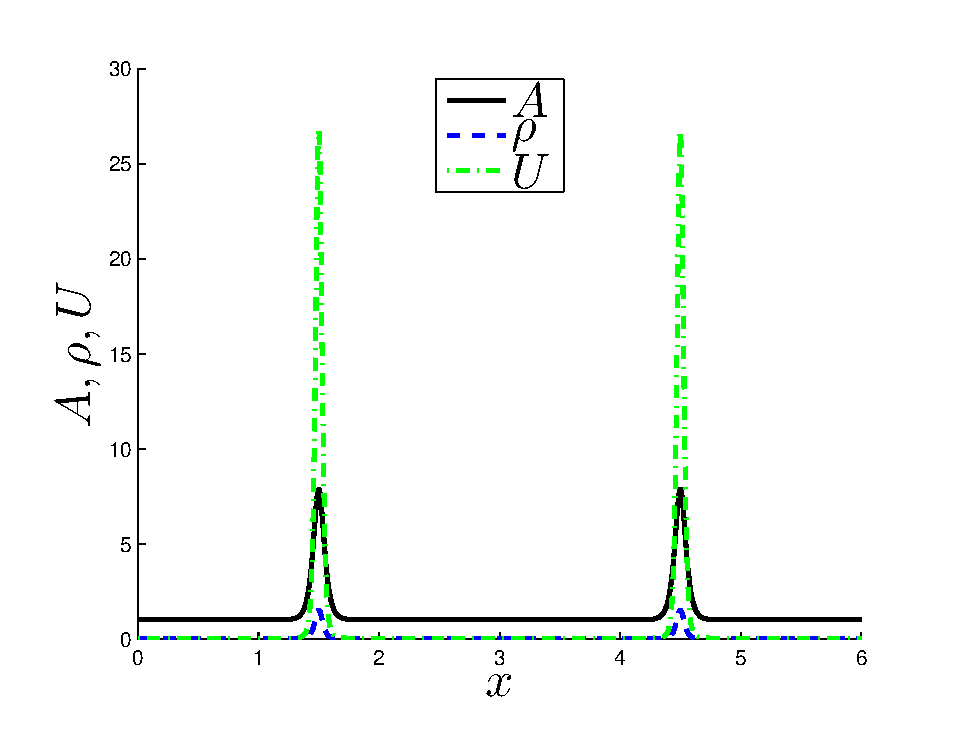
\includegraphics[width=9cm,height=4.8cm]{figs/ss_2_pol_u04.eps}
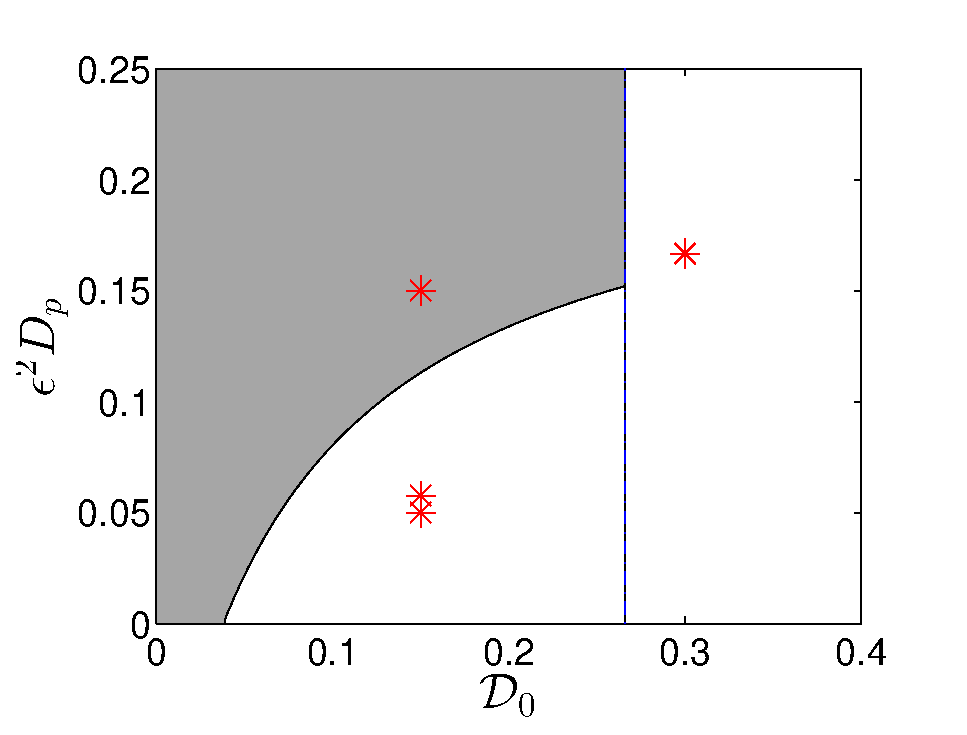
\includegraphics[width=9cm,height=4.8cm]{figs/hopf_2_pol_u04.eps}
\caption{\label{fig:hopf_pol_2} Left panel: the steady-state
  two-hotspot solution for $S=6$, $\gamma=2$, $\alpha=1$, $U_0=4$,
  ${\mathcal D}_0=0.15$, $\epsilon=0.035$, and $q=3$. Right panel:
  Plot of the Hopf bifurcation threshold for the scaled police
  diffusivity $\epsilon^{2}D_p\equiv {{\mathcal
      D}_0/\hat{\tau}_{uH_1}}$ versus ${\mathcal D}_0$ on the range
  ${{\mathcal D}_{0,c}/(1+{3U_0/\omega})} <{\mathcal D}_0<{\mathcal
    D}_{0c}$. The thin vertical line is the competition stability
  threshold ${\mathcal D}_{0,c}$ given in Proposition
  \ref{q3:main_twospots}. The shaded region is where the steady-state
  two-hotspot pattern is linearly stable. For ${\mathcal
    D}_0>{\mathcal D}_{0c}$ the hotspot solution is unstable due to a
  competition instability, whereas in the small unshaded region for
  ${\mathcal D}_0<{\mathcal D}_{0c}$, the hotspot steady-state is
  unstable to an asynchronous oscillatory instability of the hotspot
  amplitudes. The full PDE simulations in
  Fig.~\ref{fig:valid_2_q3_u04} and in Fig.~\ref{fig:valid_2_q3_u04_b}
  are done at the marked points.}
\end{figure}




\subsection{The Stability Phase Diagram for $q=3$: $K\geq 3$ Hotspots}
\label{sect:q3_phase}

Next, we determine the parameter range of ${\mathcal D}_0$ and
$\hat{\tau}_u$ for which a $K$-hotspot steady-state solution, with
$K\geq 3$, is linearly stable. To do so, we need to guarantee that
$\mbox{Re}(\lambda)<0$ for each of the quadratics in
(\ref{stab:q3_quad}), i.e.~for each $j=1,\ldots,K-1$. In this way, we will
ensure that any discrete eigenvalue of the NLEP
(\ref{stab:nlep_final_1}) satisfies $\mbox{Re}(\lambda)\leq 0$.

By using (\ref{q3:interval_1}), we readily obtain the ordering principle that
\begin{equation}\label{q3:d_order}
    D^{\pm}_{0,j+1} < D^{\pm}_{0,j} \,, \quad \mbox{and} \quad
    D^{-}_{0,j} < D^{+}_{0,j} \,, \qquad \mbox{for} \quad j=1,\ldots,K-2 \,.
\end{equation}
We conclude that 
\begin{equation}\label{q3:d_order_1}
    D^{+}_{0,K-1} = \min_{j=1,\ldots,K-1} \lbrace{ D^{+}_{0,j} \rbrace} \,,
    \qquad 
    D^{-}_{0,K-1} = \min_{j=1,\ldots,K-1} \lbrace{ D^{-}_{0,j} \rbrace} \,.
\end{equation}
From Proposition \ref{q3:roots_quad}, we conclude for each of the
quadratics (\ref{stab:q3_quad}), i.e.~for each $j=1,\ldots,K-1$, that
$\mbox{Re}(\lambda)<0$ for any $\hat{\tau}_u\geq 0$ when ${\mathcal
  D}_0<D^{-}_{0,K-1}$. Therefore, a $K$-hotspot steady-state pattern
is linearly stable for all $\hat{\tau}_u\geq 0$ on the range
$0<{\mathcal D}_0<D^{-}_{0,K-1}$. For the range ${\mathcal
  D}_0>D^{+}_{0,K-1}$, we conclude from Proposition
\ref{q3:roots_quad} that the $K-1$ mode must be unstable due to a
positive real eigenvalue for any $\hat{\tau}_u\geq 0$.  Therefore, for
${\mathcal D}_0>D^{+}_{0,K-1}$, a $K$-hotspot steady-state solution is
unstable for all $\hat{\tau}_u\geq 0$.  Additional unstable
eigenvalues due to Hopf bifurcations associated with the remaining modes
$j=1,\ldots,K-2$ are possible depending on the value of
$\hat{\tau}_u$.

To complete the stability phase diagram in the $\hat{\tau}_u$ versus 
${\mathcal D}_0$ parameter plane, we need only focus on the interval
$D^{-}_{0,K-1}<{\mathcal D}_0<D^{+}_{0,K-1}$ where the 
sign-alternating $K-1$ mode undergoes a Hopf bifurcation at 
$\hat{\tau}_u=\hat{\tau}_{uH,K-1}$, given from (\ref{q3:hopf}) by
\begin{equation}\label{q3:hopf_K-1}
     \hat{\tau}_{uH,K-1} \equiv {\mathcal H}\left(\beta\right) \,,
     \qquad \mbox{on} \quad 1\leq \beta \leq
     \frac{D^{+}_{0,K-1}}{D^{-}_{0,K-1}} = 1+ \frac{3U_0}{\omega} \,,
     \qquad \mbox{where} \quad \beta \equiv \frac{{\mathcal
         D}_0}{D^{-}_{0,K-1}} \,.
\end{equation}
Here ${\mathcal H}(\beta)$ is defined in (\ref{q3:h}).  The $K-1$ mode
is linearly stable if and only if $\hat{\tau}_u<\hat{\tau}_{uH,K-1}$.

We now seek to determine conditions for which the Hopf bifurcation
threshold for the $K-1$ mode is smaller than any of the other
$K-2$ possible Hopf bifurcation values $\hat{\tau}_{uH,j}$ for
$j=1,\ldots,K-2$ when restricted to the interval
$D^{-}_{0,K-1}<{\mathcal D}_0<D^{+}_{0,K-1}$. From (\ref{q3:hopf}),
these other Hopf bifurcation thresholds, for $j=1,\ldots,K-2$, can be
written in terms of $\beta$, as defined in (\ref{q3:hopf_K-1}), by
\bsub \label{q3:hopf_jall}
\begin{equation}\label{q3:hopf_j}
    \hat{\tau}_{uH,j} = {\mathcal H}(\xi_j\beta) \,, \qquad \mbox{on}\quad
  \frac{1}{\xi_j} \leq \beta \leq \frac{1}{\xi_j}\left(1 + \frac{3U_0}{\omega}
  \right) \,,
\end{equation}
where, from (\ref{q3:interval}), we define
\begin{equation}\label{q3:hopf_jxi}
 \xi_j \equiv \frac{D^{-}_{0,K-1}}{D^{-}_{0,j}} = \frac{1- \cos\left({\pi j/K}
  \right)}{1 + \cos\left({\pi /K}\right)} \,, \qquad j=1,\ldots,K-2\,.
\end{equation}
We observe from (\ref{q3:hopf_jxi}) that the following ordering
principle holds:
\begin{equation}\label{q3:xi_ord}
   \xi_{j}<\xi_{j+1} <1 \,, \qquad
  j=1,\ldots,K-3 \,, \qquad \xi_{K-2} = \max_{j=1,\ldots,K-2}
  \lbrace{\xi_j\rbrace}\,.
\end{equation}
\esub

Comparing the intervals in (\ref{q3:hopf_j}) and (\ref{q3:hopf_K-1}),
we want to determine a specific parameter range of the total police
deployment $U_0$ for which, for any $j=1,\ldots,K-2$, we have that
$\hat{\tau}_{uH,K-1}<\hat{\tau}_{uH,j}$ on the overlap domain
$\xi_j^{-1}\leq \beta \leq 1+{3U_0/\omega}$. If the overlap domain is
the null-set for the $j$-th mode, i.e.~if
$\xi_j<{1/(1+{3U_0/\omega})}$, then we can simply ignore the $j$-th
mode on $D^{-}_{0,K-1}<{\mathcal D}_0<D^{+}_{0,K-1}$. As such, we need
only consider values of $j$ (if any) for which $\xi_j^{-1} <
1+{3U_0/\omega}$, so that an overlap domain exists. Since ${\mathcal
  H}(\beta)$ is monotone decreasing on $1<\beta<1+\sqrt{3}$, we
readily obtain that ${\mathcal H}(\beta)-{\mathcal
  H}(\xi_j\beta)\equiv \int_{\xi_j\beta}^{\beta} {\mathcal
  H}^{\prime}(y) \, dy <0$ on the interval
$\xi_j^{-1}<\beta<1+\sqrt{3}$. In this way, we conclude that
\begin{equation}\label{q3:hineq}
  {\mathcal H}(\xi_j\beta) < {\mathcal H}(\beta) \,, \qquad \mbox{on}
  \quad \xi_j^{-1}\leq \beta \leq 1 + \frac{3U_0}{\omega} \,, \qquad
  \mbox{when} \quad \omega > \sqrt{3} U_0 \,.
\end{equation}
Therefore, on the range for which ${\mathcal H}(\beta)$ is
monotonically decreasing, it follows that the Hopf bifurcation
threshold of $\hat{\tau}_u$ for any mode $j=1,\ldots,K-2$ cannot be
smaller than that for the $K-1$ mode.  Although the monotonicity of
${\mathcal H}(\beta)$ on $\xi_j^{-1}\leq \beta\leq 1+{3U_0/\omega}$
for $\omega>\sqrt{3}U_0$ provides a sufficient condition for the
ordering principle $\hat{\tau}_{uH,K-1}<\hat{\tau}_{uH,j}$ for
$j=1,\ldots,K-2$ to hold, we now show explicitly that the monotonicity
of ${\mathcal H}(\beta)$ is not strictly necessary.

We now determine a precise condition that ensures that
$\hat{\tau}_{uH,K-1}<\hat{\tau}_{uH,K-2}$ on an assumed overlap domain
$\xi_{K-2}^{-1}\leq \beta \leq 1+{3U_0/\omega}$. Owing to the ordering
principle $\xi_{j}<\xi_{j+1}$ for $j=1,\ldots,K-3$ from
(\ref{q3:xi_ord}), the first Hopf threshold to potentially decrease
below that of the $K-1$ mode must be the $K-2$ mode, and so we focus
only on a comparison with the $K-2$ mode. From (\ref{q3:hopf_K-1}) and
(\ref{q3:hopf_j}), and by using the explicit expression for ${\mathcal
  H}(\beta)$ in (\ref{q3:h}), we calculate after some algebra that
${\mathcal H}(\xi_{K-2}\beta)\geq {\mathcal H}(\beta)$ on
$\xi_{K-2}^{-1}\leq \beta\leq 1+{3U_0/\omega}$, if and only if
\begin{equation}\label{q3:swit_1}
   {\mathcal K}(\beta) \equiv \left(\xi_{K-2}\beta -1\right)(\beta-1)<3
\,, \qquad \mbox{on} \quad 1<\xi_{K-2}^{-1}\leq \beta\leq 1+{3U_0/\omega}\,.
\end{equation}
Since ${\mathcal K}^{\prime}(\beta)>0$ on this interval, this inequality
holds if and only if $1+{3U_0/\omega}<\beta_{\max}$, where
${\mathcal  K}(\beta_{\max})=3$. By setting ${\mathcal K}(\beta)=3$, and
solving the quadratic for $\beta=\beta_{\max}$,
we obtain that (\ref{q3:swit_1}) holds if and only if
\begin{equation}\label{q3:key_swit}
     \frac{\sqrt{3}U_0}{\omega} < {\mathcal Z}(\xi_{K-2}) \,, \qquad
     \mbox{where} \quad {\mathcal Z}(\xi_{K-2}) \equiv
     \frac{1}{\sqrt{3}} \left( -\frac{1}{2} + \frac{1}{2\xi_{K-2}}
       \left[1 + \sqrt{\xi^2_{K-2}+10 \xi_{K-2}+1} \right] \right) \,.
\end{equation}
Here $\omega=S(\gamma-\alpha)-U_0$ and $\xi_{K-2}$ can be found from
(\ref{q3:hopf_jxi}). On $0<\xi<1$, we have that ${\mathcal Z}(\xi)$ 
satisfies
\begin{equation}\label{q:zprop}
   {\mathcal Z}(\xi)\to +\infty \quad \mbox{as} \quad \xi\to 0^{+} \,,
\qquad {\mathcal Z}(1)=1\,, \qquad {\mathcal Z}^{\prime}(\xi)<0 \,, \quad
  \mbox{on} \quad 0<\xi<1 \,.
\end{equation}
It follows that ${\mathcal Z}(\xi)>1$ on $0<\xi<1$. The key inequality
(\ref{q3:key_swit}) implies that $\omega>{\sqrt{3}U_0/{\mathcal
    Z}(\xi_{K-2})}$, which yields a larger range of $\omega$ than the
range $\omega>\sqrt{3}U_0$ where ${\mathcal H}(\beta)$ is monotonic.
This inequality (\ref{q3:key_swit}) can also be used to give a precise
upper bound on $U_0$ for which the $K-1$ mode determines the Hopf
bifurcation threshold for $\hat{\tau}_u$ on the entire range
$D^{-}_{0,K-1}<{\mathcal D}_0<D^{+}_{0,K-1}$. In this way, for $K\geq 3$,
we summarize our main stability result for a $K$-hotspot steady-state 
solution as follows:

\begin{prop}\label{q3:main_Kspots} For $\epsilon\to 0$, 
$q=3$, $K\geq 3$, $0<U_0<U_{0,\max}$, $\hat{\tau}_u\ll
  {\mathcal O}(\epsilon^{-2})$, and ${\mathcal D}_0=\epsilon^2 D =
  {\mathcal O}(1)$, the linear stability properties of a $K$-hotspot
  steady-state solution of (\ref{eq:pol-main}) are as follows:
\begin{itemize}
  \item For ${\mathcal D}_0>D^{+}_{0,K-1} \equiv {\mathcal D}_{0,c}$, the
    NLEP (\ref{stab:nlep_final_1}) has at least one positive real eigenvalue for
    all $\hat{\tau}_u\geq 0$. Additional unstable eigenvalues as a result
    of Hopf bifurcations associated with the other modes $j=1,\ldots,K-2$ 
    are possible  depending on the value of $\hat{\tau}_u$. Here 
    ${\mathcal D}_{0,c}$ is the competition stability threshold given in
    (\ref{stab:zero_d0min}) with $q=3$.
 \item On the range $D^{-}_{0,K-1} \equiv 
  {{\mathcal D}_{0,c}/\left(1+{3U_0/\omega}\right)} < {\mathcal D}_0
    <{\mathcal D}_{0,c}$, and when $U_0$ satisfies
\begin{equation}\label{q3:u0mon}
     U_0 < U_{0,\textrm{swit}} \equiv \left( \frac{ {\mathcal Z}(\xi_{K-2})}
  { \sqrt{3} + {\mathcal Z}(\xi_{K-2})} \right) \, S(\gamma-\alpha)
  \,, \qquad \mbox{where} \quad \xi_{K-2} \equiv 
  \frac{1- \cos\left({\pi (K-2)/K}\right)}{1 + \cos\left({\pi /K}\right)} \,, 
\end{equation}
and where ${\mathcal Z}(\xi)$ is defined in (\ref{q3:key_swit}), the
$K-1$ sign-alternating mode sets the stability threshold on the entire
range.  For $\hat{\tau}_u>\hat{\tau}_{uH,K-1}$, the $K$-hotspot
pattern is unstable, while if $\hat{\tau}_u<\hat{\tau}_{uH,K-1}$ the
$K$-hotspot pattern is linearly stable. With ${\mathcal H}(\beta)$, as
defined in (\ref{q3:h}), the minimal Hopf bifurcation value of
$\hat{\tau}_u$ is 
\begin{equation}\label{q3:Kosc}
 \hat{\tau}_{uH,K-1}\equiv {\mathcal H}\left({{\mathcal
     D}_0/D^{-}_{0,K-1}}\right) \,, \quad \mbox{on} \quad
 D^{-}_{0,K-1}\equiv \frac{{\mathcal D}_{0c}}{1+{3U_0/\omega}}<{\mathcal
   D}_0 <{\mathcal D}_{0,c} \,,
\end{equation}
where 
\item On the range $0<{\mathcal D}_0 < D^{-}_{0,K-1} \equiv {{\mathcal
    D}_{0,c}/\left(1+{3U_0/\omega}\right)}$, the $K$-hotspot
  steady-state is linearly stable for all $\hat{\tau}_u\geq 0$.
\end{itemize}
\end{prop}

\noindent In terms of a scaled police diffusivity defined by 
$\epsilon^2 D_p\equiv {{\mathcal D}_0/\hat{\tau}_u}$, Proposition
\ref{q3:main_Kspots} implies the following:

\begin{cor}\label{q3:main_Kspots_pol} Under the conditions of
Proposition \ref{q3:main_Kspots}, we have the following:
\begin{itemize}
  \item For ${\mathcal D}_0>{\mathcal D}_{0,c}$, the $K$-hotspot
    steady-state is unstable for all scaled police diffusivities $\epsilon^2
    D_p>0$. Here ${\mathcal D}_{0,c}$ is defined in
   (\ref{stab:zero_d0min}) with $q=3$.
 \item On the range ${{\mathcal D}_{0,c}/\left(1+{3U_0/\omega}\right)}
   < {\mathcal D}_0 <{\mathcal D}_{0,c}$, and when $U_0<U_{0,\textrm{swit}}$,
   as defined in (\ref{q3:u0mon}), the $K$-hotspot steady-state is 
  unstable to a sign-alternating asynchronous oscillatory instability
   of the hotspot amplitudes if $\epsilon^2 D_p<{{\mathcal
       D}_{0}/\hat{\tau}_{uH,K-1}}$ where $\hat{\tau}_{uH,K-1}$ is defined in
  (\ref{q3:Kosc}). Alternatively, this steady-state is linearly
   stable when $\epsilon^2 D_p>{{\mathcal
       D}_{0}/\hat{\tau}_{uH,K-1}}$.
\item On the range $0<{\mathcal D}_0 < {{\mathcal
    D}_{0,c}/\left(1+{3U_0/\omega}\right)}$, the $K$-hotspot
  steady-state is linearly stable for all $\epsilon^2 D_p\geq 0$.
\end{itemize}
\end{cor}

We remark that the upper bound $U_{0,\textrm{swit}}$ in
(\ref{q3:u0mon}) can be calculated explicitly when $K=3$ and
$K=4$. When $K=3$, we calculate $\xi_1={1/3}$ and ${\mathcal
  Z}(\xi_1)={\left(1+\sqrt{10}\right)/\sqrt{3}}$.  We then obtain from
(\ref{q3:u0mon}) that the sign-alternating $K-1$ mode sets the Hopf
bifurcation threshold when
\begin{equation}\label{q3:U_0swit_3}
    U_0< U_{0,\textrm{swit}} \equiv \frac{3 S(\gamma-\alpha)}{2+\sqrt{10}} \approx
   (0.58114) S(\gamma-\alpha) \,, \qquad \mbox{for} \quad K=3 \,.
\end{equation}
Similarly, for $K=4$, we calculate $\xi_2=2-\sqrt{2}$, and 
\begin{equation*}
   {\mathcal Z}(\xi_2) =\frac{1}{\sqrt{3}}\left[ \frac{\sqrt{2}}{4} +
     \left( \frac{1}{2} + \frac{\sqrt{2}}{4} \right) \sqrt{27 -
       14\sqrt{2}}\right] \approx 1.5265 \,.
\end{equation*}
From (\ref{q3:u0mon}), the $K-1$ mode sets the Hopf bifurcation threshold when
\begin{equation}\label{q3:U_0swit_4}
    U_0< U_{0,\textrm{swit}} \approx (0.46847) S(\gamma-\alpha) \,, \qquad 
\mbox{for} \quad K=4 \,.
\end{equation}

\begin{figure}[htbp]
\centering
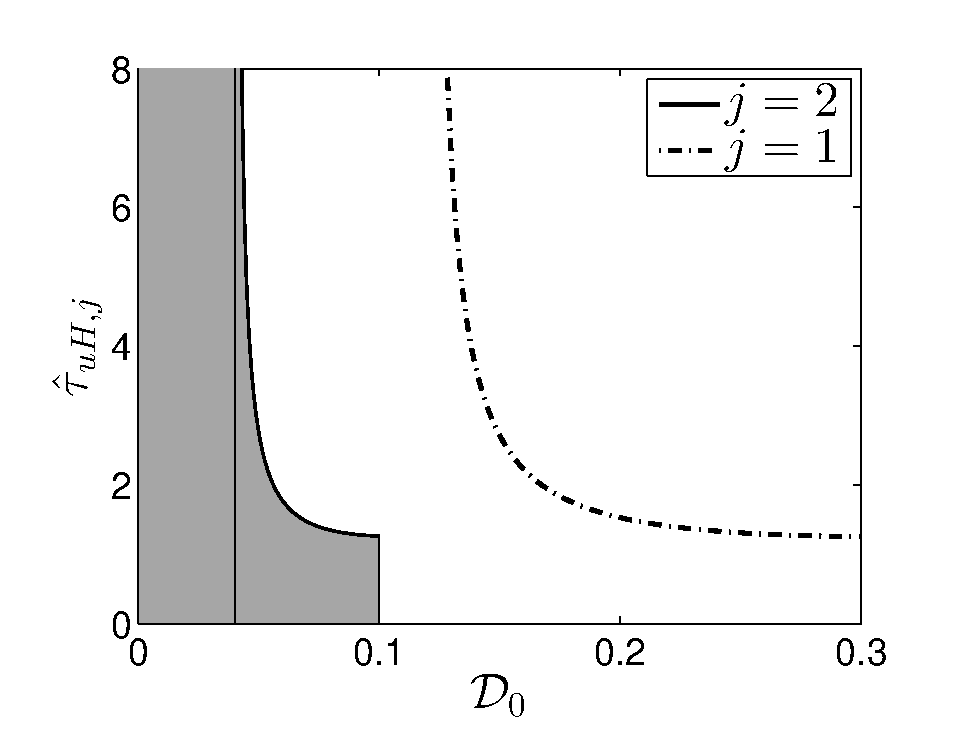
\includegraphics[width=0.47\textwidth,height=4.8cm]{figs/hopf_3_u02.eps}
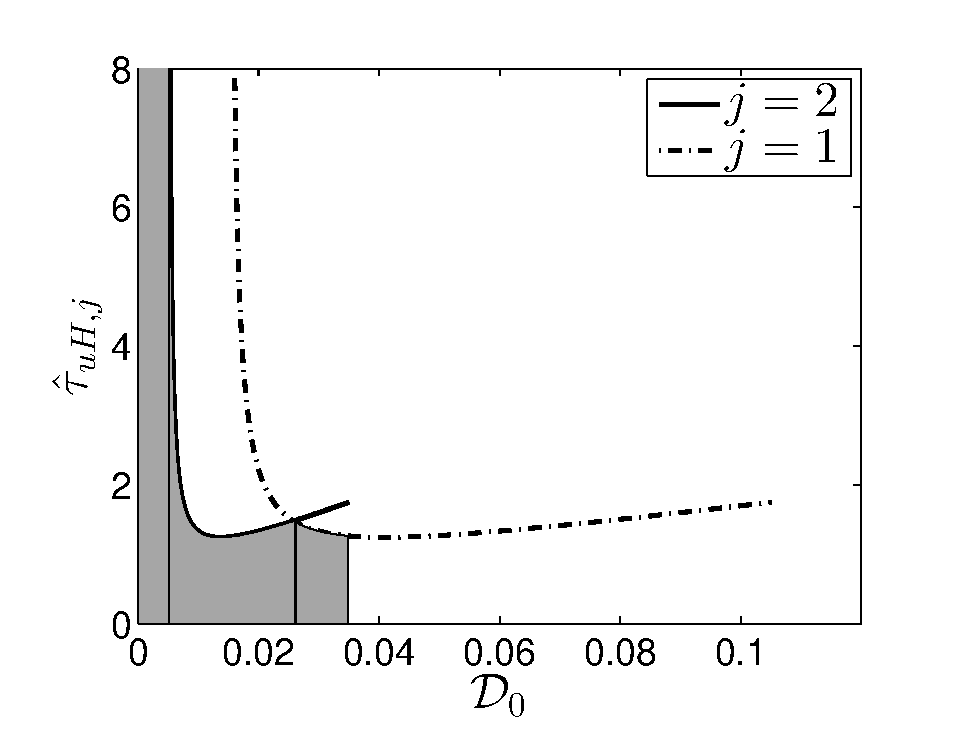
\includegraphics[width=0.47\textwidth,height=4.8cm]{figs/hopf_3_u04.eps}
\caption{\label{fig:hopf_tau_3} Linear stability (shaded) region in
  the $\hat{\tau}_u$ versus ${\mathcal D}_0$ plane for $K=3$ when
  $S=6$, $\gamma=2$, and $\alpha=1$, and for $U_0=2$ (left panel) and
  $U_{0}=4$ (right panel), as characterized by Proposition
  \ref{q3:main_Kspots}. To the left of the thin vertical line the
  steady-state is unconditionally stable. The solid and dot-dashed curves
  are the Hopf bifurcation boundaries for the (sign-alternating) $j=2$
  mode and the $j=1$ mode, respectively. For $U_0=2$ (left panel) the
  Hopf boundary is determined by the $j=2$ mode.  For
  $U_0=4>U_{0,\textrm{swit}}\approx 3.478$ (right panel) the Hopf
  boundary consists of both the $j=2$ and $j=1$ mode. The
  three-hotspot steady-state is unstable to an oscillatory instability
  above the solid or dotted curves. At the ends of the Hopf
  bifurcation curves the Hopf eigenvalue tends to zero.}
\end{figure}


We now illustrate our main stability results in Proposition
\ref{q3:main_Kspots} and Corollary \ref{q3:main_Kspots_pol} for 
$S=6$, $\gamma=2$, and $\alpha=1$. We take $K=3$ or $K=4$, and either
$U_0=2$ and $U_0=4$. For these parameters, (\ref{q3:U_0swit_3}) and
(\ref{q3:U_0swit_4}) yield that $U_{0,\textrm{swit}}\approx 3.487$ for
$K=3$ and $U_{0,\textrm{swit}}\approx 2.811$ for $K=4$. Therefore, for
both $K=3$ and $K=4$ it is only for the smaller value $U_0=2$ that the
sign-alternating mode sets the Hopf bifurcation threshold.

For $K=3$, the shaded region in Fig.~\ref{fig:hopf_tau_3} is the
theoretically predicted region of linear stability in the
$\hat{\tau}_u$ versus ${\mathcal D}_0$ parameter plane for $U_0=2$
(left panel) and for $U_0=4$ (right panel). In this figure the dotted
curve and solid curves are the Hopf bifurcation thresholds for the
$j=1$ mode and the sign-alternating $j=2$ mode. When $U_0=2$ (left
panel), the sign-alternating mode sets the boundary of the region of
stability, whereas for $U_0=4$ (right panel) both the $j=1$ and $j=2$
Hopf bifurcation thresholds form the boundary of the region of
stability. The corresponding region of stability in the scaled police
diffusivity $\epsilon^2 D_p$ versus ${\mathcal D}_0$ parameter plane
is shown in Fig.~\ref{fig:hopf_pol_3}.

\begin{figure}[htbp]
\centering
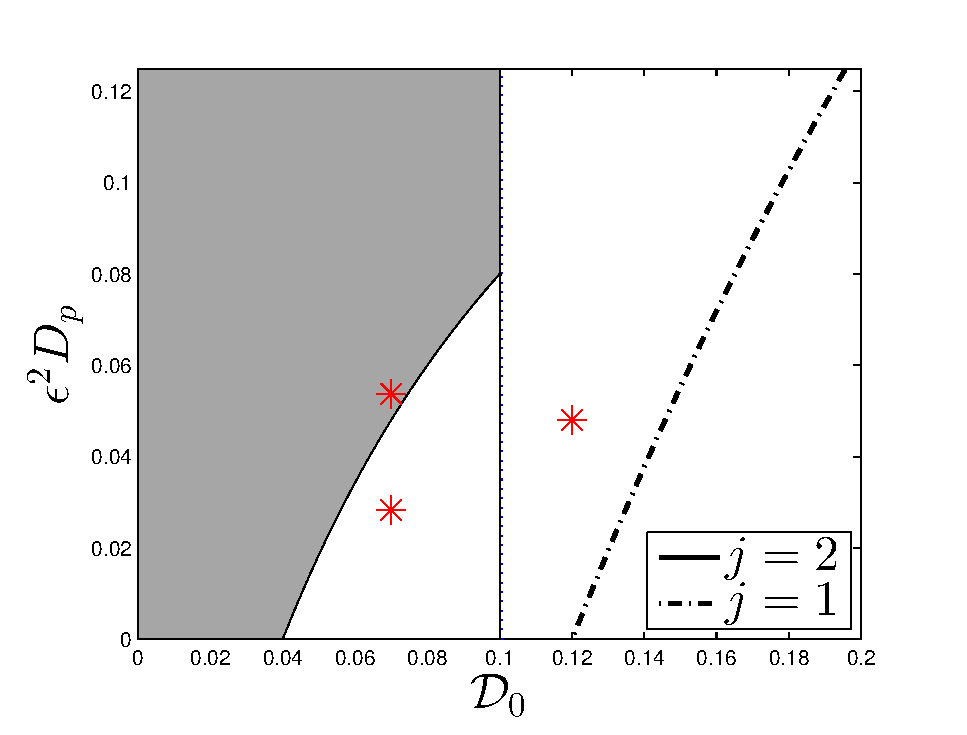
\includegraphics[width=0.47\textwidth,height=4.8cm]{figs/pol_3_u02.eps}
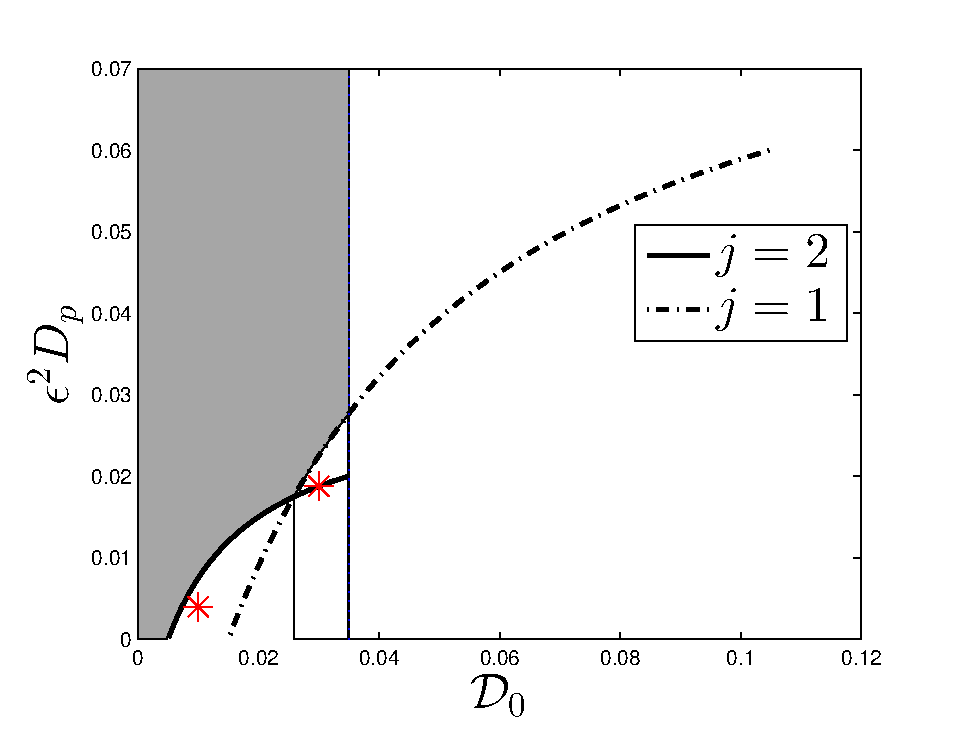
\includegraphics[width=0.47\textwidth,height=4.8cm]{figs/pol_3_u04.eps}
\caption{\label{fig:hopf_pol_3} Same plot as Fig.~\ref{fig:hopf_tau_3}
  except in the scaled police diffusivity $\epsilon^{2}D_p={{\mathcal
      D}_0/\hat{\tau}_u}$ versus ${\mathcal D}_0$ plane for $K=3$,
  $S=6$, $\gamma=2$, and $\alpha=1$, with $U_0=2$ (left panel) and
  $U_{0}=4$ (right panel) (see Corollary
  \ref{q3:main_Kspots_pol}). The three-hotspot steady-state is
  linearly stable in the shaded region. This steady-state undergoes an
  oscillatory instability below the solid or dot-dashed curves. In the
  left panel the thin vertical line is the competition threshold
  ${\mathcal D}_{0,c}$. The additional thin vertical line in the right
  panel is where the Hopf boundary switches from $j=2$ to $j=1$. This
  switch occurs since $U_0=4>U_{0,\textrm{swit}}\approx 3.478$ (see
  (\ref{q3:U_0swit_3}) and the second statement of Corollary
  \ref{q3:main_Kspots_pol}). The full PDE simulations in
  Fig.~\ref{fig:valid_3spot_q3} and in Fig.~\ref{fig:valid_3spot_q3_b}
  are done at the marked points in the left and right panels,
  respectively.}
\end{figure}


Similar results for $K=4$ and for $U_0=2$ and $U_0=4$ are shown in
Fig.~\ref{fig:hopf_tau_4} in the $\hat{\tau}_u$ versus ${\mathcal D}_0$
plane and in Fig.~\ref{fig:hopf_pol_4} in the $\epsilon^2 D_p$ versus
${\mathcal D}_0$ plane. From the left panels of
Fig.~\ref{fig:hopf_tau_4} and Fig.~\ref{fig:hopf_pol_4}, the $j=K-1=3$
sign-alternating mode always sets the Hopf bifurcation boundary. However,
as seen in the right panels of Fig.~\ref{fig:hopf_tau_4} and 
Fig.~\ref{fig:hopf_pol_4}, where $U_0=4>U_{0,\textrm{swit}}\approx 2.811$, we 
observe that both the $j=3$ and $j=2$ modes determine the Hopf bifurcation
boundary when ${\mathcal D}_0<{\mathcal D}_{0,c}$.


\begin{figure}[htbp]
\centering
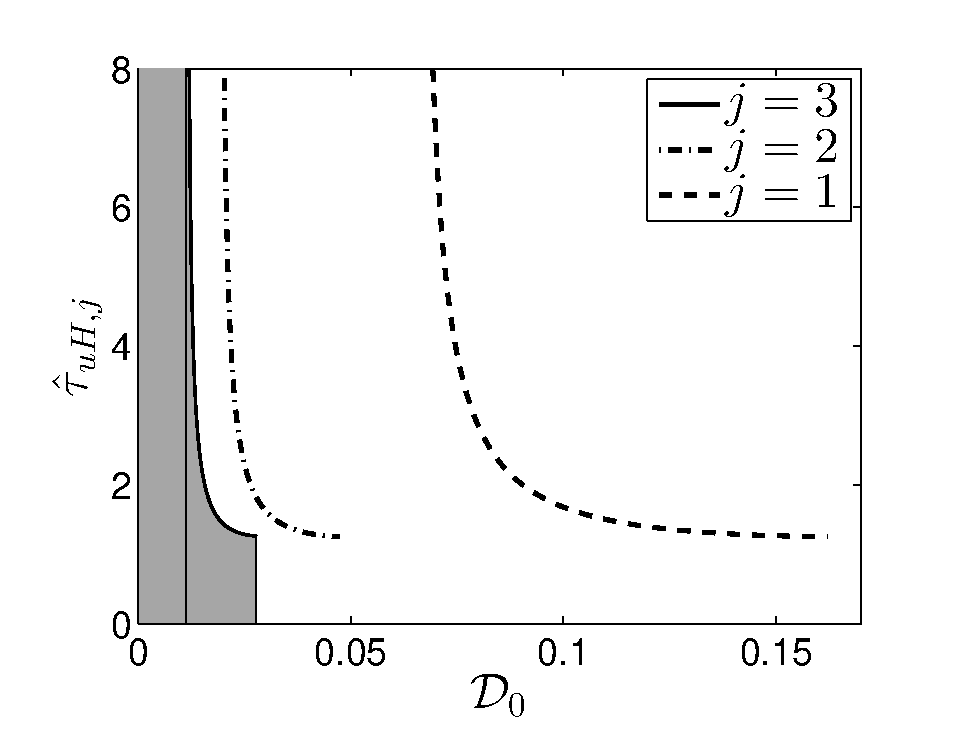
\includegraphics[width=0.47\textwidth,height=4.8cm]{figs/hopf_4_u02.eps}
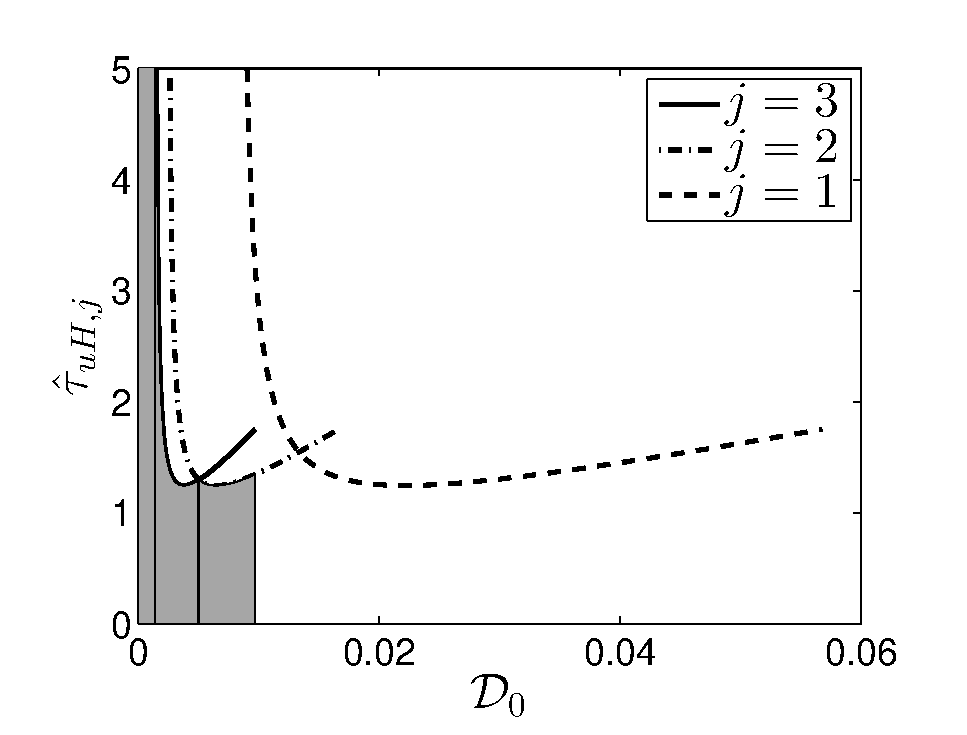
\includegraphics[width=0.47\textwidth,height=4.8cm]{figs/hopf_4_u04.eps}
\caption{\label{fig:hopf_tau_4} Linear stability (shaded) region in
  the $\hat{\tau}_u$ versus ${\mathcal D}_0$ plane for $K=4$ when
  $S=6$, $\gamma=2$, and $\alpha=1$, and for $U_0=2$ (left panel) and
  $U_{0}=4$ (right panel). The solid, dot-dashed, and dashed curves
  are the Hopf bifurcation boundaries for the (sign-alternating) $j=3$
  mode and the other $j=2$ and $j=1$ modes. For $U_0=2$ (left panel)
  the Hopf boundary is determined by the sign-alternating $j=3$ mode.
  For $U_0=4>U_{0,\textrm{swit}}\approx 2.811$ (see
  (\ref{q3:U_0swit_4})), the Hopf boundary consists of both the $j=3$
  and $j=2$ mode. Asynchronous oscillatory instabilities of the
  hotspot amplitudes occur above any of the Hopf bifurcation curves.}
\end{figure}

\begin{rem}
More generally, for $K\geq 3$ there can be $K-2$ distinct mode
switches for the minimal Hopf bifurcation threshold on the interval
$D^{-}_{0,K-1}<{\mathcal D}_0<D^{+}_{0,K-1}$ when $U_0$ increases
beyond $U_{0,\textrm{swit}}$ towards $U_{0,\max}$. Although we do not
work out precise conditions for this {\em cascading behavior} of the
minimal Hopf bifurcation value here, we illustrate this phenomena in
Fig.~\ref{fig:cascade} for $K=4$, $S=6$, $\gamma=2$, $\alpha=1$, and
$U_0=5$. From this figure, we observe two mode switches of the minimal
Hopf bifurcation threshold. This suggests that as $U_0$ approaches the
existence threshold $U_{0,\max}$, there is a window of ${\mathcal
  D}_0$ where $K-2$ distinct modes of oscillatory instability of the
hotspot amplitudes can occur if $\hat{\tau}_u$ is large enough,
suggesting the possibility of intricate spatio-temporal dynamics in
this parameter regime.
\end{rem}

\begin{figure}[htbp]
\centering
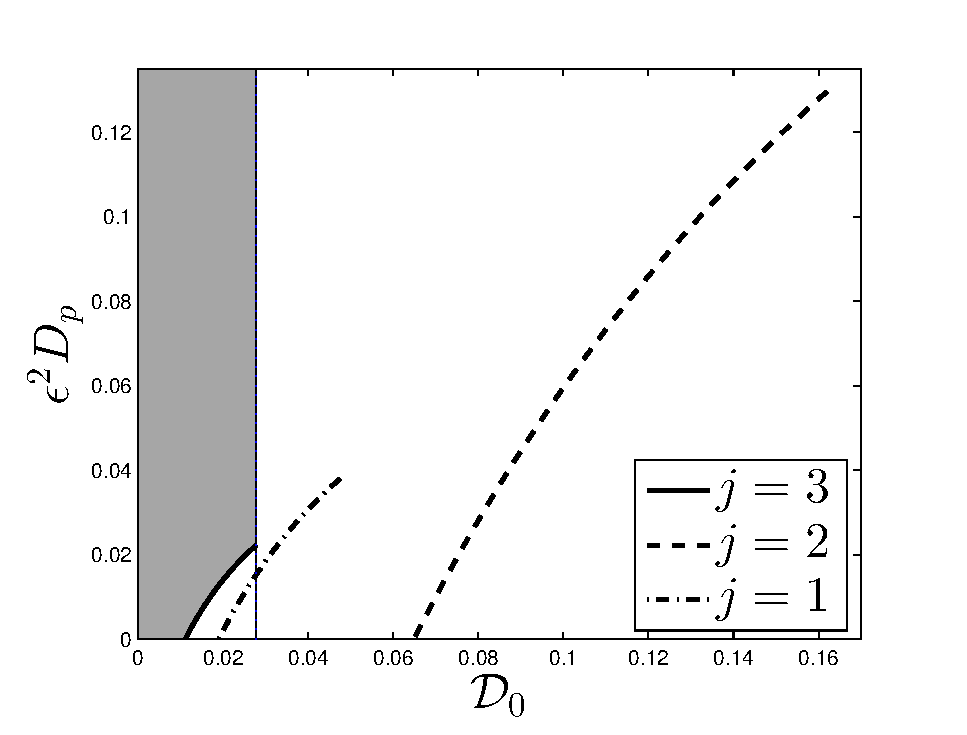
\includegraphics[width=0.47\textwidth,height=4.8cm]{figs/pol_4_u02.eps}
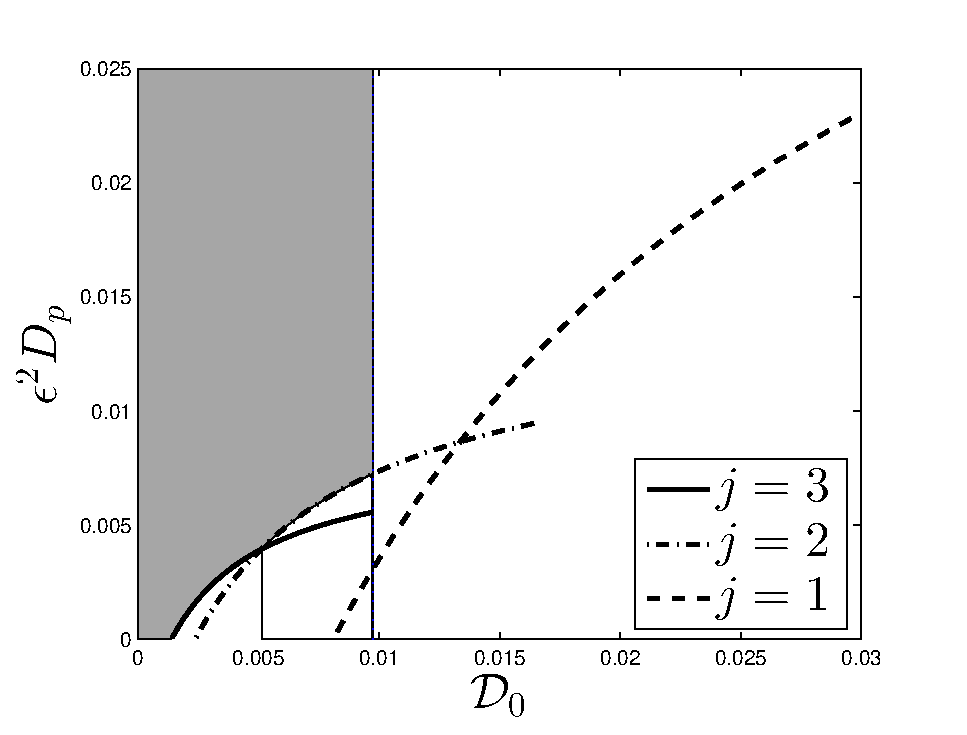
\includegraphics[width=0.47\textwidth,height=4.8cm]{figs/pol_4_u04.eps}
\caption{\label{fig:hopf_pol_4} Plot corresponding to
  Fig.~\ref{fig:hopf_tau_4} in the scaled police diffusivity
  $\epsilon^{2}D_p={{\mathcal D}_0/\hat{\tau}_u}$ versus ${\mathcal
    D}_0$ plane for $K=4$, $S=6$, $\gamma=2$, and $\alpha=1$, with
  $U_0=2$ (left panel) and $U_{0}=4$ (right panel). The four-hotspot
  steady-state is linearly stable in the shaded region. This
  steady-state undergoes an asynchronous oscillatory instability below
  either of the three Hopf bifurcation curves.  In the left panel the
  thin vertical line is the competition threshold ${\mathcal
    D}_{0,c}$. The additional thin vertical line in the right panel is
  where the Hopf boundary switches from $j=3$ to $j=2$. The Hopf
  eigenvalue tends to zero at the ends of each of the two curves.}
\end{figure}

\begin{figure}[htbp]
\centering
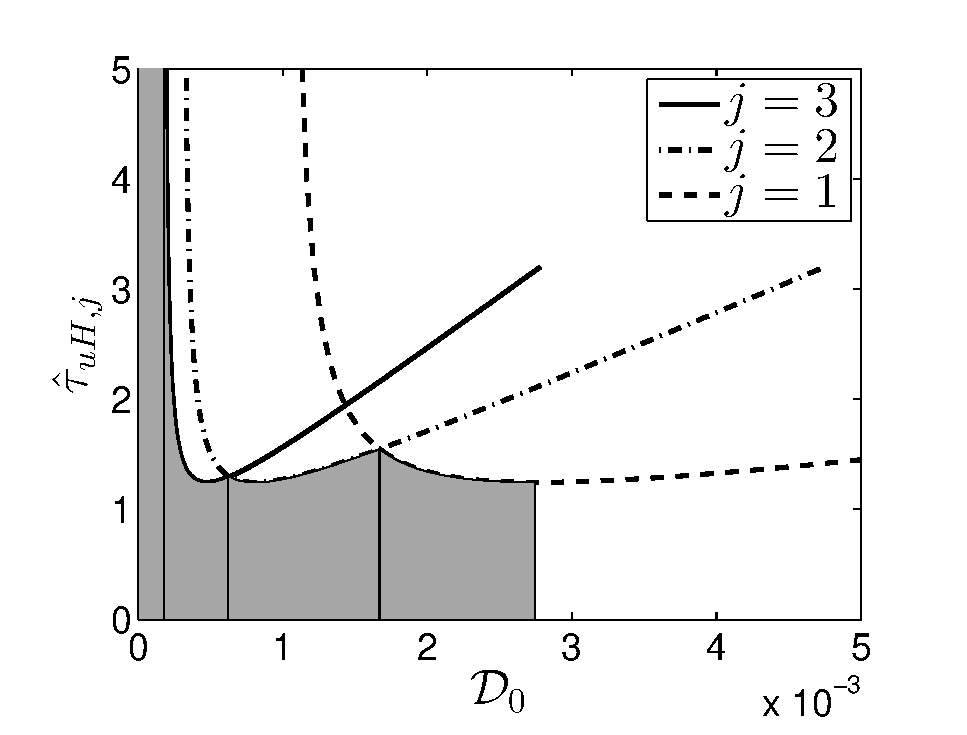
\includegraphics[width=0.50\textwidth,height=4.8cm]{figs/hopf_cascade.eps}
\caption{\label{fig:cascade} Linear stability (shaded) region in the
  $\hat{\tau}_u$ versus ${\mathcal D}_0$ plane for $K=4$ when $S=6$,
  $\gamma=2$, and $\alpha=1$, and for $U_0=5$. The solid, dot-dashed,
  and dashed curves are the Hopf bifurcation boundaries for the
  (sign-alternating) $j=3$ mode, the $j=2$ mode, and the $j=1$ mode,
  respectively. Notice that the minimal Hopf bifurcation threshold on
  $D^{-}_{0,K-1}<{\mathcal D}_0<D^{+}_{0,K-1}$ now consists of all
  three modes. Asynchronous oscillatory instabilities of the hotspot
  amplitudes occur above either of the three Hopf bifurcation curves.}
\end{figure}


\subsection{Comparison of Linear Stability Theory with PDE Simulations: $q=3$}
\label{sec:numerics_q3}

For various points in the stability phase diagrams of $\epsilon^2 D_p$
versus ${\mathcal D}_0$, we now confirm our linear stability
predictions by performing full numerical simulations of the RD system
(\ref{eq:pol-main}) using the collocation-based 1-D VLUGR \cite{vlug}
software, which uses adaptive meshing and error controlled
time-stepping. For the initial condition for (\ref{eq:pol-main}) we
use a slightly smoothed approximation to a $K$-hotspot steady-state
solution, as given in Corollary \ref{cor:pol-K-hotspots-in-A-rho-U},
with the explicit form 
\bsub \label{comp:ic}
\begin{gather}
  A(x,0) = \frac{1}{\sigma \sqrt{v_0}} \sum_{j=1}^{K} \left(1+0.01 a_j\right) 
    w\left[\sigma^{-1}(x-x_j)\right] + \alpha \left( 1- \sum_{j=1}^{K}
   e^{-(x-x_j)^2/\sigma^2}\right) \,, \label{comp:ic_1}\\
 \rho(x,0) = \sum_{j=1}^{K} \left( w[\sigma^{-1}(x-x_j)]\right)^2 \,, \qquad
  U(x,0)= \frac{U_0}{\sigma K I_q} \sum_{j=1}^{K}
  \left(w[\sigma^{-1}(x-x_j)]\right)^q \,.
\end{gather}
\esub Here $q=3$ and the hotspot locations are at their steady-state
values $x_j=S(2j-1)/(2K)$ for $j=1,\ldots,K$.  The last term in
(\ref{comp:ic_1}) is used solely to subtract off the baseline
attractiveness from the localized hotspot regions. In
(\ref{comp:ic_1}), the random coefficient $a_j$ of the $1\%$
perturbation of the hotspot amplitudes is taken to be uniformly
distributed in $[-1,1]$. In addition, the smoothing parameter
$\sigma$, taken as $\sigma=1.2\epsilon$, was introduced so as to allow
the time-stepper to converge in the PDE simulations with an initial
uniformly-spaced of $1000$ points on $0<x<S$. For all of the full PDE
simulations reported below, we will display the amplitudes of the maxima
of $A$ versus $t$ for the baseline parameter set $S=6$, $\gamma=2$,
and $\alpha=1$.

\begin{figure}[htbp]
\centering
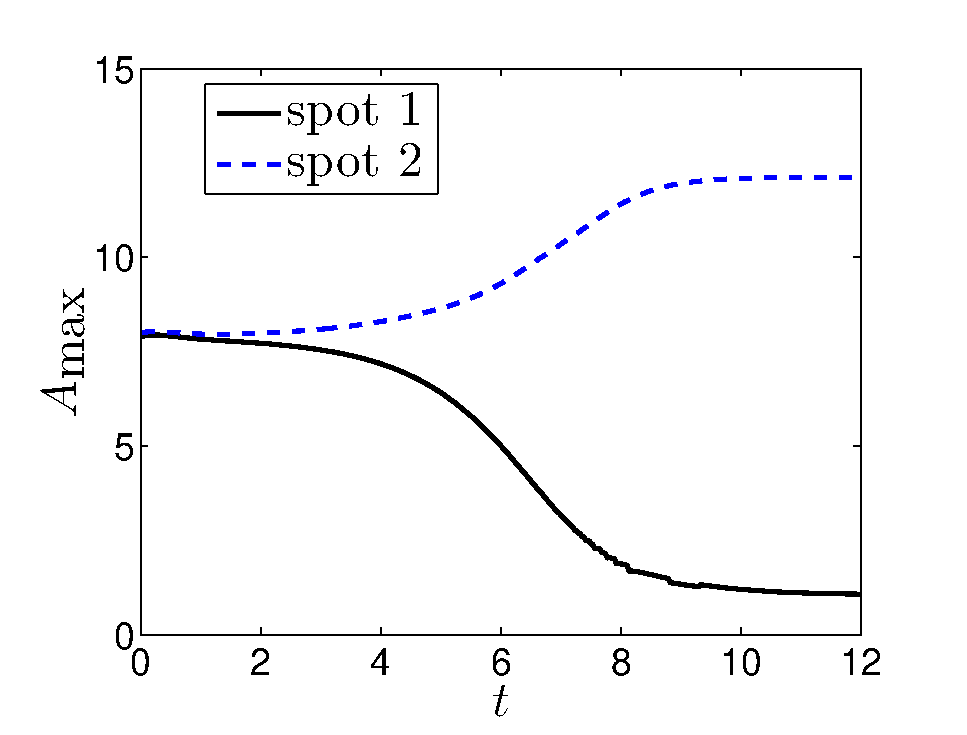
\includegraphics[width=0.47\textwidth,height=4.8cm]{figs/amp_2_run6.eps}
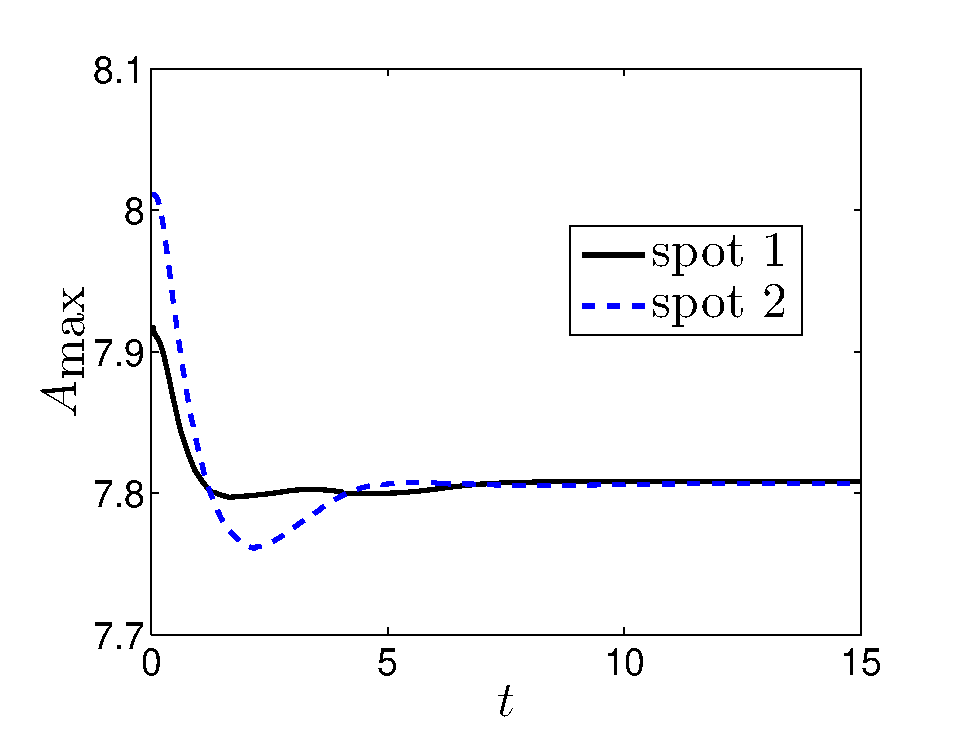
\includegraphics[width=0.47\textwidth,height=4.8cm]{figs/amp_2_run4.eps}
\caption{\label{fig:valid_2_q3_u04} The spot amplitudes
  computed numerically from the full PDE system (\ref{eq:pol-main})
  for a two-spot pattern with $S=6$, $\gamma=2$, $\alpha=1$, $U_0=4$,
  $\epsilon=0.035$, and $q=3$, at two of the marked points in the
  right panel of Fig.~\ref{fig:hopf_pol_2}.  Left panel:
  $\hat{\tau}_u=1.8$ and ${\mathcal D}_0=0.3$, so that $\epsilon^2
  D_p\approx 0.1667$. Spot amplitudes are unstable to a competition
  instability. Right panel: $\hat{\tau}_u=1.0$ and ${\mathcal D}_0=0.15$, so
  that $\epsilon^2D_p = 0.15$. Spot amplitude asynchronous
  oscillations decay in time and there is no competition instability.
  These results are consistent with the linear stability predictions
  in the right panel of Fig.~\ref{fig:hopf_pol_2} (see also the right
  panel of Fig.~\ref{fig:hopf_tau_2}).}
\end{figure}

For a two-hotspot steady-state, in Fig.~\ref{fig:valid_2spot_q3} of \S
\ref{sec:intro} we confirmed the predictions of the three marked
points in the phase diagram in Fig.~\ref{fig:hopf_pol_intro} for
$U_0=2$ and $\epsilon=0.075$. A similar validation of the linear
stability phase diagram in the right panel of
Fig.~\ref{fig:hopf_pol_2} for $U_0=4$, with the smaller value
$\epsilon=0.035$, is given in Fig.~\ref{fig:valid_2_q3_u04} and
Fig.~\ref{fig:valid_2_q3_u04_b}. Our choice of a smaller $\epsilon$
here is due to the fact that the steady-state hotspot amplitude is
considerably smaller for $U_0=4$ than when $U_0=2$. Moreover, in
Fig.~\ref{fig:valid_2_q3_u04_b} we show that for two nearby points in
the phase diagram where an asynchronous oscillatory instability is
predicted, the long-time dynamics can be rather different in that either
one, or both, of the hotspots are ultimately annihilated.

\begin{figure}[htbp]
\centering
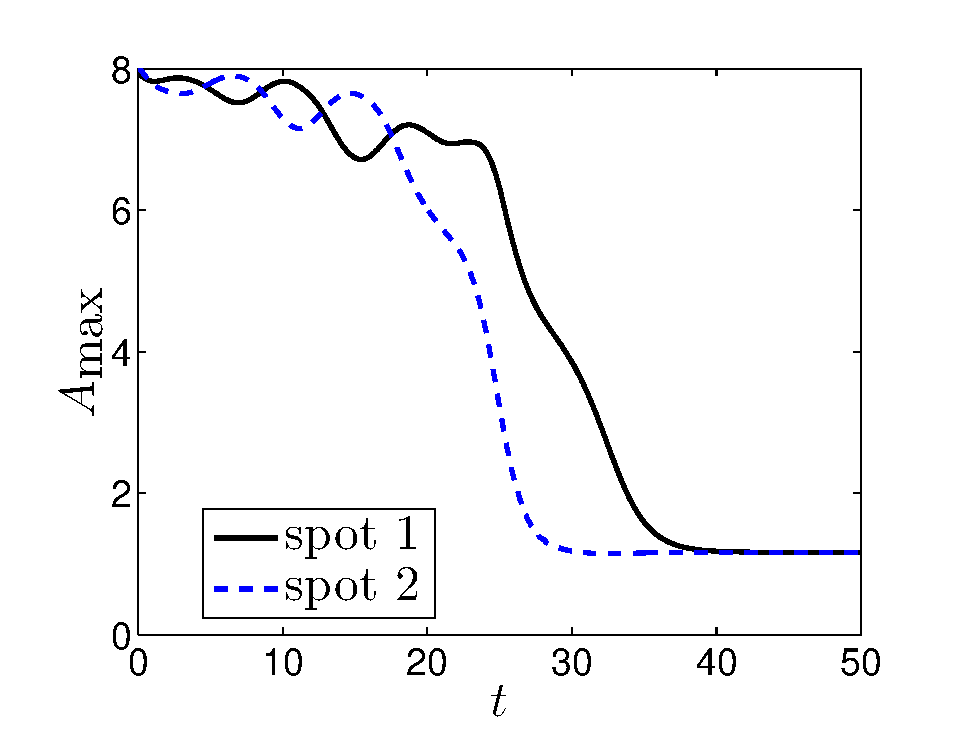
\includegraphics[width=0.47\textwidth,height=4.8cm]{figs/amp_2_run5.eps}
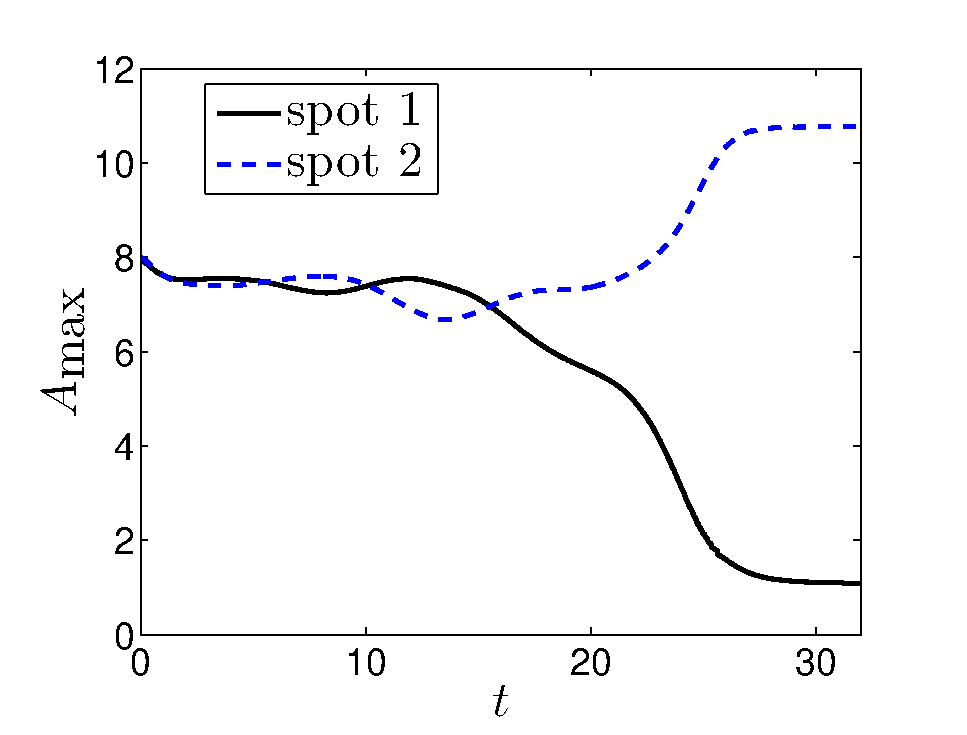
\includegraphics[width=0.47\textwidth,height=4.8cm]{figs/amp_2_run7.eps}
\caption{\label{fig:valid_2_q3_u04_b} The oscillatory
  instabilities of the spot amplitudes computed numerically from the
  full PDE system (\ref{eq:pol-main}) for a two-spot pattern with
  $S=6$, $\gamma=2$, $\alpha=1$, $U_0=4$, $\epsilon=0.035$, and $q=3$,
  at the marked points in the right panel of Fig.~\ref{fig:hopf_pol_2}
  where an oscillatory instability occurs.  Left panel:
  $\hat{\tau}_u=2.6$ and ${\mathcal D}_0=0.15$, so that $\epsilon^2
  D_p\approx 0.0577$. Spot amplitudes are unstable to asynchronous
  oscillations, which leads to the collapse of both hotspots.  Right
  panel: $\hat{\tau}_u=3.0$ and ${\mathcal D}_0=0.15$, so that
  $\epsilon^2 D_p= 0.05$. Spot amplitudes are unstable to asynchronous
  oscillations, but now only one of the two hotspots is annihilated.}
\end{figure}

For a three-hotspot pattern with $\epsilon=0.05$ and $U_0=2$, in
Fig.~\ref{fig:valid_3spot_q3} we show full numerical results, as
computed from (\ref{eq:pol-main}), for the hotspot amplitudes at the
three marked points in the left panel of
Fig.~\ref{fig:hopf_pol_3}. These results are completely consistent
with the prediction of our phase diagram. The middle panel of
Fig.~\ref{fig:valid_3spot_q3} shows that the asynchronous oscillation
is due to the sign-altering mode, as predicted theoretically.

\begin{figure}[htbp]
\centering
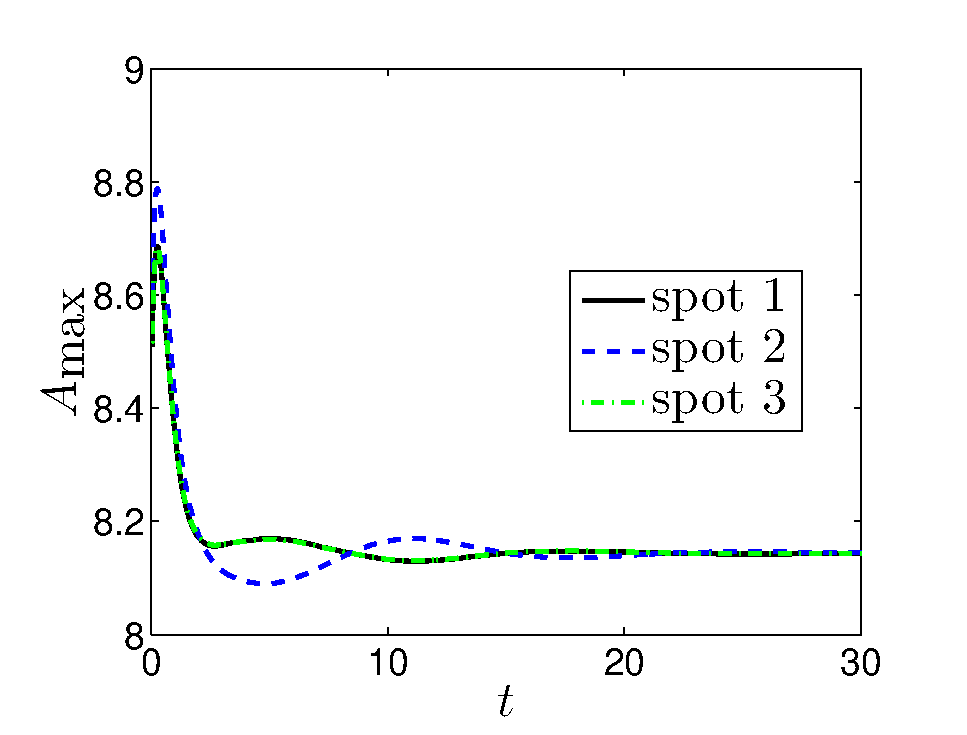
\includegraphics[width=0.32\textwidth,height=4.8cm]{figs/amp_3_run3.eps}
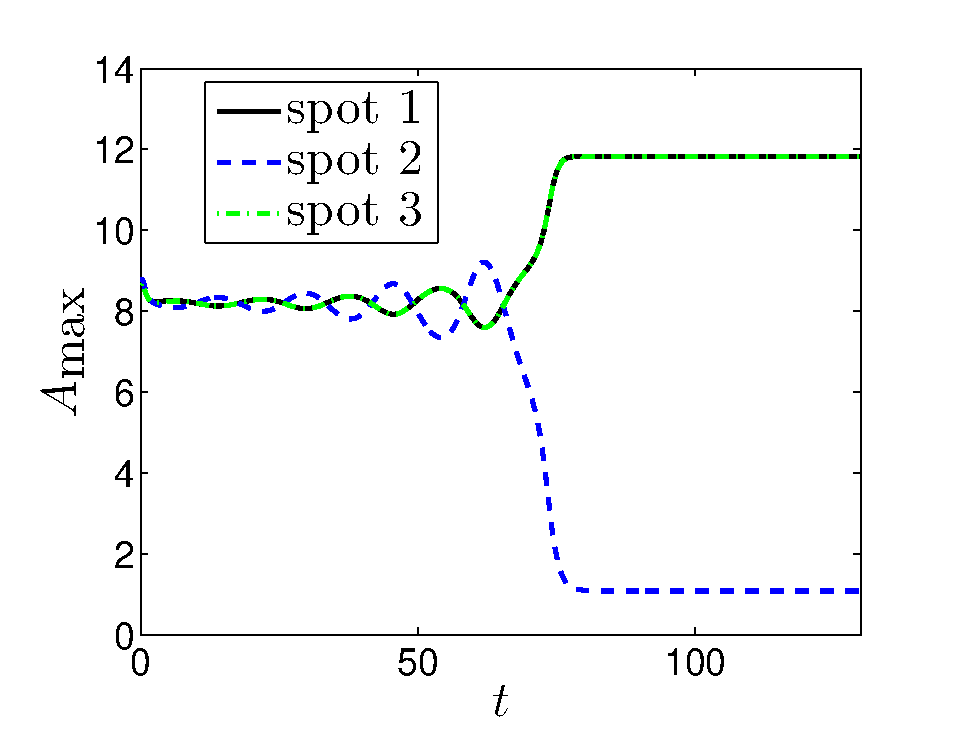
\includegraphics[width=0.32\textwidth,height=4.8cm]{figs/amp_3_run1.eps}
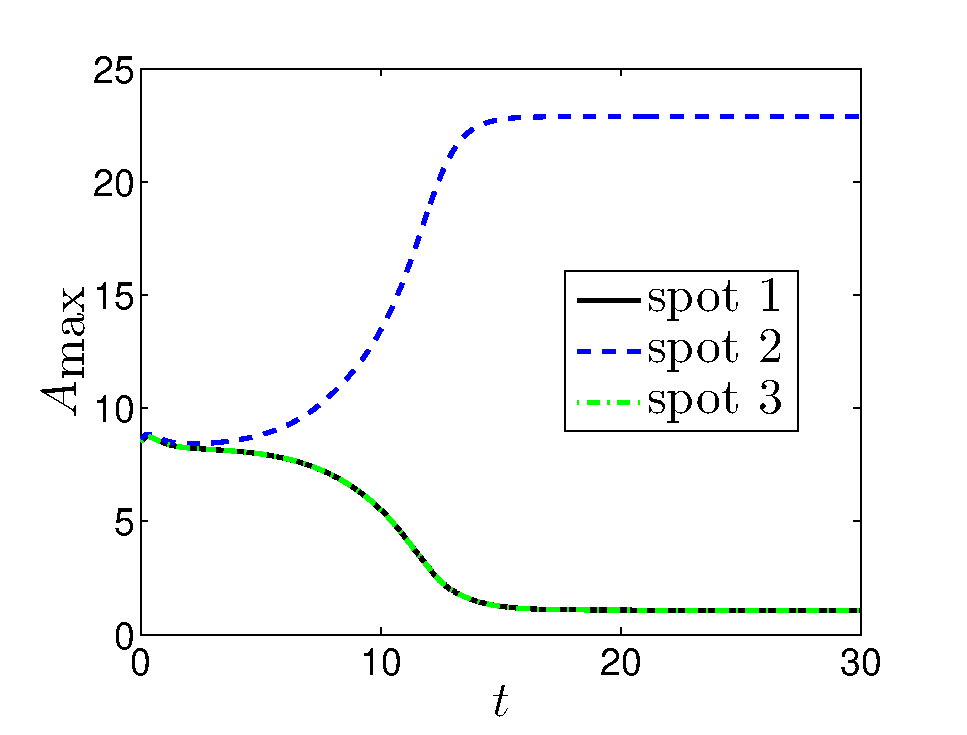
\includegraphics[width=0.32\textwidth,height=4.8cm]{figs/amp_3_run2.eps}
\caption{\label{fig:valid_3spot_q3} The spot amplitudes
  computed numerically from the full PDE system (\ref{eq:pol-main})
  for a three-spot pattern with $S=6$, $\gamma=2$, $\alpha=1$,
  $U_0=2$, $\epsilon=0.05$, and $q=3$.  Left panel: $\hat{\tau}_u=1.3$
  and ${\mathcal D}_0=0.07$, so that $\epsilon^2 D_p\approx
  0.0538$. Spot amplitudes are stable to asynchronous oscillations and
  to the competition instability.  Middle panel: $\hat{\tau}_u=2.5$
  and ${\mathcal D}_0=0.07$, so that $\epsilon^2 D_p=0.028$.  Spot
  amplitudes are unstable to asynchronous oscillations due to the
  sign-altering mode, which leads to the collapse of middle
  hotspot. Right panel: $\hat{\tau}_u=2.5$ and ${\mathcal D}_0=0.12$,
  so that $\epsilon^2 D_p=0.048$. Spot amplitudes are unstable to a
  competition instability due to the sign-altering mode, which leads
  to the collapse of the first and third hotspots. These results are
  consistent with the linear stability predictions in the left panels
  of Fig.~\ref{fig:hopf_tau_3} and Fig.~\ref{fig:hopf_pol_3}.  The
  results correspond to the marked points in the left panel of
  Fig.~\ref{fig:hopf_pol_3}. }
\end{figure}

\begin{figure}[htbp]
\centering
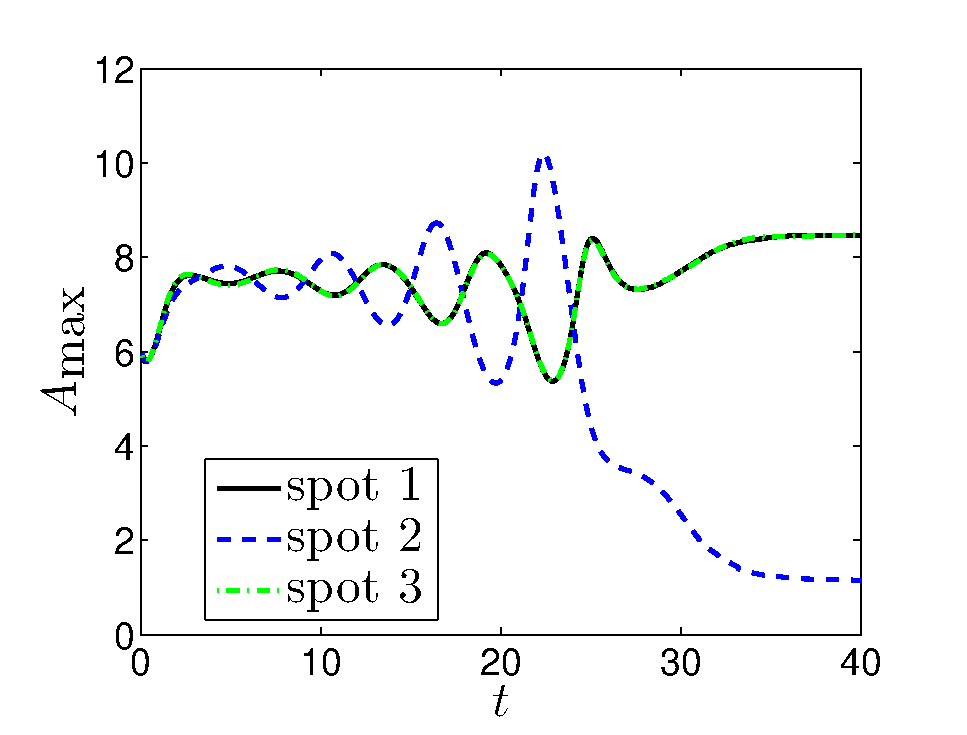
\includegraphics[width=0.47\textwidth,height=4.8cm]{figs/amp_3_run4.eps}
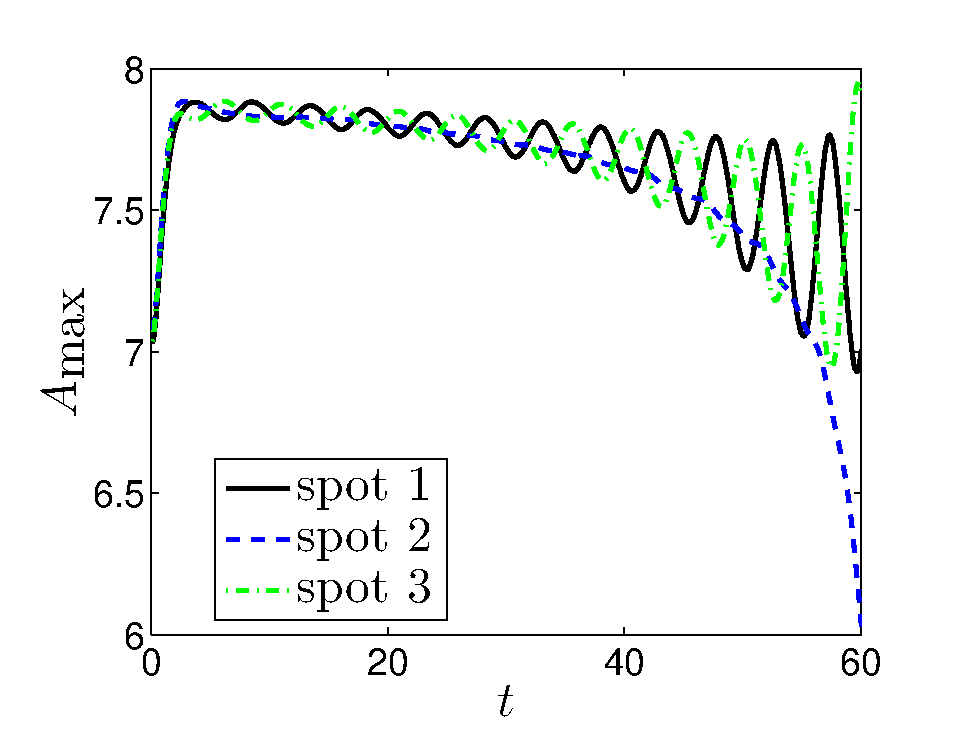
\includegraphics[width=0.47\textwidth,height=4.8cm]{figs/amp_3_run6.eps}
\caption{\label{fig:valid_3spot_q3_b} The spot amplitudes
  computed numerically from the full PDE system (\ref{eq:pol-main})
  for a three-spot pattern with $S=6$, $\gamma=2$, $\alpha=1$,
  $U_0=4$, $\epsilon=0.025$, and $q=3$, for the two marked points in the
  right panel of Fig.~\ref{fig:hopf_pol_3}. Left panel:
  $\hat{\tau}_u=2.5$ and ${\mathcal D}_0=0.01$, so that $\epsilon^2
  D_p\approx 0.004$. Unstable asynchronous spot amplitude oscillations
  are of sign-altering type as predicted by the theory. Right panel:
  $\hat{\tau}_u=1.6$ and ${\mathcal D}_0=0.03$, so that $\epsilon^2
  D_p=0.01875$.  The unstable spot amplitude oscillations are no
  longer sign-altering. Here the first and third spots exhibit
  anti-phase oscillations as predicted by the right panel of
  Fig.~\ref{fig:hopf_pol_3}.}
\end{figure}

As a more refined test of our linear stability theory, we again
consider a three-hotspot pattern but now take $U_0=4$ and
$\epsilon=0.025$. For $U_0=4$, the phase diagram shown in the right
panel of Fig.~\ref{fig:hopf_pol_3} predicts that there will be a
switch at some critical value of ${\mathcal D}_0$ between the dominant
spatial mode for asynchronous temporal oscillations. The full
numerical results for the spot amplitudes shown in
Fig.~\ref{fig:valid_3spot_q3_b} at the two marked points in the right
panel of Fig.~\ref{fig:hopf_pol_3} validate this theoretical
prediction. In particular, in the right panel of
Fig.~\ref{fig:valid_3spot_q3_b} we observe that it is the first and
third hotspots, instead of the first and second hotspots as in the
left panel of Fig.~\ref{fig:valid_3spot_q3_b}, that exhibit anti-phase
temporal oscillations.

\setcounter{equation}{0}
\setcounter{section}{5}
\section{Oscillatory Instabilities of the Hotspot Amplitudes: $q\protect\neq3$
and $q>1$}\label{sec:stab_qn3}

In this section we analyze the NLEP (\ref{stab:nlep_final_1}) for the
general case where $q\neq 3$, by determining the roots of
$\zeta(\lambda)=0$ in $\mbox{Re}(\lambda)>0$. In 
(\ref{stab:Cval_1}) we re-write ${\mathcal C}(\lambda)$ as
\begin{equation}\label{genq:C}
\mathcal{C}(\lambda)=\frac{\eta}{b}\left(1+\tilde{\tau}_{j}\lambda\right)
\left(1-\frac{b}{3-\lambda}\right)\,, \qquad\mbox{where} \qquad
\eta \equiv \frac{9\omega}{2qU_0}  \,, \quad 
b\equiv \frac{9\chi_{0,j}}{2}\,, \quad
\tilde{\tau}_{j} \equiv \frac{\hat{\tau}_{u}}{D_j \kappa_q} \,, \quad
 \frac{1}{\chi_{0,j}} = 1 + \frac{\kappa_3 D_j}{\alpha} \,.
\end{equation}
To relate our key parameter $b$ (which depends on $j$) to the
diffusivity ${\mathcal D}_0$, we first use the expression for
$\chi_{0,j}$ to write $D_j$ in terms of $b$ as
$D_{j}=\left[{\alpha/(2\kappa_3)}\right] \left({9/b}-2\right)$. Then,
upon using (\ref{q3:dlow}) for $\alpha/(2\kappa_3)$ and
(\ref{eq:pol-D_j}) to relate $D_j$ to ${\mathcal D}_0$, we obtain that
\begin{equation}\label{param:b}
      \frac{{\mathcal D}_0}{D^{-}_{0,j}}= \frac{9}{b}-2 \,, \qquad
  \mbox{or} \qquad   b = \frac{9}{2 + {\mathcal D}_0/D^{-}_{0,j}}  \,.
\end{equation}
Thus, ${\mathcal D}_0>0$ only when $b<{9/2}$.  Here $\dzjm$ is
defined in terms of the competition threshold ${\mathcal D}_{0c}$ of
(\ref{stab:zero_d0min}) by
\begin{equation}\label{param:dzjm}
   \dzjm \equiv \frac{{\mathcal D}_{0,c}}{\left(1+{q U_0/\omega}\right)}
  \left( \frac{1+\cos\left({\pi/K}\right)}
  {1-\cos\left({\pi j /K}\right)}\right) \,, \qquad
  \dzjp \equiv {\mathcal D}_{0,c} \left( \frac{1+\cos\left({\pi/K}\right)}
  {1-\cos\left({\pi j /K}\right)}\right) \,, \qquad
  \frac{\dzjp}{\dzjm}=1+ \frac{qU_0}{\omega} \,,
\end{equation}
where $D^{+}_{0,K-1}={\mathcal D}_{0,c}$.  In our analysis below, the
following ranges of $b$ will play a prominent role:
\bsub \label{genq:b_range}
\begin{align}
  (I):\quad  & 3<b<{9/2}  \quad \implies \quad \dzjm>{\mathcal D}_0>0 
   \quad \implies \quad {\mathcal C}(0)<0  \,, \\
  (II):\quad  & b_c\equiv {3\eta/\left(\eta + {3/2}\right)} < b< 3 \quad
    \implies \quad \dzjp >{\mathcal D}_0 >\dzjm \quad
    \implies \quad {1/2}>{\mathcal C}(0)>0 \,, \\
  (III):\quad  & b< b_c  \quad \implies \quad {\mathcal D}_0>\dzjp 
 \quad \implies \quad {\mathcal C}(0)>{1/2}\,.
\end{align}
\esub Since ${\mathcal F}(0)={1/2}$, and ${\mathcal C}(0)={1/2}$ when
$b=b_c$, we conclude that $b=b_c$ corresponds to a zero-eigenvalue
crossing.

\subsection{Analytical Results Based on the Winding Number Criterion}
\label{genq:wind_number}

Here we use the winding number criterion of \S \ref{sec:stab_arg} to
determine some rigorous results for the number $N$ of unstable
eigenvalues in $\mbox{Re}(\lambda)>0$ for the ranges of $b$ listed in
(\ref{genq:b_range}). In our analysis we will assume that Conjecture
\ref{conj:imag} on ${\mathcal F}_R(\lambda_I)$ and ${\mathcal
  F}_I(\lambda_I)$ holds for $q>1$.  With $\zeta(\lambda)$ as defined
in (\ref{stab:merom}), (\ref{key:wind}) when $\hat{\tau}_u>0$ yields
that
\begin{equation}\label{genq:wind}
  N = \frac{3}{2} + \frac{1}{\pi} \left[\arg \zeta \right]_{\Gamma_I^{+}} \,.
\end{equation}
To calculate $\left[\arg \zeta \right]_{\Gamma_I^{+}}$ we need the
following properties of the real and imaginary parts of ${\mathcal
  C}(i\lambda_I)$:

\begin{lem}\label{genq:prop_C} Let ${\mathcal C}(i\lambda_I)=
{\mathcal C}_R(\lambda_I) + i{\mathcal C}_{I}(\lambda_I)$. Then, from
(\ref{genq:C}) we have
\begin{equation}\label{genq:CrCI}
\mathcal{C}_{R}(\lambda_{I})  = \frac{\eta}{b}
 \left(1+\tilde{\tau}_{j} b-\frac{3b}{9+\lambda_{I}^{2}}
\left(1+3\tilde{\tau}_{j}\right)\right)\,, \qquad
\mathcal{C}_{I}(\lambda_{I})  =  \frac{\eta\lambda_{I}}{b}
  \left[ \tilde{\tau}_j - \frac{b(1+3\tilde{\tau}_j)}{(9+\lambda_{I}^{2})}
  \right]\,.
\end{equation}
For the imaginary part we have:
\begin{itemize}
\item [{(i)}] $\mathcal{C}_{I}(\lambda_{I})\sim \left(9 b\right)^{-1}
  \eta \lambda_{I}\left[3\tilde{\tau}_{j}(3-b)-b\right]$ as
  $\lambda_{I}\to 0^{+}$,
\item[{(ii)}] $\mathcal{C}_{I}(\lambda_{I})\sim b^{-1}\eta \tilde{\tau}_j
 \lambda_{I}$ as $\lambda_{I}\to+\infty$.
\item [{(iii)}] If $b<3/(1+\frac{1}{3\tilde{\tau}_{j}})$,
then $\mathcal{C}_{I}(\lambda_{I})>0$ for all $\lambda_I>0$.
\item[{(iv)}] If $b>3/(1+\frac{1}{3\tilde{\tau}_{j}})$, then
$\mathcal{C}_{I}(\lambda_{I})<0$ on $
0<\lambda_{I}<\sqrt{3(b-3)+\frac{b}{\tilde{\tau}_{j}}}\equiv\lambda_{I_{I}}$
and $\mathcal{C}_{I}(\lambda_{I})>0$ on $\lambda_I>\lambda_{I_{I}}$.
\end{itemize}
Alternatively, for the real part we have:
\begin{itemize}
\item [{(v)}] $\mathcal{C}_{R}^{\prime}(\lambda_{I})>0$ for $\lambda_{I}>0$.
\item [{(vi)}] ${\mathcal C}_{R}(\lambda_I)\sim
  b^{-1}\eta(1+\tilde{\tau}_j b)$ as $\lambda_I\to \infty$.
\item [{(vii)}] $\mathcal{C}_{R}(0)>0$ if $b<3$ and 
$\mathcal{C}_{R}(0)<0$ if $b>3$. When
$b>3$, then $\mathcal{C}_{R}(\lambda_{I})<0$ on 
$0<\lambda_{I}<\sqrt{\frac{3(b-3)}{1+\tilde{\tau}_{j}b}}\equiv \lambda_{IR}$,
and $\mathcal{C}_{R}(\lambda_{I})>0$ on $\lambda_I>\lambda_{IR}$.
\item [{(viii)}] $\mathcal{C}_{R}(0)>{1/2}$ iff $b<b_c\equiv
  {3\eta/(\eta+{3/2})}$, where $b_c$ is the zero-eigenvalue crossing.
\end{itemize}
\end{lem}

With properties (ii) and (vi) of Lemma \ref{genq:prop_C}, together
with the decay of ${\mathcal F}_R(\lambda_I)$ and ${\mathcal
  F}_I(\lambda_I)$ as $\lambda_I\to +\infty$ (see Proposition
\ref{rig:imag_f}), we conclude that
\begin{equation*}
\zeta(i\lambda_{I})\sim b^{-1}\eta \left(1+\tilde{\tau}_{j}b\right)+i
b^{-1}\eta \tilde{\tau}_{j}\lambda_{I} \quad \mbox{ as } \quad
\lambda_{I}\to+\infty\,.
\end{equation*}
Therefore, with respect to the origin, the path
$\zeta(i\lambda_I)=\zeta_R(\lambda_I)+i\zeta_I(\lambda_I)$ begins (as
$\lambda_I\to \infty$) asymptotically close to the positive infinity
of the imaginary axis in the complex $\zeta$ plane. 

Moreover, from property (v) of Lemma \ref{genq:prop_C}, and under 
Conjecture \ref{conj:imag} that ${\mathcal F}_R^{\prime}(\lambda_I)<0$
for all $\lambda_I>0$, we conclude that
\begin{equation}
\zeta_{R}^{\prime}(\lambda_{I})>0 \quad \mbox{for all} \quad
\lambda_{I}>0\,.\label{genq:zetar}
\end{equation}
With this key result, the path $\zeta(i\lambda_I)$ in the
$\zeta$-plane for $\lambda_I>0$ can only intersect the imaginary
$\zeta_I$ axis exactly one or zero times. In particular if
$\zeta(0)\equiv \zeta_R(0)>0$, then $\zeta_R(\lambda_I)>0$ for all
$\lambda_I>0$ so that $\left[\arg \zeta \right]_{\Gamma_I^{+}} =
-{\pi/2}$ and $N=1$ from (\ref{genq:wind}). In contrast, if
$\zeta(0)\equiv \zeta_R(0)<0$, then there is a unique
$\lambda_{I}^{\star}>0$ for which $\zeta_R(\lambda_I^{\star})=0$. In
this case, (\ref{genq:wind}) yields that
\bsub\label{genq:one_cross}
\begin{align}
   (I):\quad &  \zeta_I(\lambda_I^{\star})>0 \quad \implies  \quad
\left[\arg \zeta \right]_{\Gamma_I^{+}} = {\pi/2} \quad \implies \quad N=2\,
 \label{genq:N=2} \\
   (II):\quad &  \zeta_I(\lambda_I^{\star})<0 \quad \implies  \quad
\left[\arg \zeta \right]_{\Gamma_I^{+}} = {-3\pi/2} \quad \implies \quad N=0\,.
 \label{genq:N=0} 
\end{align}
\esub

With these preliminary observations, we obtain the following
instability result for the $j$-th mode on the range ${\mathcal D}_0>\dzjp$.

\begin{prop}\label{prop:genq:N=1} Suppose that ${\mathcal D}_0>\dzjp$ and 
that Conjecture \ref{conj:imag} holds. Then, for the $j$-th mode with
$j=1,\ldots,K-1$, we have $N=1$ for all $\tilde{\tau}_j\geq 0$.
\end{prop}

\begin{proof} When ${\mathcal D}_0>\dzjp$, we have 
$b<b_c\equiv {3\eta/(\eta+{3/2})}$ and consequently ${\mathcal
    C}_R(0)>{1/2}$ from (III) of (\ref{genq:b_range}). This yields
  $\zeta_R(0)>0$, and thus $\zeta_R(\lambda_I)>0$ for all
  $\lambda_I>0$ using the monotonicity result (\ref{genq:zetar}),
  which holds when ${\mathcal F}_R^{\prime}(\lambda_I)<0$ for all
  $\lambda_I>0$. Therefore $\left[\arg \zeta \right]_{\Gamma_I^{+}}
  =-{\pi/2}$ and (\ref{genq:wind}) yields $N=1$ for all
  $\tilde{\tau}_j>0$.
\end{proof}

Together with the ordering principle $D^{+}_{0,j+1}<D^{+}_{0,j}$ for
$j=1,\ldots, K-2$ from (\ref{q3:d_order}), this instability result
proves, for any $\hat{\tau}_u>0$, that there are exactly $K-1$
positive real eigenvalues of the NLEP (\ref{stab:nlep_final_1}) when
${\mathcal D}_0>D^{+}_{0,1}$.

\begin{prop}\label{prop:genq:N=02} Suppose that ${\mathcal D}_0<\dzjp$ and 
that Conjecture \ref{conj:imag} holds. Then, for the $j$-th mode with
$j=1,\ldots,K-1$, we have either $N=0$ or $N=2$ for all $\tilde{\tau}_j>0$.
Moreover, if $\tilde{\tau}_j\ll 1$ we have $N=0$.
\end{prop}

\begin{proof}
If ${\mathcal D}_0<\dzjp$, then $b>{3\eta/(\eta+{3/2})}$, and so
${\mathcal C}_R(0)<{1/2}$ by (II) of (\ref{genq:b_range}). Therefore,
since $\zeta_{R}(0)<0$, $\zeta_R(\infty)>0$, and
$\zeta_R^{\prime}(\lambda_I)>0$, which holds when ${\mathcal
  F}_R^{\prime}(\lambda_I)<0$ for all $\lambda_I>0$, it follows that
there is a unique root $\lambda_I^{\star}$ for which
$\zeta_R(\lambda^{\star}_I)=0$. From (\ref{genq:one_cross}), we have
for all $\hat{\tau}_j>0$ that either $N=0$ or $N=2$ depending on the sign of
$\zeta_I(\lambda_I^{\star})$. 

Next, we prove that $N=0$ if $\tilde{\tau}_j\ll 1$. For
$\tilde{\tau}_j\ll 1$, (\ref{genq:CrCI}) yields that
\begin{equation*}
    {\mathcal C}_R(\lambda_I) \sim \frac{\eta}{b}\left( 1 - 
 \frac{3b}{9+\lambda_I^2} \right) \,,
\end{equation*}
uniformly in $\lambda_I$. It follows that
$\zeta_R(\lambda_I^{\star})=0$ at some $\lambda_I^{\star}={\mathcal
  O}(1)$ when $\tilde{\tau}_j\ll 1$.  However, for $\tilde{\tau}_j\ll
1$, we have from (\ref{genq:CrCI}) that ${\mathcal
  C}_I(\lambda_I^{\star})\sim -{\eta
  \lambda_I/\left(9+\lambda_I^2\right)}<0$.  Under Conjecture
\ref{conj:imag} that ${\mathcal F}_I(\lambda_I)>0$, we conclude that
$\zeta_I(\lambda_I^{\star})={\mathcal C}_{I}(\lambda_I^{\star})-
    {\mathcal F}_{I}(\lambda_{I}^{\star})<0$. Therefore, from
    (\ref{genq:N=0}) we conclude that $N=0$.
\end{proof}

This result proves that the $j$-th mode is linearly stable on the
range ${\mathcal D}_0<\dzjp$ whenever $\tilde{\tau}_j\ll 1$. The next
result determines $N$ for $\tilde{\tau}_j\gg 1$ on the entire range
${\mathcal D}_0<\dzjp$.

\begin{prop}\label{prop:genq:hopf} Suppose that $\dzjm<{\mathcal D}_0<\dzjp$
and that Conjecture \ref{conj:imag} holds. Then, for the $j$-th mode
with $j=1,\ldots,K-1$, we have $N=2$ when $\tilde{\tau}_j \gg 1$.  In
contrast, if ${\mathcal D}_0<\dzjm$, then $N=0$ when $\tilde{\tau}_j
\gg 1$.
\end{prop}

\begin{proof}
We first observe from (\ref{genq:b_range}) that $\dzjm<{\mathcal
  D}_0<\dzjp$ when $b_c<b<3$ and ${\mathcal D}_0<\dzjm$ when
$b>3$. For ${\mathcal D}_0<\dzjp$, we have $\zeta_R(0)<0$ and so there
is a unique root $\lambda_I^{\star}$ to
$\zeta_R(\lambda_I^{\star})=0$. For $\tilde{\tau}_j\gg 1$, and for
$b>b_c\equiv {3\eta/(\eta+{3/2})}$, this unique root of
$\zeta_R(\lambda_I)$ occurs for $\lambda_I={\mathcal
  O}(\tilde{\tau}_j^{-1/2})\ll 1$. By setting ${\mathcal
  C}_R(\lambda_I)={\mathcal F}_{R}(\lambda_I)$, and using
$\lambda_I={\mathcal O}(\tilde{\tau}_j^{-1/2})\ll 1$ together with
(\ref{genq:CrCI}) for ${\mathcal C}_R$, we get that
\begin{equation*}
  \frac{\eta}{b} \left( 1 + \frac{b}{9} (\tilde{\tau}_j \lambda_I^2-3)
  \right) \sim {\mathcal F}_R(0)=\frac{1}{2} \,.
\end{equation*}
In this way, we obtain for $\tilde{\tau}_j\gg 1$ that the unique root
$\lambda_{I}^{\star}$ of $\zeta_R(\lambda_I)=0$ occurs when
\begin{equation}
   \lambda_{I}^{\star} \sim {\beta/\tilde{\tau}_j^{1/2}} \,, \qquad 
 \beta \equiv \sqrt{3 \left(1- \frac{3}{b}\right) + \frac{9}{2\eta}}\,.
\end{equation}
From (\ref{genq:CrCI}) for ${\mathcal C}_I$, we then calculate for
$\tilde{\tau}_j\gg 1$ that
\begin{equation}\label{shit:eq}
   {\mathcal C}_I(\lambda_I^{\star}) \sim \frac{\eta\beta}{3b}(3-b) 
  \tilde{\tau}_j^{1/2} = {\mathcal O}(\tilde{\tau}_j^{1/2}) \,.
\end{equation}
When $b>3$, corresponding to ${\mathcal D}_0<\dzjm$, we have ${\mathcal
  C}_I(\lambda_I^{\star})<0$. Therefore, with ${\mathcal
  F}_I(\lambda_I)>0$ from Conjecture \ref{conj:imag}, we conclude that
$\zeta_I(\lambda_{I}^{\star})<0$. This yields that $N=0$ from
(\ref{genq:N=0}). Now suppose that $b_c<b<3$, corresponding to
$\dzjm<{\mathcal D}_0<\dzjp$.  Then, since ${\mathcal
  C}_I(\lambda_I^{\star})>0$, with ${\mathcal
  C}_I(\lambda_I^{\star})=\tilde{\tau}_j^{1/2}\gg 1$ for
$\tilde{\tau}_j\gg 1$, while ${\mathcal
  F}_I(\lambda_I^{\star})={\mathcal O}(1)$, we conclude that
$\zeta_I(\lambda_I^{\star})>0$. This yields that $N=2$ from 
(\ref{genq:N=2}).
\end{proof}

On the range $\dzjm<{\mathcal D}_0<\dzjp$, Propositions
\ref{prop:genq:hopf} and \ref{prop:genq:N=02} show for the $j$-th mode
that $N=2$ for $\tilde{\tau}_j\gg 1$ and $N=0$ for $\tilde{\tau}_j\ll
1 $. Therefore, by continuity, there is a Hopf bifurcation value of
$\tilde{\tau}_j$ on this range of ${\mathcal D}_0$. Although this
proves the existence of a Hopf bifurcation threshold for
$\hat{\tau}_u$ on the range $\dzjm<{\mathcal D}_0<\dzjp$ for any mode
$j=1,\ldots,K-1$, it does not establish uniqueness of this threshold 
or provide any its qualitative properties. This is done numerically in
\S \ref{genq:param}.

The remaining issue relates to the range ${\mathcal D}_0<\dzjm$, where
we have proved that $N=0$ when either $\tilde{\tau}_j\ll 1$ or
$\tilde{\tau}_j\gg 1$. Next, we study for this range of ${\mathcal
  D}_0$ whether $N=0$ {\em for all} $\tilde{\tau}_j>0$.

To examine this question we will proceed as follows: Suppose that
${\mathcal C}_R(0)<{1/2}$ and that ${\mathcal C}_{R}(\infty)>{1/2}$.
Then, with Conjecture \ref{conj:imag} that ${\mathcal
  F}_R^{\prime}(\lambda_I)<0$ for all $\lambda_I>0$, and with
${\mathcal F}_R(0)={1/2}$, it follows that the unique root
$\lambda_{I}^{\star}$ to $\zeta_R(\lambda_I)=0$ satisfies
$\lambda_{I}^{\star}<\lambda_{Im}$ where $\lambda_{Im}$ is defined by
$C_{R}(\lambda_{Im})={1/2}$. If we can then show that
$C_{I}(\lambda_{Im})<0$, it follows that
$C_{I}(\lambda_{I}^{\star})<0$. Then, by Conjecture \ref{conj:imag}
that ${\mathcal F}_I(\lambda_I)>0$ for all $\lambda_I>0$, we obtain
that $\zeta_I(\lambda_{I}^{\star})<0$, and consequently $N=0$ from
(\ref{genq:N=0}).  Therefore, our goal is to determine the range of
$b$, with $b>3$, for which
\begin{equation}\label{genq:bound}
      {\mathcal C}_{R}(0)<{1/2} \,, \qquad
{\mathcal C}_{R}(\infty)>{1/2} \,, \qquad \mbox{and} \quad
  {\mathcal C}_{I}(\lambda_{Im})<0  \quad \mbox{where} \quad
 {\mathcal C}_{R}(\lambda_{Im}) = {1/2} \,.
\end{equation}

When $b>b_c$ we have ${\mathcal C}_R(0)<1/2$, and from property (vi)
of Lemma \ref{genq:prop_C} we have ${\mathcal C}_R(\infty)>{1/2}$
provided that
\begin{equation}\label{eq1:gap}
   \frac{\eta}{b} \left(1+ \tilde{\tau}_j b\right) > \frac{1}{2}\,.
\end{equation}
Now by using (\ref{genq:CrCI}) for ${\mathcal C}_R$, we obtain that
${\mathcal C}_R(\lambda_{Im})={1/2}$ when
\begin{equation*}
     \frac{1+3\tilde{\tau}_j}{9+\lambda_{Im}^2} = \frac{1}{3\eta} \left[
   \frac{\eta}{b} (1+\tilde{\tau}_j b) - \frac{1}{2}\right]\,.
\end{equation*}
By using this expression in (\ref{genq:CrCI}) for ${\mathcal
  C}_I(\lambda_I)$ we get, after some algebra, that
\begin{equation*}
    {\mathcal C_{I}}(\lambda_{Im}) = \frac{\eta \lambda_{Im}}{b} \left(
  \tilde{\tau}_j - \frac{b (1+3\tilde{\tau}_j)}{9+\lambda_{Im}^2} \right)
  = -\frac{\eta \lambda_{Im}}{3b} \left[ \tilde{\tau}_j (b-3) + 1 - 
  \frac{b}{2\eta} \right] \,.
\end{equation*}
We conclude that ${\mathcal C_{I}}(\lambda_{Im})<0$ when
$1+\tilde{\tau}_j b - {b/(2\eta)}>3\tilde{\tau}_j$. 
Since, from (\ref{eq1:gap}),  we have ${\mathcal C}_R(\infty)>{1/2}$ when
$1+\tilde{\tau}_j b - {b/(2\eta)}>0$, we conclude that the inequalities in 
(\ref{genq:bound}) hold when
\begin{equation}\label{eq2:gap}
   b>b_c \equiv \frac{3\eta}{\eta + {3/2}} \qquad \mbox{and} \qquad
1+\tilde{\tau}_j b - {b/(2\eta)}>3 \tilde{\tau}_j \,.
\end{equation}

We now determine a range of $b$, independent of $\tilde{\tau}_j$, for
which the inequalities (\ref{eq2:gap}) hold.  A sufficient condition
for (\ref{eq2:gap}) to hold is that $b>3$ and $b<2\eta$. If
$\eta<{3/2}$, there is no such range of $b$. If $\eta>{9/2}$, 
these inequalities hold on the full range $3<b<{9/2}$ where ${\mathcal
  D}_0<\dzjm$, as given in (I) in (\ref{genq:b_range}). However, when
${3/2}<\eta<{9/2}$, the interval $3<b<2\eta$ is only a subset of the
full range in (I) of (\ref{genq:b_range}) where ${\mathcal
  D}_0<\dzjm$.  By using (\ref{genq:C}) for $\eta$, together with
(\ref{param:b}) to relate $b$ to ${\mathcal D}_0$, we summarize our
result as follows:

\begin{prop}\label{prop:genq:gap} Suppose that Conjecture \ref{conj:imag} 
holds. Then, for the $j$-th mode with $j=1,\ldots,K-1$ we have the following:
\bsub\label{genq:gap}
\begin{align}
  (I) \quad  &\mbox{Suppose } U_0<{2\omega/q} \mbox{ and } 
    {\mathcal D}_0<\dzjm\,. \mbox{ Then } N=0 \,\, \mbox{for all }
     \hat{\tau}_u >0 \,.\label{genq:gap_1} \\
  (II) \quad  &\mbox{Suppose } {2\omega/q} < U_0<{3\omega/q} \mbox{ and } 
    \left(\frac{q U_0}{\omega}-2\right) \dzjm<{\mathcal D}_0<\dzjm\,. 
   \mbox{ Then } N=0 \,\, \mbox{for all } \hat{\tau}_u>0 \,.\label{genq:gap_2}
\end{align}
\esub This result provides no stability information for the range
${\mathcal D}_0<\dzjm$ when $U_0>{3\omega/q}$. 
\end{prop}

As a result of the ordering principle $D^{-}_{0,K-1}<D^{-}_{0,j}$ for
$j=1,\ldots,K-2$ and $K\geq 3$, we conclude from (I) of Proposition
\ref{prop:genq:gap}, upon recalling $\omega=S(\gamma-\alpha)-U_0$,
that a $K$-hotspot pattern is linearly stable for all $\hat{\tau}_u>0$
on the range ${\mathcal D}_0<D^{-}_{0,K-1}$ when
$U_0<{2S(\gamma-\alpha)/(q+2)}$. This result is weaker than that
obtained for the explicitly solvable case $q=3$, In fact, since
$\omega=S(\gamma-\alpha)-U_0$, it provides no stability information on
${\mathcal D}_0<D^{-}_{0,j}$ when $U_0>3{(S-\gamma)/(q+3)}$. For
$q=3$, we recall from Proposition \ref{q3:roots_quad} that for the
$j$-th mode we have $N=0$ for ${\mathcal D}_0<\dzjm$ for all
$\hat{\tau}_u>0$ without any restriction on $U_0$.

In \S \ref{genq:param} we will investigate numerically the possibility
of a Hopf bifurcation for the range $0<{\mathcal D}_0<D^{-}_{0,j}$
when $U_0>{3\omega/q}$, for which Proposition \ref{prop:genq:gap} does not
apply. Our numerical procedure in \S \ref{genq:param} suggests that
no Hopf bifurcation exists on the range $0<{\mathcal
  D}_0<D^{-}_{0,j}$ for any $U_0<U_{0,\max}$, as qualitatively identical to
the second statement proved in Proposition \ref{q3:roots_quad} for the
explicitly solvable case $q=3$.

To gain some insight into the behavior of the Hopf bifurcation
threshold $\tilde{\tau}_{j}$ for the $j$-th mode, we now derive a
scaling law for it to show that $\tilde{\tau}_{j}\to
\infty$ and $\lambda_{I}\to 0^{+}$ as ${\mathcal D}_0\to D^{-}_{0,j}$
from above, or equivalently as $b\to 3$ from below.  For $b\to 3^{-}$,
we look for a solution to $\zeta(i\lambda_I)=0$ with $\lambda_I\to
0$, $\tilde{\tau}_j\to \infty$, with the distinguished balance
$\lambda_{I}={\mathcal O}(\tilde{\tau}_j^{-1/2})$.  By setting
${\mathcal C}_R(\lambda_I)={\mathcal F}_{R}(\lambda_I)$, and using
${\mathcal F}_{R}(\lambda_I)\sim {1/2}$ together with (\ref{genq:CrCI}) for
${\mathcal C}_R$, we get that
\begin{equation*}
    \frac{\eta}{b} \left(1 - \frac{b}{9} \left(3 - \tilde{\tau}_j \lambda_I^2
  \right)\right) \sim \frac{1}{2} \,.
\end{equation*}
By solving for $\tilde{\tau}_j\lambda_I^2$ and letting $b\to 3$, we obtain 
that $\tilde{\tau}_j\lambda_I^2 = 9/(2\eta) + {3(b-3)/b}$. By letting $b\to 3$,
we conclude that
\begin{equation}\label{genq:lami_asy}
    \lambda_I \sim \sqrt{ \frac{9}{2\eta\tilde{\tau}_j}}  
 \,, \qquad \mbox{as} \quad \tilde{\tau}_j \to \infty \,.
\end{equation}
Then, we set ${\mathcal C}_I(\lambda_I)={\mathcal F}_I(\lambda_I)$, and use
(\ref{genq:CrCI}) for ${\mathcal C}_I$, together with the local behavior 
for ${\mathcal F}_I(\lambda_I)$ as $\lambda_I\to 0$ from (iv) of 
Proposition \ref{rig:imag_f}. This yields that
\begin{equation*}
    \frac{\eta\lambda_I}{b(9+\lambda_I^2)} \left(3 \tilde{\tau}_j(3-b)-b
  + \tilde{\tau}_j \lambda_I^2\right) \sim \frac{\lambda_I}{4}\left(1 -
  \frac{1}{q}\right) \,.
\end{equation*}
Upon cancelling the factor of $\lambda_I$ and using 
$\tilde{\tau}_j\lambda_I^2\sim {9/(2\eta)}$, we solve for $\tilde{\tau}_j$
in the expression above to get
\begin{equation}\label{genq:shit_m}
   \tilde{\tau}_j \sim \frac{1}{3(3-b)} \left[ b - \frac{9}{2\eta} +
  \frac{9b}{4\eta}\left(1 - \frac{1}{q}\right) \right] \sim
 \frac{1}{3-b} \left[1 + \frac{3}{4\eta}
   \left(1- \frac{3}{q}\right) \right] \,, \quad \mbox{as} \quad b \to 3\,.
\end{equation}
In terms of the original variables ${\mathcal D}_0$, $U_0$ and
$\hat{\tau}_u$ we use (\ref{genq:C}) and (\ref{param:b}) to get
\begin{equation}\label{genq:form}
   \frac{3}{4\eta}=\frac{qU_0}{6\omega} \,, \qquad 
  \hat{\tau}_u = \frac{\alpha}{2} \left( \frac{\kappa_q}{\kappa_3}\right)
   \frac{{\mathcal D}_0}{D^{-}_{0,j}}  \tilde{\tau}_j \,, \qquad
   b-3 \sim 1- \frac{{\mathcal D}_0}{{\mathcal D}^{-}_{0,j}} 
  \quad \mbox{as} \quad  {\mathcal D}_0\to D^{-}_{0,j} \,.
\end{equation}
Upon substituting (\ref{genq:form}) into (\ref{genq:shit_m}) and
(\ref{genq:lami_asy}) we get the limiting Hopf bifurcation threshold
\begin{equation}\label{genq:asy_bto3}
  \hat{\tau}_{u,H}\sim \frac{\alpha}{2} \left( \frac{\kappa_q}{\kappa_3}\right)
   \frac{1}{\left({{\mathcal D}_0/D^{-}_{0.j}} -1\right)} 
 \left( 1 + \frac{qU_0}{6\omega} \left(1 - \frac{3}{q}\right) \right)^{1/2} \,,
 \qquad
  \lambda_{IH}\sim \sqrt{ \frac{{\mathcal D}_0}{D^{-}_{0,j}}-1 }
   \left( \frac{qU_0}{\omega} \right)^{1/2} 
   \left[ 1 + \frac{qU_0}{6\omega}
   \left(1 - \frac{3}{q}\right) \right]^{-1/2} \,,
\end{equation}
as ${\mathcal D}_0\to D^{-}_{0,j}$.  For the special case where $q=3$,
this limiting result for $\lambda_{IH}$ and $\hat{\tau}_{u,H}$ agrees with
that in (\ref{q3:lim_val}) and (\ref{q3:tau_lim}), respectively.

Finally, for the $j$-th mode we will calculate an additional scaling
law for the Hopf bifurcation threshold and the Hopf eigenvalue as
$b\to b_c\equiv {3\eta/(\eta+{3/2})}$ from above, corresponding to the
limit ${\mathcal D}_0\to D^{+}_{0,j}$ from below. We look for a root
$\lambda_I\ll 1$ to ${\mathcal C}_R(\lambda_I)={\mathcal
  F}_R(\lambda_I)$ and use
\begin{equation}\label{genq:kr}
    {\mathcal F}_{R}\sim \frac{1}{2} - k_R \lambda_I^2 + \cdots \,, \quad
\mbox{as} \quad \lambda_I \to 0 \,,
\end{equation}
for some $k_R>0$, together with (\ref{genq:CrCI}) for ${\mathcal
  C}_R(\lambda_I)$, to obtain that
\begin{equation*}
     \frac{\eta}{b(9+\lambda_I^2)} \left[ 9 -3b + \lambda_I^2
   (1+\tilde{\tau}_j b) \right] \sim \frac{1}{2} - k_R \lambda_I^2 \,.
\end{equation*}
Upon isolating $\lambda_I$, we get
\begin{equation}\label{genq:zero}
     \frac{\eta}{b}(9-3b) - \frac{9}{2} = \lambda_I^2 \left( \frac{1}{2}
   - 9\kappa_R - \frac{\eta}{b_c} \left(1+\tilde{\tau}_j b_c\right)\right)\,.
\end{equation}
We then set ${\mathcal C}_I(\lambda_I)={\mathcal F}_I(\lambda_I)$ as 
$\lambda_I\to 0$ using the local behavior (i) of Lemma
\ref{genq:prop_C} for ${\mathcal C}_I(\lambda_I)$ and that in
(iv) of Proposition \ref{rig:imag_f} for ${\mathcal F}_{I}(\lambda_I)$.
This yields that
\begin{equation*}
   \frac{\eta}{9b_c} \left( 3\tilde{\tau}_j (3-b_c) - b_c\right) \sim
  \frac{1}{4}\left( 1 - \frac{1}{q}\right) \,.
\end{equation*}
Upon using $b_c={3\eta/(\eta+{3/2})}$, we solve for $\tilde{\tau}_j$
in this expression to obtain
\begin{equation}\label{genq:z1}
   \tilde{\tau}_j \sim \frac{2\eta}{9} \left[ 1 + \frac{9}{4\eta}
  \left( 1 - \frac{1}{q} \right) \right]\,, \quad \mbox{as} \quad 
b \to b_c \,.
\end{equation}
Upon substituting (\ref{genq:z1}) into (\ref{genq:zero}) and solving
for $\lambda_I$ we obtain, after some algebra, that $\lambda_I\equiv
\lambda_{IH}$ satisfies
\begin{equation}\label{genq:z1_lam}
\lambda_{IH} \sim \sqrt{\frac{27}{2}} \left( \frac{1-{b_c/b}}{3-b_c}\right)^{1/2}
  \left( 9\kappa_R + \frac{\eta}{3} + \frac{2\eta^2}{9} + \frac{\eta}{2}
  \left(1- \frac{1}{q}\right) \right)^{-1/2} \,, \quad \mbox{as} \quad
 b \to b_c \,.
\end{equation}
To write $\tilde{\tau}_j$ in (\ref{genq:z1}) in terms of the original
variables, we use (\ref{genq:form}), together with
${D^{+}_{0,j}/D^{-}_{0,j}}=1+{qU_0/\omega}$, to obtain
\begin{equation}\label{genq:final_lim}
   \hat{\tau}_{u,H}\sim \frac{\alpha\omega}{2q U_0} 
  \left( \frac{\kappa_q}{\kappa_3} \right) \left( 1 + \frac{q U_0}{\omega} 
 \right) \left( 1 + \frac{U_0}{2\omega}(q-1)\right) \,, \qquad
 \mbox{as} \quad {\mathcal D}_0 \to D^{+}_{0,j} \,.
\end{equation}

When $q=3$, the expression in (\ref{genq:final_lim}) agrees with that
obtained in (\ref{q3:tau_lim}) for the explicitly solvable case.  To
determine if (\ref{genq:z1_lam}) yields the limiting Hopf eigenvalue
given in (\ref{q3:lim_val}) when $q=3$, we use ${\mathcal
  F}(i\lambda_I)={3/\left[2(3-i\lambda_I)\right]}$, from
(\ref{eq:exactF_q3}). This yields ${\mathcal F}_R(\lambda_I)\sim
{1/2}-{\lambda_I^2/18}$, which identifies $k_R={1/18}$ in
(\ref{genq:kr}). With this value for $k_R$ and $q=3$, the expression
in the brackets in (\ref{genq:z1_lam}) is a perfect square, and
simplifies to
\begin{equation*}
\lambda_{IH} \sim \sqrt{\frac{27}{2}} \left( 1-\frac{b_c}{b} \right)^{1/2}
 \frac{\left(9/2\right)^{1/2}}{(3-b_c)^{1/2} (\eta+{3/2})} \,.
\end{equation*}
We then use $b_c={3\eta/(\eta+{3/2})}$ together with
$\eta={3\omega/(2U_0)}$ when $q=3$ from (\ref{genq:C}), to get
\begin{equation}\label{genq:up_lim}
\lambda_{IH} \sim \sqrt{\frac{27}{2}} \sqrt{ 1-\frac{b_c}{b}} 
 \left( 1 + \frac{\omega}{U_0}\right)^{-1/2} \,.
\end{equation}
Finally, we use (\ref{param:b}) for $b$,
${D^{+}_{0,j}/D^{-}_{0,j}}=1+3{U_0/\omega}$, and
$\eta={3\omega/(2U_0)}$ to calculate
\begin{equation}
  \frac{b_c}{b}-1 = \frac{\eta}{3(\eta+{3/2})}\left( \frac{{\mathcal D}_0}
   {{\mathcal D}^{-}_{0,j}}+2\right) = \left(\frac{{\mathcal D}_0} {
   D^{+}_{0,j}} -1\right) \left(\frac{ {1+3U_0/\omega}}{3\left(1+ 
{U_0/\omega}\right)}\right) \,.
\end{equation}
Upon substituting this expression into (\ref{genq:up_lim}), we recover
the result for $\lambda_{IH}$ given in (\ref{q3:lim_val}) for
${\mathcal D}_0\to D^{+}_{0,j}$ from below.

\subsection{Parameterization of the Hopf Bifurcation Curve}\label{genq:param}

To compute the Hopf bifurcation threshold numerically for the $j$-th
mode on the range $\dzjm<{\mathcal D}_0<\dzjp$, and to explore the
range ${\mathcal D}_0<\dzjm$ where Proposition \ref{prop:genq:gap} only gives
partial stability information, we now formulate a convenient
parameterization of any Hopf bifurcation curve in the $\hat{\tau}_u$
versus ${\mathcal D}_0$ parameter plane.

We set $\zeta(i\lambda_I)=0$ in (\ref{stab:merom}) to get ${\mathcal
  C}(i\lambda_I)={\mathcal F}(i\lambda_I)$, where ${\mathcal
  C}(i\lambda_I)$ and ${\mathcal F}(i\lambda_I)$ are given in
(\ref{genq:C}) and (\ref{eq:pol-F_R-F_I}) respectively. By taking the
squared modulus of both sides we get
\begin{equation*}
   \frac{\eta^2}{b^2} \left( 1 + \tilde{\tau}_j^2 \lambda_I^2\right)
 \left[ \frac{ (3-b)^2 + \lambda_I^2}{9+\lambda_I^2}\right] = 
  | {\mathcal F}(i\lambda_I)|^{2} \,,
\end{equation*}
which we solve for $\tilde{\tau}_j^2$ to get
\begin{equation}\label{param:mod}
  \tilde{\tau}_j^2 = \frac{1}{\lambda_I^2} \left[ -1 + \frac{b^2}{\eta^2}
     \left( \frac{9+\lambda_I^2}{(3-b)^2+\lambda_I^2} \right) 
  | {\mathcal F}(i\lambda_I)|^{2} \right] \,.
\end{equation}
To derive a second equation for $\tilde{\tau}_j$ we set 
$\mbox{Im}\left[\zeta(i\lambda_I)\right]=0$ to get, upon using 
(\ref{genq:CrCI}) for ${\mathcal C}_I(\lambda_I)$, that
\begin{equation*}
\frac{\eta\lambda_{I}}{b(9+\lambda_{I}^{2})}
\left(3\tilde{\tau}_{j}\left(3-b\right)-b+\tilde{\tau}_{j}\lambda_{I}^{2}\right)
 = {\mathcal F}_{I}(\lambda_I) \,.
\end{equation*}
Upon isolating $\tilde{\tau}_j$ from this expression we obtain that
\begin{equation}\label{param:tau}
   \tilde{\tau}_j = \frac{b}{\eta \lambda_I} \frac{
\left[\eta \lambda_I + \mu {\mathcal F}_{I}(\lambda_I)\right]}{\mu - 3b}
 \,, \qquad \mbox{where} \quad \mu \equiv 9+\lambda_I^2 \,.
\end{equation}
Then, by eliminating $\tilde{\tau}_j$ between (\ref{param:mod}) and
(\ref{param:tau}) we obtain, after some algebra, that $\lambda_I$ must
satisfy the nonlinear algebraic problem ${\mathcal M}(\lambda_I)=0$,
defined by 
\bsub \label{param:all}
\begin{equation}\label{param:nroot}
   {\mathcal M}(\lambda_I)\equiv  (\mu+b^2-6b)\left[
 \left(\eta \lambda_I + \mu {\mathcal F}_I \right)^2 + 
  \frac{\eta^2}{b^2}(\mu-3b)^2 \right]  - \mu (\mu-3b)^2
 |{\mathcal F}|^2  \,,  \qquad \mbox{where} \quad
  \mu\equiv 9 + \lambda_I^2 \,.
\end{equation}
Here we have labeled ${\mathcal F}_I\equiv {\mathcal F}_I(\lambda_I)$
and $|{\mathcal F}|^2 \equiv |{\mathcal F}(i\lambda_I)|^2 =\left[{\mathcal
  F}_R(\lambda_I)\right]^2 + \left[{\mathcal F}_I^{2}(\lambda_I)\right]^2$.
In terms of the original $\hat{\tau}_u$ variable, we have from
(\ref{genq:form}) and ${\mathcal D}_0/D^{-}_{0,j}={9/b}-2$ that the
Hopf bifurcation threshold is
\begin{equation}\label{param:new_tau}
   \hat{\tau}_{u,H} = \frac{\alpha}{2\eta\lambda_I} \left(\frac{\kappa_q}{
  \kappa_3}\right) \left(9 - 2b \right)
\frac{\left[\eta \lambda_I + \mu {\mathcal F}_{I}(\lambda_I)\right]}{\mu - 3b}
 \,, \qquad \mbox{where} \quad \mu \equiv 9+\lambda_I^2 \,.
\end{equation}

This parameterization (\ref{param:new_tau}) and (\ref{param:nroot}) is
used numerically as follows: For a given $\eta$ and $q$, we will show
numerically that (\ref{param:nroot}) has a unique root
$\lambda_I=\lambda_{IH}(b)$ on the range $b_c<b<3$, where $b_c\equiv
{3\eta/(\eta+{3/2})}$. This corresponds to the range
$D^{-}_{0,j}<{\mathcal D}_0<D^{+}_{0,j}$, via the mapping
\begin{equation}\label{param:last}
    {\mathcal D}_0=D^{-}_{0,j} \left( \frac{9}{b}-2 \right)\,.
\end{equation}
\esub
To compute this root $\lambda_{IH}(b)$ by applying a Newton solver to
(\ref{param:nroot}), we must compute the functions ${\mathcal
  F}_R(\lambda_I)$ and ${\mathcal F}_I(\lambda_I)$, as defined in
(\ref{eq:pol-F_R-F_I}), using a BVP solver, for any $\lambda_I>0$.  A
key simplifying feature of this parameterization is that the root
$\lambda_{IH}(b)$ can be used {\em for all} of the modes
$j=1,\ldots,K-1$, as the range of ${\mathcal D}_0$ for the specific
mode is only identified at the last step (\ref{param:last}). A similar
universality feature of the Hopf bifurcation curve was exploited in
(\ref{q3:hopf}) for the explicitly solvable case $q=3$. We further
remark that for the explicitly solvable case $q=3$ where ${\mathcal
  F}(i\lambda_I)={3/\left[2(3-i\lambda_I)\right]}$, some lengthy but
straightforward algebra shows that the root of (\ref{param:nroot}) is
given explicitly by (\ref{q3:dlami}).

On the range $b_c<b<3$, for which Proposition \ref{prop:genq:hopf}
ensures that a Hopf bifurcation exists, the Hopf threshold
$\hat{\tau}_{u,Hj}$ for a specific mode $j=1,\ldots,K-1$ is given
uniquely by simply evaluating (\ref{param:new_tau}) at the unique root
$\lambda_I=\lambda_{IH}(b)$ of ${\mathcal M}(\lambda_I)=0$. We remark
that on the range $b<3$ we have $\mu-3b>0$ for all $\lambda_I>0$, so
that (\ref{param:new_tau}) is well-defined. To establish that
(\ref{param:nroot}) has a root on $b_c<b<3$, we set $\lambda_I=0$ in
(\ref{param:nroot}) and use ${\mathcal F}_I(0)=0$, $|{\mathcal
  F}(0)|^2={1/4}$, and $\mu=9$, to get that
\begin{equation*}
   {\mathcal M}(0)= (9-3b)^2\left[ \frac{\eta^2}{b^2}(b-3)^2-\frac{9}{4}
\right] \,.
\end{equation*}
From this expression, we conclude that ${\mathcal M}(0)=0$ at
$b=b_c\equiv {3\eta/(\eta+{3/2})}$ and $b=3$, and that ${\mathcal
  M}(0)<0$ on the interval $b_c< b< b$. Since ${\mathcal
  M}(\lambda_I)\to +\infty$ as $\lambda_I\to +\infty$, we conclude
that there exists a $\lambda_{IH}>0$ for which ${\mathcal
  M}(\lambda_{IH})=0$. 

\begin{figure}[htbp]
\centering
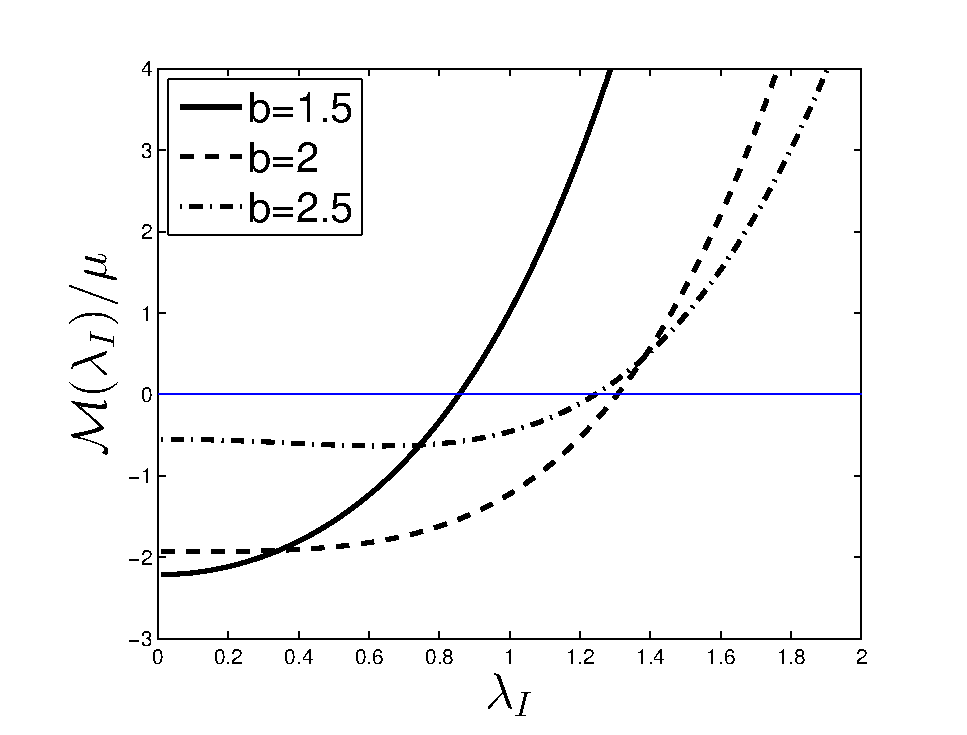
\includegraphics[width=9cm,height=4.8cm]{figs/nonlin_hopf_h.eps}
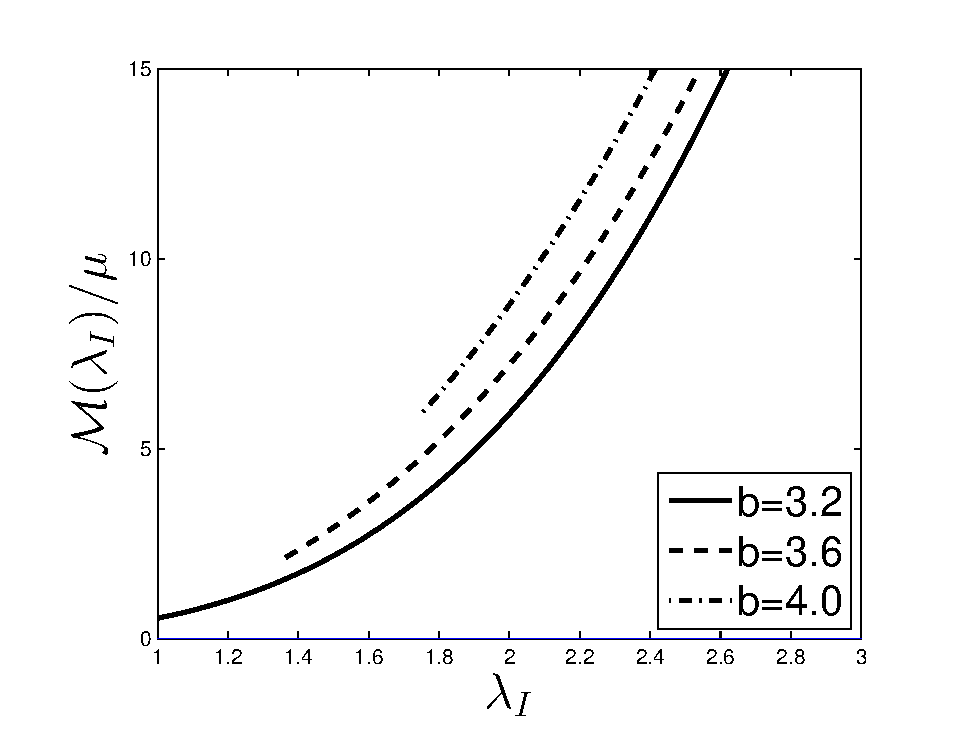
\includegraphics[width=9cm,height=4.8cm]{figs/nonlin_hopf_nh.eps}
\caption{\label{fig:nonlin} Plots of ${{\mathcal M}(\lambda_I)/\mu}$,
  where $\mu\equiv \lambda_I^2+9$, versus $\lambda_I$ for $S=6$,
  $\gamma=2$, $\alpha=1$, $U_0=4$, and $q=2$. In the left panel, where
  $b=1.5,2.0,2.5$, which satisfies $b_c<b<3$, there is a unique root
  to ${\mathcal M}(\lambda_I)=0$, yielding the Hopf eigenvalue. In the
  right panel, where $b=3.2,3.6,4.0$, there is no root to ${\mathcal
    M}(\lambda_I)=0$, and hence no Hopf eigenvalue. For our choice
  $U_0=4$, where $U_0>{3\omega/q}$, Proposition \ref{prop:genq:gap}
  gives no information regarding Hopf bifurcations on the range
  $b>3$.}
\end{figure}

To examine numerically the uniqueness of the Hopf threshold on the
range $b_c<b<3$, we take the same parameter set $S=6$, $\gamma=2$, and
$\alpha=1$, as used in \S \ref{sec:stab_q3} for the $q=3$ case. We
choose $q=2$ and $U_0=4$ for which $\eta\approx 1.286$. For $b=1.5$,
$b=2.0$, and $b=2.5$, in the left panel of Fig.~\ref{fig:nonlin} we
plot ${{\mathcal M}(\lambda_I)/\mu}$ versus $\lambda_I$ for $U_0=4$
showing numerically the existence of a unique root to ${\mathcal
  M}(\lambda_I)=0$, and consequently a unique Hopf bifurcation value
of $\hat{\tau}_{uH,j}$ for the $j$-th mode.

In contrast, suppose that $b>3$. To investigate whether a Hopf
bifurcation is possible for $3<b<{9/2}$, we must determine whether
there is a root of ${\mathcal M}(\lambda_I)=0$ on the range $\mu\equiv
9+\lambda_I^2>3b$ for which $\hat{\tau}_{u,H}>0$ (see
(\ref{param:new_tau})). From (\ref{param:nroot}), we first observe
that ${\mathcal M}(\lambda_I)=(b-3)^2\left(\eta \sqrt{3b-9} + 3b
{\mathcal F}_I(3b) \right)^2 >0$ when $\mu=3b$ and that ${\mathcal
  M}(\lambda_I)\to \infty$ as $\lambda_I\to \infty$. Therefore, if
such a root exists, ${\mathcal M}(\lambda_I)$ cannot be monotone on
$\mu>3b$. We study this issue numerically in the right panel of
Fig.~\ref{fig:nonlin} where we plot ${{\mathcal M}(\lambda_I)/\mu}$
versus $\lambda_I$ for $b=3.2$, $b=3.6$, and $b=4.0$, on the range
$\mu>3b$, for our parameter set $S=6$, $\gamma=2$, $\alpha=1$,
$U_0=4$, and $q=2$. Numerically, we find that there is no root to
${\mathcal M}(\lambda_I)=0$ when $\mu>3b$. For $U_0=4$ and $q=2$, we
remark that $U_0>{3\omega/q}$, and so Proposition \ref{prop:genq:gap}
gives no information regarding Hopf bifurcations on the range
$b>3$. Further computations (not shown) with ${\mathcal M}(\lambda_I)$
for $b>3$ suggest that there is never a root to ${\mathcal
  M}(\lambda_I)=0$ on $\mu>3b$ for any $U_0<U_{0,\max}$. Based on this
numerical evidence, we conjecture that no Hopf bifurcations can occur
when ${\mathcal D}_0<D^{-}_{0,j}$ for any $q>1$ and $U_0<U_{0,\max}$.

\begin{figure}[htbp]
\centering
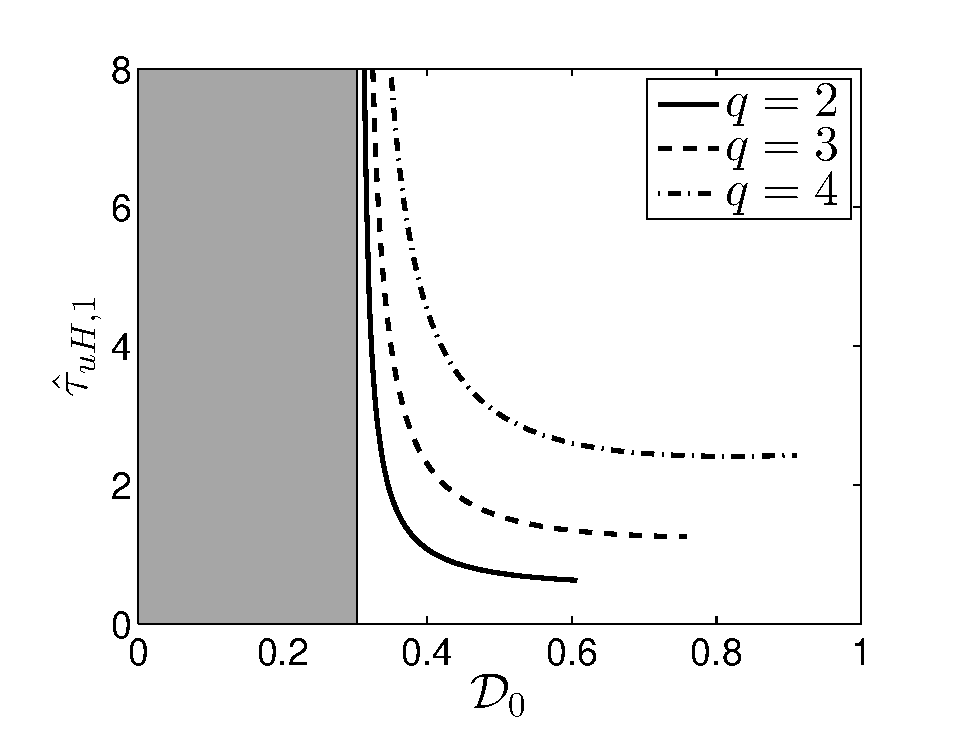
\includegraphics[width=9cm,height=4.8cm]{figs/genq_2_U02.eps}
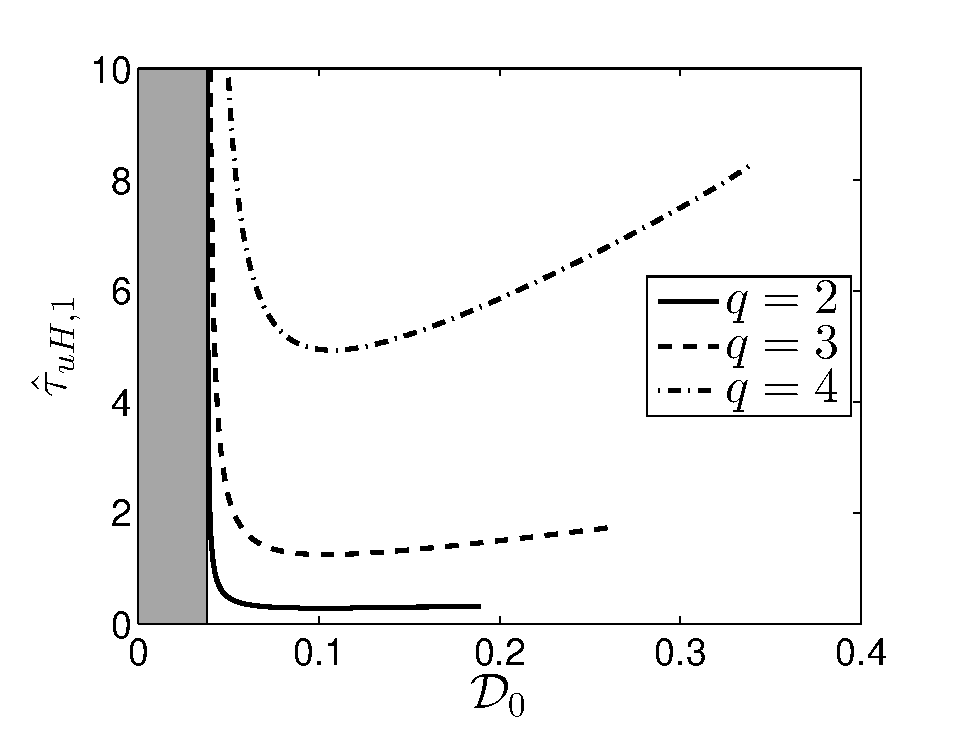
\includegraphics[width=9cm,height=4.8cm]{figs/genq_2_U04.eps}
\caption{\label{fig:genq::hopf_tau_2} The Hopf bifurcation
  threshold $\hat{\tau}_{uH_1}$ versus ${\mathcal D}_0$ for $q=2$
  (solid), $q=3$ (dashed), and $q=4$ (dot-dashed) on the range
  ${{\mathcal D}_{0,c}/(1+{qU_0/\omega})}<{\mathcal D}_0<{\mathcal
    D}_{0c}$ for $K=2$, $S=6$, $\gamma=2$, $\alpha=1$, and with
  $U_0=2$ (left panel) and $U_0=4$ (right panel). Here ${\mathcal
    D}_{0,c}$ is the competition stability threshold defined in
  (\ref{stab:zero_d0min}), which depends on $q$. The lower bound
  ${{\mathcal D}_{0,c}/(1+{qU_0/\omega})}$ is independent of $q$. The
  two-hotspot steady-state is linearly stable for ${\mathcal
    D}_0<{{\mathcal D}_{0,c}/(1+{qU_0/\omega})}$ (shaded region) as
  well as under the Hopf bifurcation curve. For ${\mathcal
    D}_0>{\mathcal D}_{0,c}$ the hotspot pattern is unstable for all
  $\hat{\tau}_u$. We observe that the interval in ${\mathcal D}_0$
  where an oscillatory instability of the hotspot amplitudes can occur
  increases with $q$. The Hopf bifurcation threshold
  $\hat{\tau}_{uH,1}$ also increases with $q$.}
\end{figure}

Next, we use our parameterization to compute the Hopf bifurcation
threshold for $\hat{\tau}_u$ on the range $D^{-}_{0,j}<{\mathcal
  D}_0<D^{+}_{0,j}$, and plot the region of linear stability for $q=2$
and $q=4$ in order to compare with our previous results in \S
\ref{sec:stab_q3} for $q=3$.

For our parameter set, and for a two-hotspot solution, in
Fig.~\ref{fig:genq::hopf_tau_2} we plot the linear stability phase
diagram in the $\hat{\tau}_u$ versus ${\mathcal D}_0$ plane when
either $U_0=2$ (left panel) and for $U_0=4$ (right panel). In both
panels we compare the linear stability thresholds for $q=2,3,4$. In
the left and right panels of Fig.~\ref{fig:genq::hopf_tau_2}, the
two-hotspot steady-state is linearly stable in the shaded region,
which is the same for each $q$, and in the region below the Hopf
bifurcation threshold for the given $q$. Since the competition
instability threshold ${\mathcal D}_{0,c}$ increases with $q$, as was
shown in \S \ref{sec:qual_comp_d}, the interval in ${\mathcal D}_0$
where an oscillatory instability of the hotspot amplitudes can occur
increases with $q$. We further observe from
Fig.~\ref{fig:genq::hopf_tau_2} that the Hopf bifurcation threshold
value of $\hat{\tau}_u$ increases with $q$, and when $U_0=4$ the Hopf
bifurcation threshold is not monotone in ${\mathcal D}_0$ when either
$q=3$ or $q=4$ (recall the right panel of Fig.~\ref{fig:hopf_tau_2}
for the $q=3$ case). These results are discussed qualitatively in
\S \ref{sec:numerics_qn3}.


For a three-hotspot pattern similar results for the linear stability
region in the $\hat{\tau}_u$ versus ${\mathcal D}_0$ plane are shown
in Fig.~\ref{fig:genq:k3:hopf_tau_U02} for $U_0=2$ and in
Fig.~\ref{fig:genq:k3:hopf_tau_U04} for $U_0=4$. Results for $q=2,3,4$
are shown in the three subpanels of these figures. We observe that the
minimal Hopf threshold value for $\hat{\tau}_u$ increases with $q$,
and this increase is more pronounced for $U_0=4$ than for $U_0=2$. For
$U_0=4$, we observe from Fig.~\ref{fig:genq:k3:hopf_tau_U04}, as
similar to that analyzed for the explicitly solvable case $q=3$ in \S
\ref{sect:q3_phase}, that when $q=4$ the minimal Hopf threshold value
for $\hat{\tau}_u$ switches between two modes at some critical ${\mathcal
  D}_0$.

Overall, our numerical results for the linear stability region for
$q=2$ and $q=4$, as computed from our parameterization
(\ref{param:all}), are qualitatively similar to those obtained from our
detailed analysis in \S \ref{sec:stab_q3} for the explicitly solvable
case $q=3$.

\begin{figure}[htbp]
\centering
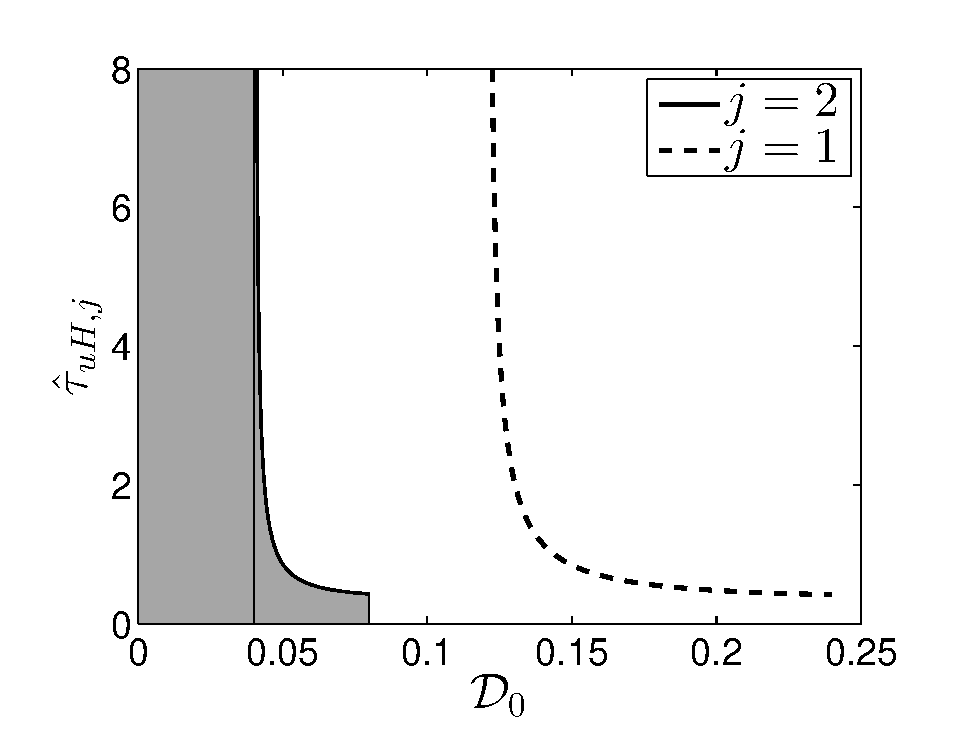
\includegraphics[width=0.32\textwidth,height=4.8cm]{figs/genq_3_q2_u02.eps}
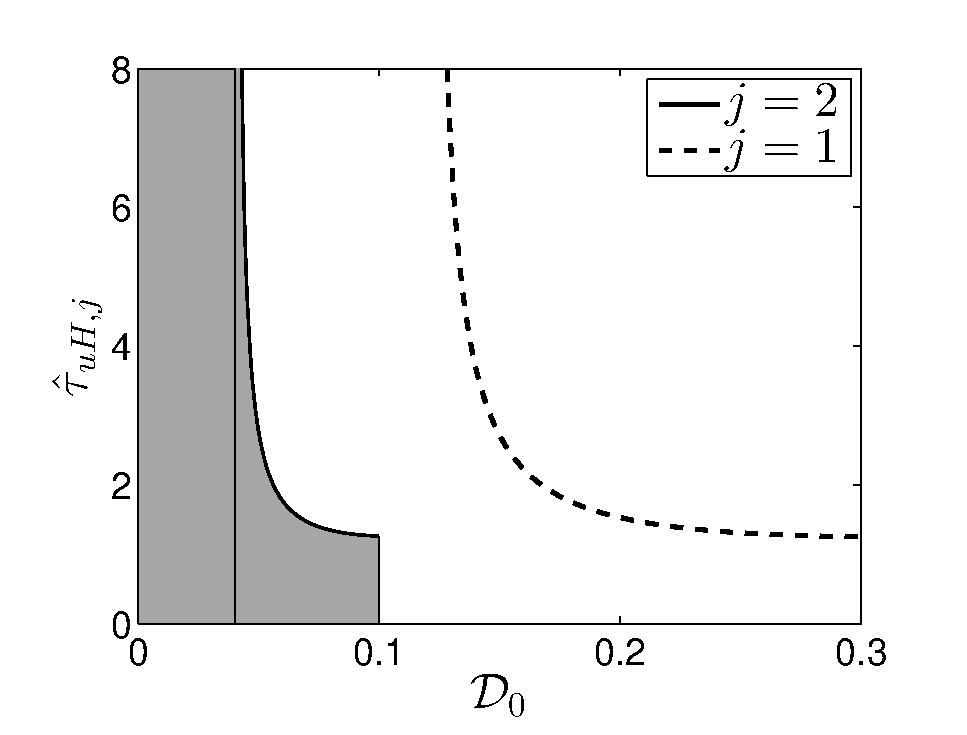
\includegraphics[width=0.32\textwidth,height=4.8cm]{figs/genq_3_q3_u02.eps}
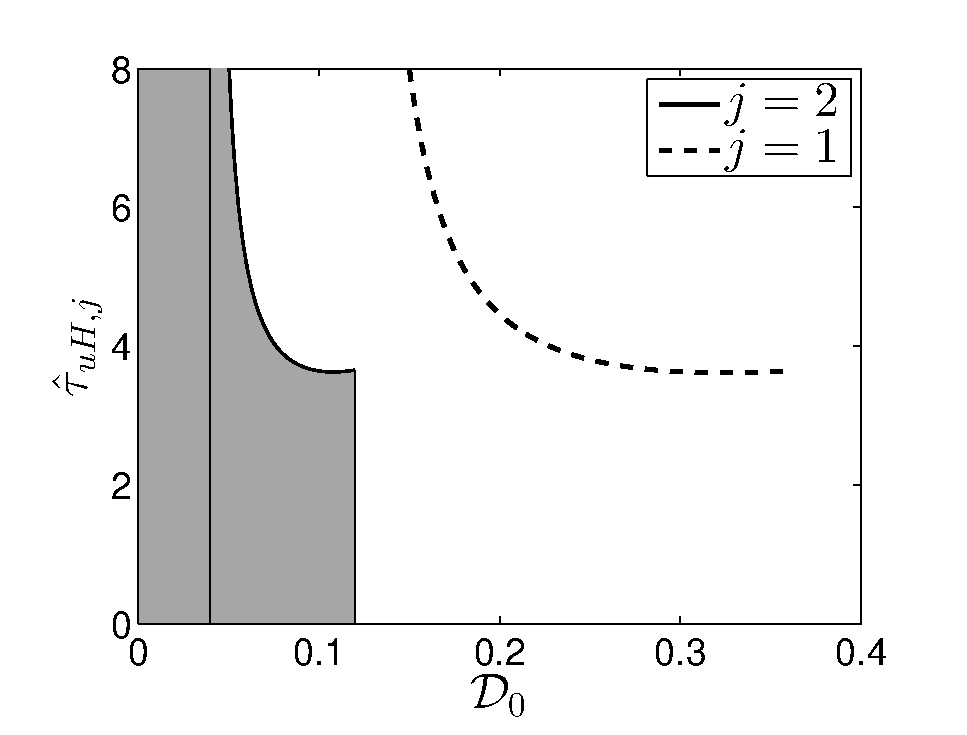
\includegraphics[width=0.32\textwidth,height=4.8cm]{figs/genq_3_q4_u02.eps}
\caption{\label{fig:genq:k3:hopf_tau_U02} Linear stability (shaded)
  region in the $\hat{\tau}_u$ versus ${\mathcal D}_0$ plane for
  $K=3$, $S=6$, $U_0=2$, $\gamma=2$ and $\alpha=1$, and for $q=2$ (left panel),
  $q=3$ (middle panel), $q=4$ (right panel). The solid and dashed
  curves are the Hopf bifurcation boundaries for the
  (sign-alternating) $j=2$ mode and the $j=1$ mode, respectively. In
  each case, the minimal Hopf boundary threshold for $\hat{\tau}_u$ is
  determined by the sign-alternating $j=2$ mode. Observe that
  $\hat{\tau}_{u,H}$ increases as $q$ increases.}
\end{figure}

\begin{figure}[htbp]
\centering
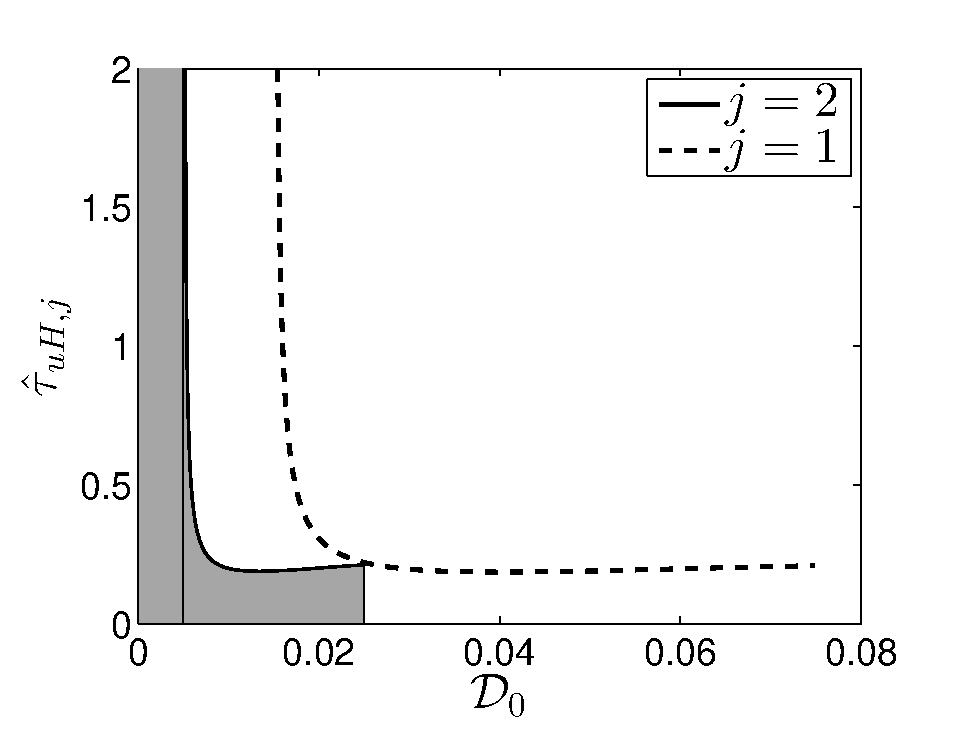
\includegraphics[width=0.32\textwidth,height=4.8cm]{figs/genq_3_q2_u04.eps}
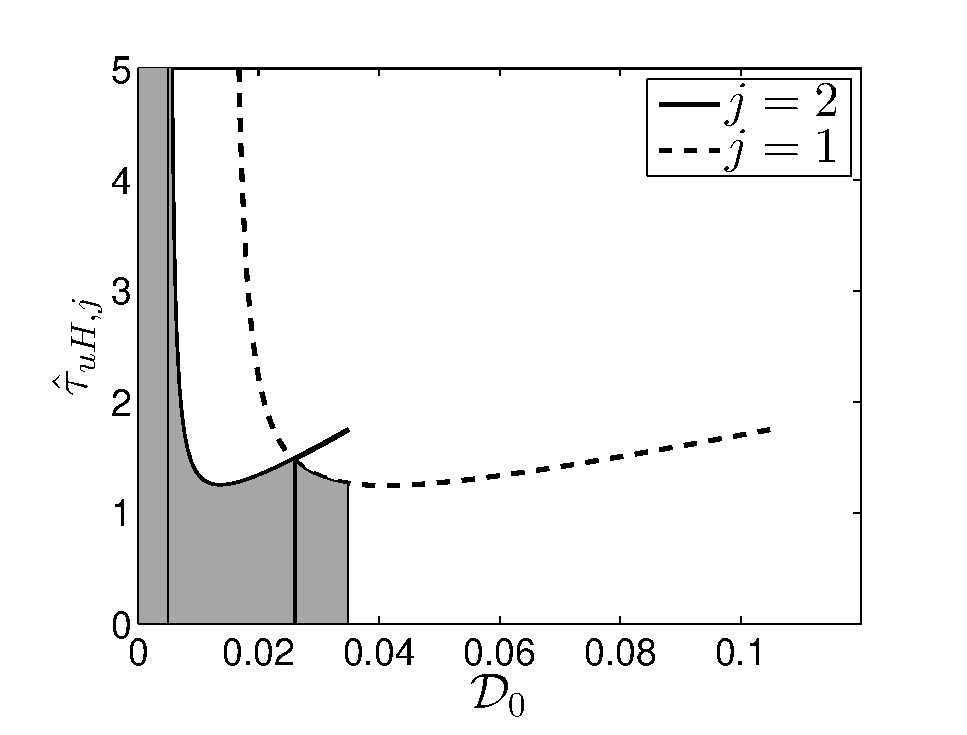
\includegraphics[width=0.32\textwidth,height=4.8cm]{figs/genq_3_q3_u04.eps}
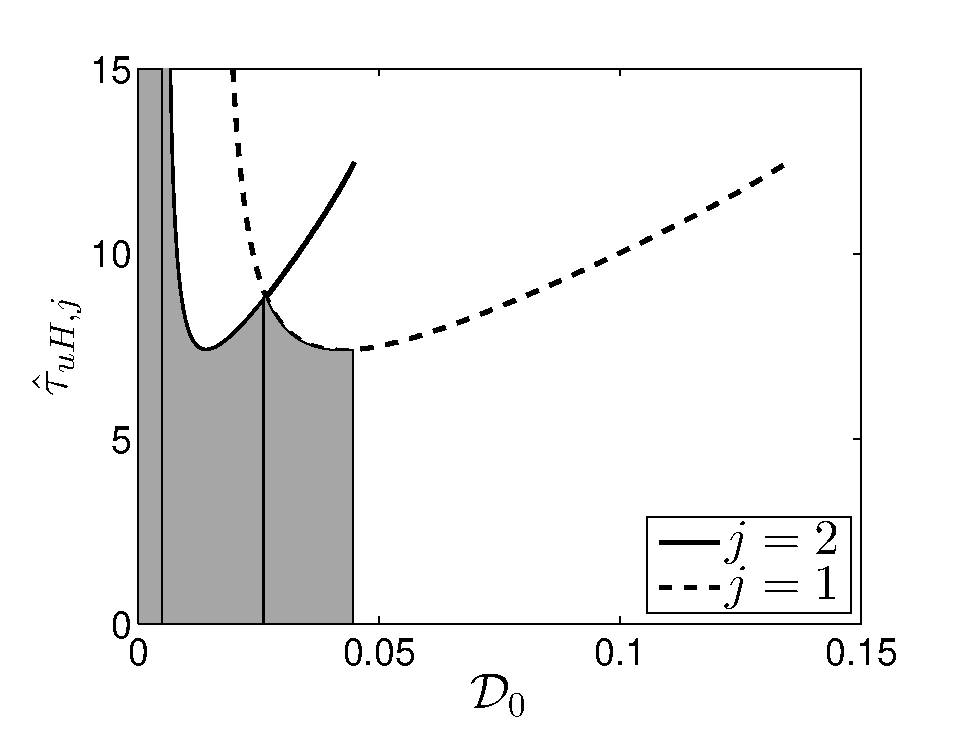
\includegraphics[width=0.32\textwidth,height=4.8cm]{figs/genq_3_q4_u04.eps}
\caption{\label{fig:genq:k3:hopf_tau_U04} Same plot and parameters as
  in Fig.~\ref{fig:genq:k3:hopf_tau_U02} except that $U_0=4$: $q=2$
  (left panel), $q=3$ (middle panel), and $q=4$ (right panel). The
  shaded region is the region of linear stability. The solid and
  dashed curves are the Hopf bifurcation boundaries for the
  (sign-alternating) $j=2$ mode and the $j=1$ mode, respectively. The
  minimal Hopf bifurcation threshold switches between the two modes
  only for $q=3$ and $q=4$. As $q$ increases the Hopf bifurcation
  threshold increases significantly (see the different vertical scales
  in the subfigures). The horizontal edge of the stability region is the
  competition stability threshold ${\mathcal D}_{0,c}$.}
\end{figure}

\subsection{Comparison of Linear Stability Theory with PDE Simulations: 
$q\neq 3$}\label{sec:numerics_qn3}


In this subsection, we validate our linear stability analysis for the
``cops-on-the-dots'' patrol strategy $q=2$ by performing full
numerical simulations of the RD system (\ref{eq:pol-main}) using the
numerical method described in \S \ref{sec:numerics_qn3}. When $q=2$,
the police diffusivity has the scaling $D_p={{\mathcal D}_0/(\epsilon
  \hat{\tau}_u)}$ and so our linear stability phase diagrams are
plotted in the $\epsilon D_p$ versus ${\mathcal D}_0$ parameter
plane. In all the results below, we use the baseline parameter set
$S=6$, $\gamma=2$, and $\alpha=1$.

\begin{figure}[htbp]
\centering
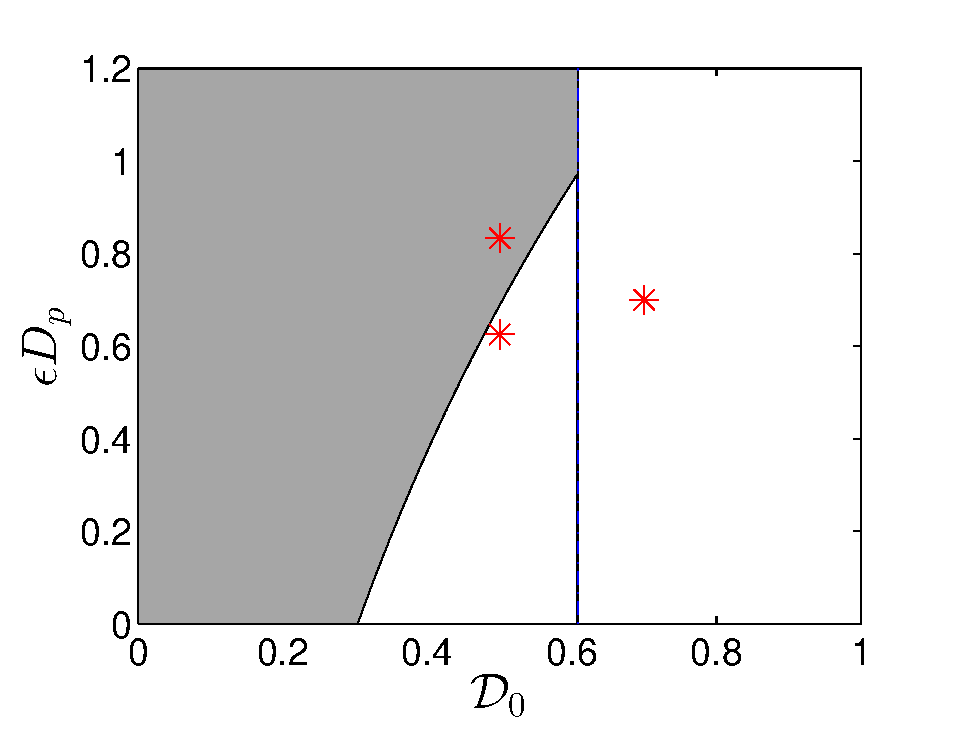
\includegraphics[width=9cm,height=4.8cm]{figs/pol_cops_2_u02.eps}
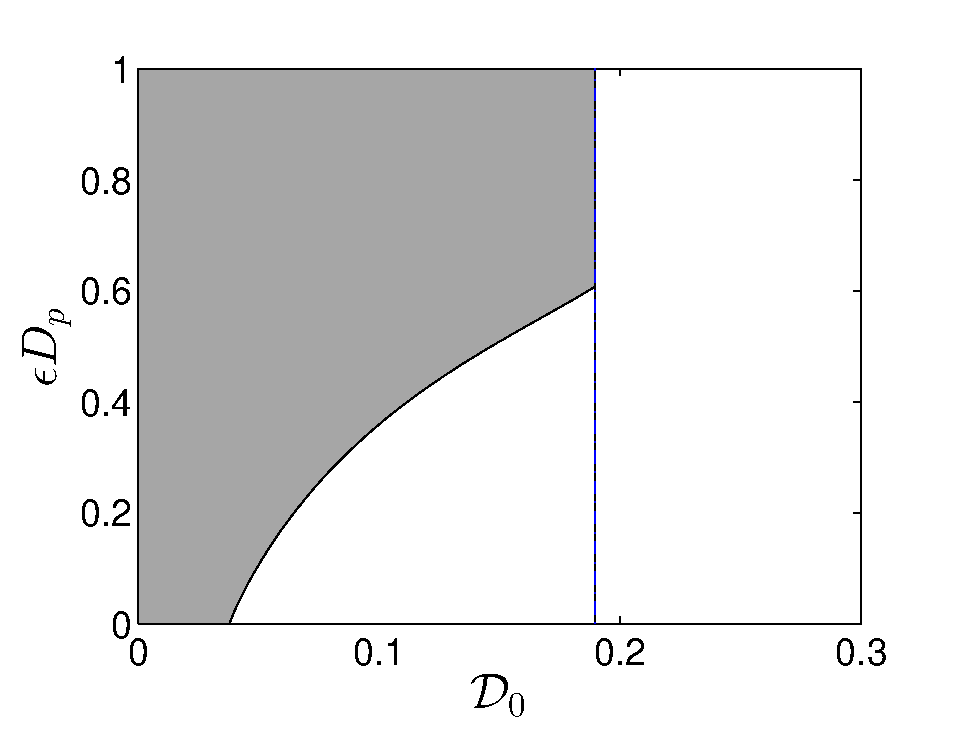
\includegraphics[width=9cm,height=4.8cm]{figs/pol_cops_2_u04.eps}
\caption{\label{fig:pol_copdots_2} Linear stability (shaded) region in
  the $\epsilon D_p$ versus ${\mathcal D}_0$ plane for a two-spot pattern
  for the $q=2$  ``cops-on-the-dots'' patrol strategy,
  with $S=6$, $\gamma=2$, and $\alpha=1$, corresponding to
  Fig.~\ref{fig:genq::hopf_tau_2}. Left panel: $U_0=2$. Right panel:
  $U_0=4$. The thin vertical line in each panel is the competition
  stability ${\mathcal D}_{0,c}$ defined in
  (\ref{stab:zero_d0min}). For ${\mathcal D}_0>{\mathcal D}_{0c}$ the
  hotspot solution is unstable due to a competition instability,
  whereas in the small unshaded region for ${\mathcal D}_0<{\mathcal
    D}_{0c}$, the hotspot steady-state is unstable to an asynchronous
  oscillatory instability of the hotspot amplitudes. The full PDE
  simulations in Fig.~\ref{fig:valid_cops_on_dots_2} are done at the
  marked points in the left panel.}
\end{figure}

For a two-hotspot pattern, the phase diagrams in the $\epsilon D_p$
versus ${\mathcal D}_0$ parameter plane corresponding to the left and
right panels of Fig.~\ref{fig:genq::hopf_tau_2} where $U_0=2$ and
$U_0=4$, respectively, are shown in Fig.~\ref{fig:pol_copdots_2}. At each
of the three marked points shown in the left panel of 
Fig.~\ref{fig:pol_copdots_2}, and with $\epsilon=0.05$,
the full numerical results for the hotspot amplitudes versus time, as
shown in the three panels of Fig.~\ref{fig:valid_cops_on_dots_2}, are
in complete agreement with the predictions of our linear stability theory.


Next, we consider a three-hotspot pattern for $q=2$ when either
$U_0=2$ or $U_0=4$, where the phase diagrams in the $\hat{\tau}_u$
versus ${\mathcal D}_0$ parameter plane are as shown in the left
panels of Fig.~\ref{fig:genq:k3:hopf_tau_U02} and
Fig.~\ref{fig:genq:k3:hopf_tau_U04}, respectively. The corresponding
linear stability phase diagrams in the $\epsilon D_p$ versus
${\mathcal D}_0$ parameter plane are shown in the left and right
panels of Fig.~\ref{fig:pol_copdots_3} for $U_0=2$ and $U_0=4$,
respectively. We now test our linear stability predictions 
at the marked points in these phase diagrams.

\begin{figure}[htbp]
\centering
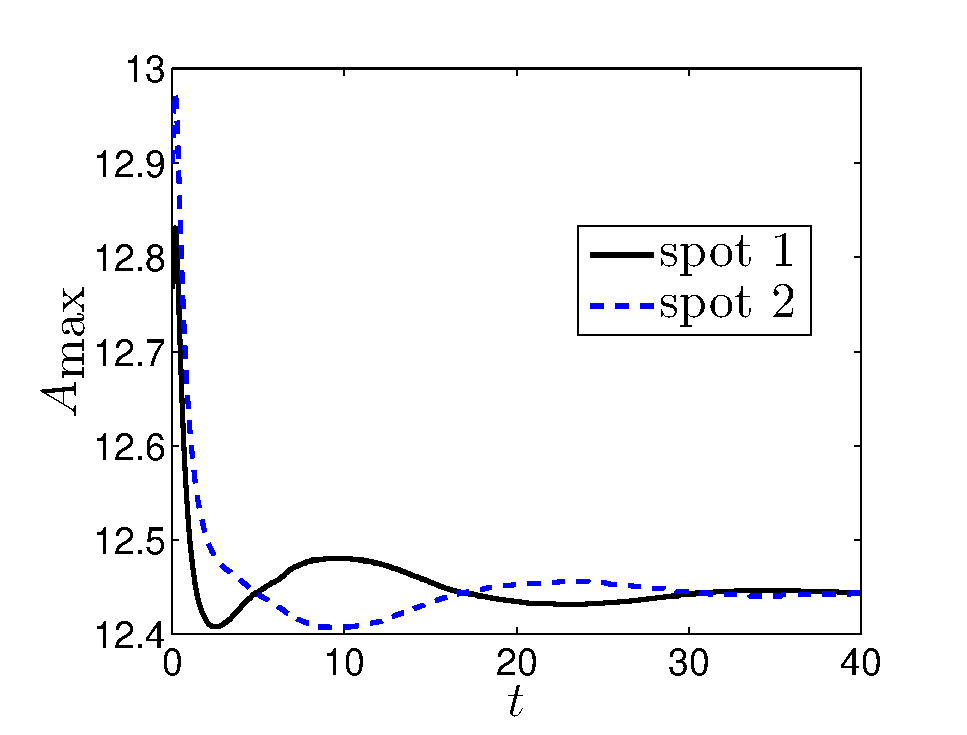
\includegraphics[width=0.32\textwidth,height=4.8cm]{figs/run1_2_q2.eps}
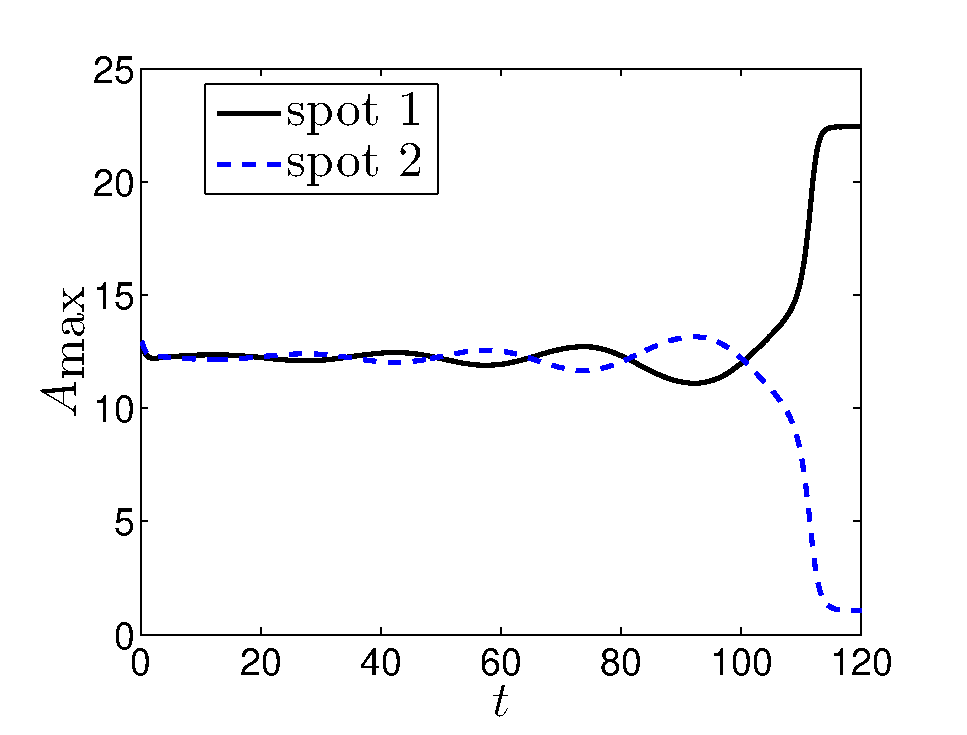
\includegraphics[width=0.32\textwidth,height=4.8cm]{figs/run2_2_q2.eps}
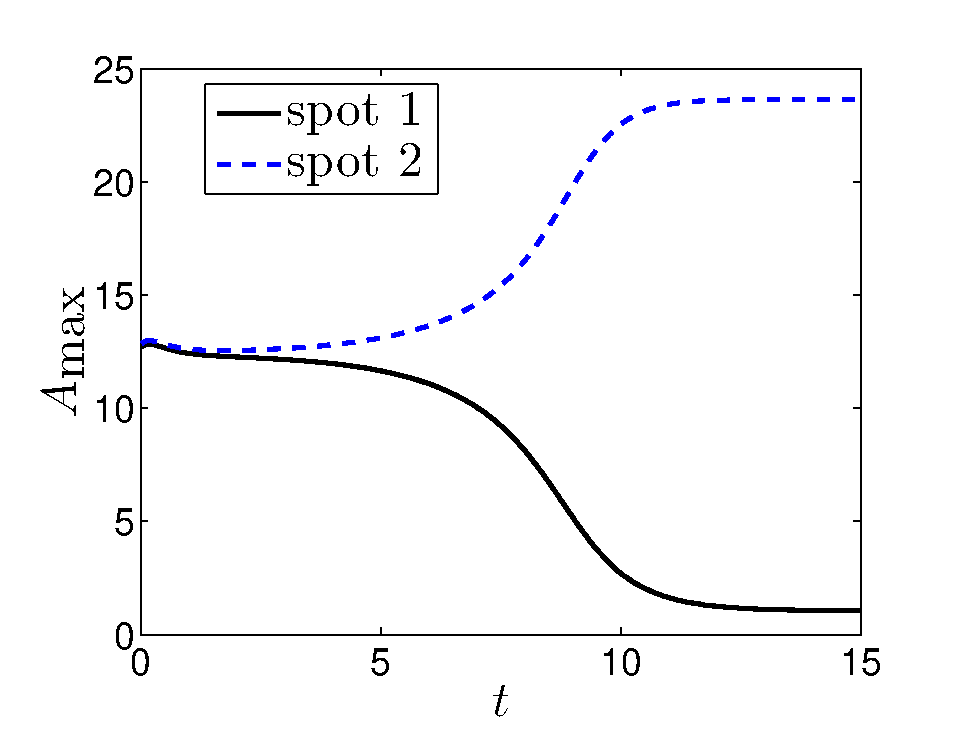
\includegraphics[width=0.32\textwidth,height=4.8cm]{figs/run3_2_q2.eps}
\caption{\label{fig:valid_cops_on_dots_2} The spot amplitudes
  computed numerically from the full PDE system (\ref{eq:pol-main})
  for a two-spot pattern for the $q=2$ ``cops-on-the-dots'' patrol
  strategy, and with $S=6$, $\gamma=2$, $\alpha=1$, $U_0=2$, and
  $\epsilon=0.05$. These simulations at the marked points in the phase
  diagram in the left panel of Fig.~\ref{fig:pol_copdots_2} confirm
  our linear stability theory.  Left panel: $\hat{\tau}_u=0.6$ and
  ${\mathcal D}_0=0.5$, so that $\epsilon D_p\approx 0.833$. The
  asynchronous spot amplitude oscillations decay in time. Middle
  panel: $\hat{\tau}_u=0.8$ and ${\mathcal D}_0=0.5$, so that
  $\epsilon D_p = 0.625$. The asynchronous spot amplitude
  oscillations grow in time and lead to the collapse of a spot. When
  ${\mathcal D}_0=0.5$, the Hopf bifurcation threshold is
  $\epsilon D_{p,H} \approx 0.6887$ (see the left panel of
  Fig.~\ref{fig:pol_copdots_2}). Right panel: $\hat{\tau}_u=1.0$ and
  ${\mathcal D}_0=0.7$, so that $\epsilon D_p=0.7$. The
  competition instability for the spot amplitudes leads to the
  collapse of a spot.}
\end{figure}


We first consider the three marked points shown in the left panel of
Fig.~\ref{fig:pol_copdots_3}, where $U_0=2$.  For $\epsilon=0.035$,
the full numerical results for the hotspot amplitudes versus time, are
shown in the three panels of Fig.~\ref{fig:valid_cops_on_dots_3}. In
the left and middle panels of Fig.~\ref{fig:valid_cops_on_dots_3},
which correspond to parameter values either slightly below or slightly above
our theoretically predicted Hopf bifurcation threshold, we observe either
slowly decaying or growing sign-alternating asynchronous oscillations as
predicted by our linear stability theory. These two parameter values 
correspond to the two closely spaced points in the phase diagram in the 
left panel of Fig.~\ref{fig:pol_copdots_3}. Moreover, the right panel of
Fig.~\ref{fig:valid_cops_on_dots_3} clearly illustrates the competition
instability which occurs for the marked point in the left panel of
Fig.~\ref{fig:pol_copdots_3} with ${\mathcal D}_0>{\mathcal D}_{0,c}$.


\vfill\eject

\begin{figure}[htbp]
\centering
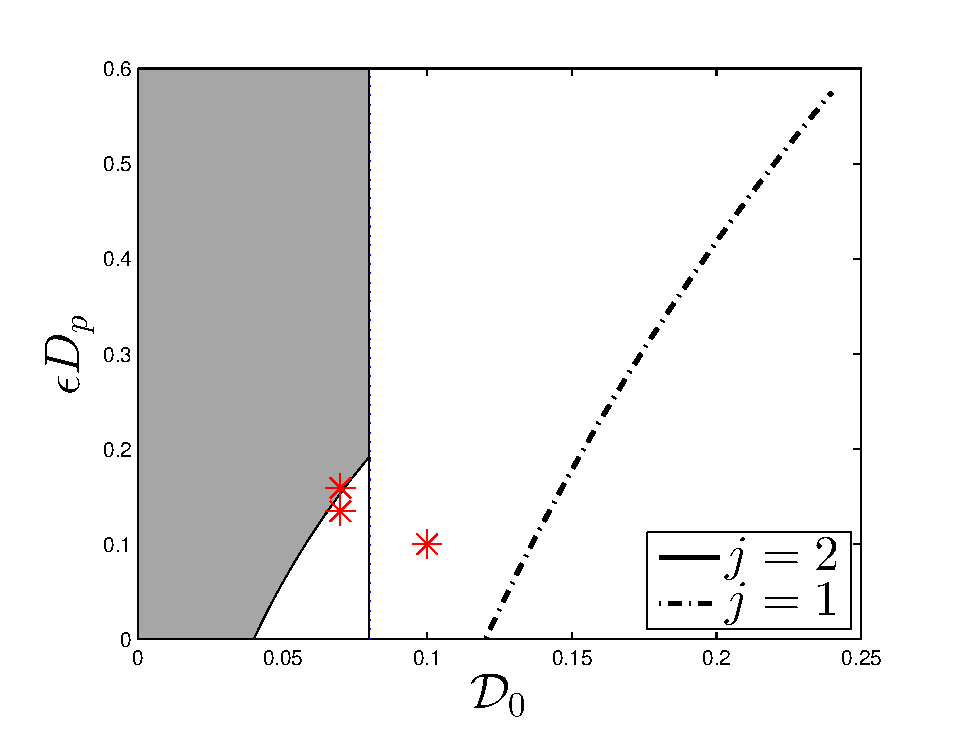
\includegraphics[width=9cm,height=4.8cm]{figs/pol_cops_3_u02.eps}
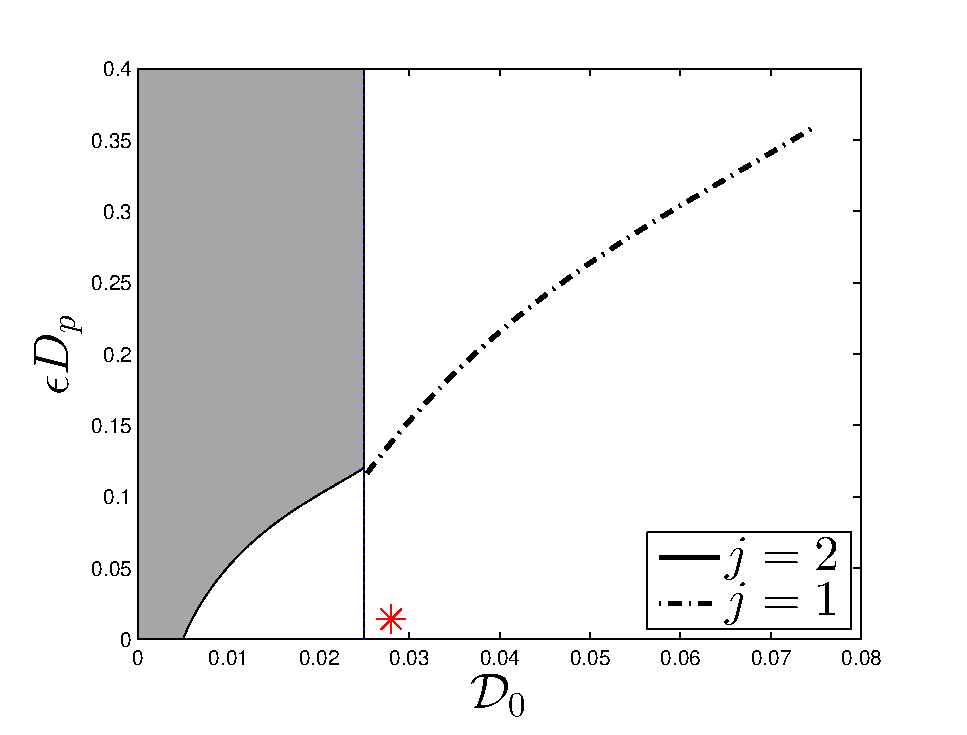
\includegraphics[width=9cm,height=4.8cm]{figs/pol_cops_3_u04.eps}
\caption{\label{fig:pol_copdots_3} Linear stability (shaded) region in
  the $\epsilon D_p$ versus ${\mathcal D}_0$ plane for a three-spot
  pattern for the $q=2$ ``cops-on-the-dots'' patrol strategy, with
  $S=6$, $\gamma=2$, and $\alpha=1$ and for $U_0=2$ (left panel) and
  $U_0=4$ (right panel). Plots correspond to the left panels of
  Fig.~\ref{fig:genq:k3:hopf_tau_U02} and
  Fig.~\ref{fig:genq:k3:hopf_tau_U04}. The competition instability
  threshold is the thin vertical line. The solid and dot-dashed curves
  are the Hopf bifurcation boundaries for the (sign-alternating) $j=2$
  mode and the $j=1$ mode, respectively. For both $U_0=2$ and $U_0=4$,
  the Hopf boundary for ${\mathcal D}_0<{\mathcal D}_{0,c}$, marking
  the boundary of the small unshaded region, is determined by the
  sign-altering $j=2$ mode.  The full PDE simulations in
  Fig.~\ref{fig:valid_cops_on_dots_3} and in 
  Fig.~\ref{fig:valid_cops_on_dots_3_b} are done at the marked point(s)
  in the left and right panels.}
\end{figure}

\begin{figure}[htbp]
\centering
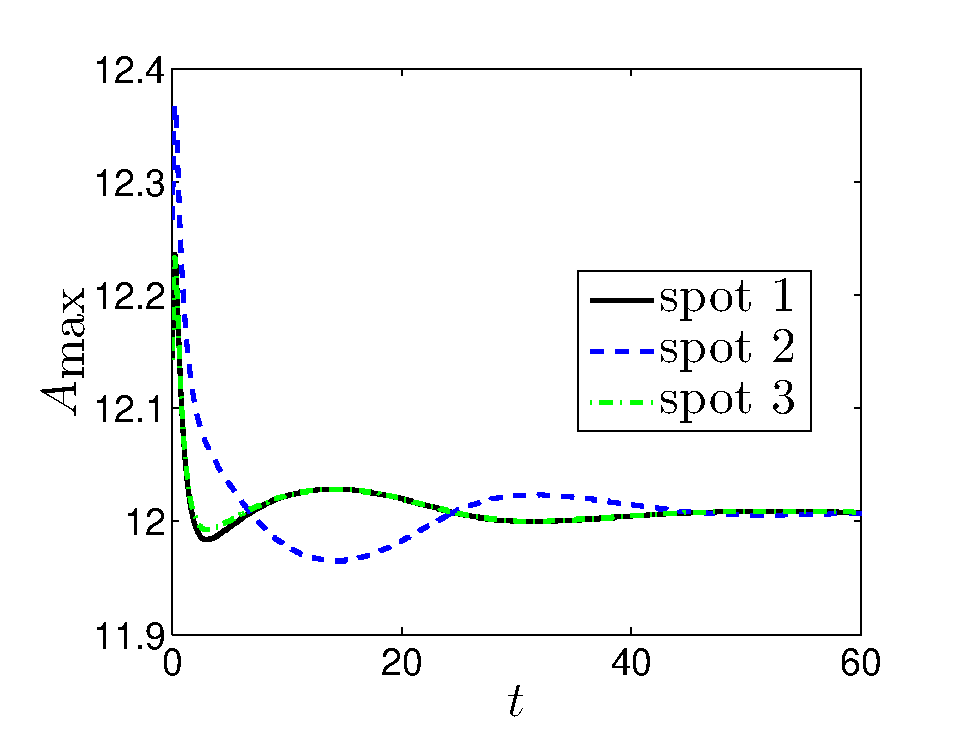
\includegraphics[width=0.32\textwidth,height=4.8cm]{figs/run1_3_q2.eps}
\includegraphics[width=0.32\textwidth,height=4.8cm]{figs/run2_3_q2.eps}
\includegraphics[width=0.32\textwidth,height=4.8cm]{figs/run3_3_q2.eps}
\caption{\label{fig:valid_cops_on_dots_3} The spot amplitudes
  computed numerically from the full PDE system (\ref{eq:pol-main})
  for a three-spot pattern for the $q=2$ ``cops-on-the-dots'' patrol
  strategy, and with $S=6$, $\gamma=2$, $\alpha=1$, $U_0=2$, and
  $\epsilon=0.035$. These simulations at the marked points in the left
  panel of Fig.~\ref{fig:pol_copdots_3} confirm
  our linear stability theory.  Left panel: $\hat{\tau}_u=0.44$ and
  ${\mathcal D}_0=0.07$, so that $\epsilon D_p\approx 0.159$. The
  asynchronous spot amplitude oscillations decay in time. Middle
  panel: $\hat{\tau}_u=0.52$ and ${\mathcal D}_0=0.07$, so that
  $\epsilon D_p = 0.1346$. The asynchronous spot amplitude
  oscillations grow in time and lead to the collapse of a spot. When
  ${\mathcal D}_0=0.07$, the Hopf bifurcation threshold is
  $\epsilon D_{p,H} \approx 0.1532$ (see the left panel of
  Fig.~\ref{fig:pol_copdots_3}). Right panel: $\hat{\tau}_u=1.0$ and
  ${\mathcal D}_0=0.1$, so that $\epsilon D_p=0.1$. The
  competition instability for the spot amplitudes leads to the
  collapse of a spot.}
\end{figure}

Finally, as a more refined test of our linear stability theory, we
perform full numerical simulations for the marked point in the phase
diagram shown in the right panel of Fig.~\ref{fig:pol_copdots_3} where
$U_0=4$. This stability phase diagram predicts that the three-spot
pattern is unstable to both a competition instability and a $j=1$ mode
asynchronous oscillatory instability, representing anti-phase
oscillations between the first and third hotspots. However, the
unstable real eigenvalue associated with the competition instability
is rather close to the origin of the spectral plane since ${\mathcal
  D}_0$ is only slightly above the competition threshold ${\mathcal
  D}_{0,c}$. As such, we predict that the anti-phase oscillation
should be the more dominant of the two instabilities. This anti-phase
oscillation is clearly evident from the full PDE simulation shown in
Fig.~\ref{fig:valid_cops_on_dots_3_b} when $\epsilon=0.035$.

\begin{figure}[htbp]
\centering
\includegraphics[width=0.450\textwidth,height=4.8cm]{figs/run4_3_q2.eps}
\caption{\label{fig:valid_cops_on_dots_3_b} The numerically computed
  spot amplitudes at the marked point in the right panel of
  Fig.~\ref{fig:pol_copdots_3} for $U_0=4$, where ${\mathcal
    D}_0=0.028$, $\hat{\tau}_u=2$, so that $\epsilon D_p\approx
  0.014$. The other parameters are $S=6$, $\gamma=2$, $\alpha=1$, and
  $\epsilon=0.035$. The phase diagram in the right panel of
  Fig.~\ref{fig:pol_copdots_3} predicts that the three-spot pattern is
  unstable to a competition instability together with a $j=1$ mode
  anti-phase oscillatory instability between the first and third
  spots. Since ${\mathcal D}_0\approx {\mathcal D}_{0,c}$, the
  competition instability should be weak, and so the anti-phase
  oscillation is predicted to be the more dominant of the two
  instabilities. This is confirmed by the full PDE simulation.}
\end{figure}
 
\setcounter{equation}{0}
\setcounter{section}{7}
\section{Discussion and Outlook}\label{sec:disc}

We have used a combination of matched asymptotic expansions and the
analysis of nonlocal eigenvalue problems (NLEP) to study the existence
and linear stability of localized hotspot steady-state solutions for
the three-component RD system (\ref{eq:crs-main}) in the limit
$\epsilon\to 0$ with $D={{\mathcal D}_0/\epsilon^2}$ on the 1-D domain
$0\leq x\leq S$. We have investigated how the multiple hotspot
steady-states and their linear stability properties depend on the
total police deployment $U_0>0$, the patrol focus parameter $q>1$, and
the police diffusivity $D_p\equiv {{\mathcal D}_0/\eps^2 \tau_u}$, where
$\tau_u=\epsilon^{q-3}\hat{\tau}_u$ with $\hat{\tau}_u={\mathcal
  O}(1)$.

Our NLEP linear stability analysis has provided phase diagrams in the
$\epsilon^{q-1} D_{p}$ versus ${\mathcal D}_0$ parameter space where
multiple hotspot steady-states are linearly stable. We have shown that
the hotspot amplitudes are always linearly stable to synchronous
perturbations of their amplitudes. Instabilities can only arise from
the asynchronous modes, which decrease the amplitudes of certain
hotspots at the expense of increasing the intensity of others. For the
special case $q=3$, and for $K\geq 2$, for which the discrete spectrum
of the NLEP can be reduced to the study of a family of $K-1$ quadratic
equations in the eigenvalue parameter, stability phase-diagrams in the
$\epsilon^{2} D_p$ versus ${\mathcal D}_0$ parameter plane were constructed
explicitly. For general $q>1$, the phase diagrams were determined by
combining some rigorous spectral results obtained from the argument
principle together with numerical results obtained from a
parameterization of the Hopf bifurcation threshold.

Our hybrid anayltical-numerical study has shown that steady-state
multiple hotspot patterns are unconditionally unstable if ${\mathcal
  D}_0>{\mathcal D}_{0,c}$, and are always linearly stable if
$0<{\mathcal D}_0< {\mathcal D}_{0,c}/(1+qU_0/\omega)$, where
$\omega=S(\gamma-\alpha)-U_0$ and ${\mathcal D}_{0,c}$ is the
competition instability threshold given in (\ref{stab:zero_d0min}). On
the intermediate range ${\mathcal D}_{0,c}/(1+qU_0/\omega)<{\mathcal
  D}_0<{\mathcal D}_{0,c}$, we have shown from an analysis of the NLEP
that the hotspot amplitudes exhibit an asynchronous oscillatory
instability of their amplitudes due to a Hopf bifurcation when the
police diffusivity $D_p$ is below a certain threshold, which depends
on ${\mathcal D}_0$. Therefore, for this range of ${\mathcal D}_0$, a
sufficiently ``sluggish'' police intervention has the effect of only
displacing crime between adjacent hotspots. The specific asynchronous
spatial mode for this displacement depends on the level of police
deployment $U_0$. For $U_0$ small enough, the sign-alternating
asynchronous mode was shown to be the dominant oscillatory
instability.

We conclude this paper by briefly discussing a few problems that
warrant further study.

From a mathematical viewpoint, there are some open theoretical
questions for our RD system (\ref{eq:pol-main}). Firstly, for a
general $q>1$, our result in Proposition \ref{prop:genq:gap} proves
that the NLEP (\ref{stab:nlep_final_1}) has no unstable eigenvalues on
the entire range ${\mathcal D}_0<{\mathcal
  D_{0,c}/\left(1+{qU_0/\omega}\right)}$, where
$\omega=S(\gamma-\alpha)-U_0>0$, only when the total police deployment
$U_0$ satisfies $U_0<{2S(\gamma-\alpha)/(q+1)}$. Although our
numerical evidence obtained from the Hopf threshold parameterization
(\ref{param:all}) supports a conclusion that the NLEP has no unstable
eigenvalues on the entire range ${\mathcal D}_0<{\mathcal
  D_{0,c}/\left(1+{qU_0/\omega}\right)}$ for any $0<U_0<U_{0,\max}$
and $q>1$, it would be worthwhile to prove this result rigorously. For
the explicitly solvable case $q=3$, such a rigorous proof was done in
\S \ref{sec:stab_q3}. Secondly, our analysis of steady-state hotspot
patterns and their stability properties is not valid when
$q=1$. Qualitatively, for $q=1$, the police are less focused on maxima
of $A$ than are the criminals, so that the density of police remains
at a significant level near the peripheries of a hotspot region. Such
a policing strategy is related to the concept of peripheral
interdiction, as discussed in \cite{jbc}. Mathematically, for $q=1$,
we need to modify our steady-state hotspot construction as well as
modify the derivation of the underlying NLEP. This latter fact follows
since for $q=1$ we have $\hat{\tau}_{u} =\epsilon^{2}\tau_{u}$ from
(\ref{eq:pol-tau-hat}), so that the ODE for the perturbation $\eta$ in
(\ref{stab:out_eta}) now satisfies ${\mathcal
  D}_{0}\eta_{xx}=\hat{\tau}_u\lambda\eta\,.$ As such, the expression
for $\eta(0)$ in (\ref{eq:pol-eta_0-1}) is no longer valid. As a
result, we will obtain a modified NLEP problem, distinct from that in
(\ref{stab:nlep_final_1}), which will require a separate analysis.
Intuitively, we might expect that a $q=1$ peripheral-based policing
strategy will act to decrease the parameter range where asynchronous
temporal instabilities in the hotspot amplitudes can occur.  Thirdly,
we emphasize that our analysis has been based on using NLEP theory to
examine the linear instability mechanisms on an ${\mathcal O}(1)$
time-scale of symmetric steady-state hotspot patterns. As an extension
to our NLEP analysis, one should examine the role of the ``small''
eigenvalues in the spectrum of the linearization that tend to zero
$\epsilon\to 0$. Zero-crossings of these small eigenvalues should
correspond to bifurcation points where asymmetric hotspot
steady-states bifurcate from the steady-state symmetric solution
branch.  Lastly, it would be interesting to develop a weakly nonlinear
analysis to establish whether both the competition instability and the
Hopf bifurcation for the asynchronous mode are subcritical. The full
PDE numerical simulations shown in \S \ref{sec:numerics_q3} and in \S
\ref{sec:numerics_qn3} support this conjecture in that small-scale
asynchronous oscillations appear to trigger a nonlinear process
through which one or more hotspots are ultimately annihilated.

Finally, we discuss a few possible extensions of the analysis and the
model of police interactions. For the RD system (\ref{eq:pol-main}) it
would be interesting to study hotspot patterns for the regime where
$D={\mathcal O}(1)$. For the basic two-component crime model with no
police intervention, it was shown in \cite{tw} that near a saddle-node
bifurcation point for hotspot equilibria there can be a nucleation of
new hotspots of criminal activity from an otherwise quiescent, largely
crime-free, background. In this direction it would be interesting to
investigate whether the police presence can eliminate this
``peak-insertion'' effect, and more generally how the global
bifurcation behavior of multiple hotspot steady-state solutions is
modified due to the police.  A second open area is to study the
existence and linear stability properties of hotspot patterns for our
three-component RD system in a 2-D spatial domain in order to
determine whether the police intervention can lead to asynchronous
temporal oscillations in the hotspot amplitudes, which model the
displacement of crime between various localized spatial regions.
Finally, it would be interesting to consider a more general model for
police intervention whereby the police interaction $I$ on the criminal
density is modeled by the ``predator-prey'' interaction
$I(U,\rho)=-U\rho$ rather than simply $I=-U$ as we have done.  The
NLEP characterizing the linear stability of steady-state symmetric
hotspot patterns on an ${\mathcal O}(1)$ time-scale will now have
three, instead of two, nonlocal terms, which makes a detailed
stability analysis rather challenging. However, the determination of
the competition instability threshold, corresponding to the
zero-eigenvalue crossing, should be feasible.

\appendix

\section{The Continuum Limit of the Agent-Based Model} 

\section*{Acknowledgments}
M.~J.~Ward was supported by the NSERC Discovery Grant 81541. We
gratefully acknowledge helpful discussions with Prof.~Theodore
Kolokolnikov and Prof.~Juncheng Wei on the NLEP analysis.

\begin{thebibliography}{99}

%\bibitem{bn} H.~Berestycki, J.-P.~Nadal, \textit{Self-organised
%critical hot spots of criminal activity}, Europ. J. Appl. Math.,
%\textbf{21}(4-5), (2010), pp.~371--399.

%done
\bibitem{bww} H.~Berestycki, J.~Wei, M.~Winter, \textit{Existence
of symmetric and asymmetric spikes for a crime hotspot model}, SIAM
J. Math. Anal., \textbf{46}(1), (2014), pp.~691--719.

%done
\bibitem{vlug} J.~G.~Blom, R.~A.~Trompert, J.~G.~Verwer,
\textit{Algorithm 758: VLUGR 2: A vectorizable adaptive grid solver for
PDEs in 2D}, ACM Trans, Math. Softw., \textbf{22}(3), (1996), pp.~302--328.

%done
\bibitem{braga} A.~A.~Braga, \textit{The effects of hot spots policing
  on crime}, Ann. Am. Acad. Polit. S. S., \textbf{578}, (2001),
  pp.~104--125.

%done
\bibitem{bb} P.~L.~Brantingham, P.~J.~Brantingham, \textit{Crime
patterns}, McMillan, (1987).

%done
\bibitem{smith} A.~Camacho, H.~R.~L.~Lee, L.~Smith, \textit{Modeling policing
strategies for departments with limited resources}, Europ. J. Appl. Math.,
\textbf{27}(3), (2016). pp.~479--501.

%done
\bibitem{ccm} R.~Cantrell, C.~Cosner, R.~Manasevich, \textit{Global
  bifurcation of solutions for crime modeling equations}, SIAM
  J. Math. Anal., \textbf{44}(3), (2012), pp.~1340--1358.

%done
\bibitem{dgk_0} A.~Doelman, R.~A.~Gardner, T.~J.~Kaper, \textit{Large
  stable pulse solutions in reaction-diffusion equations}, Indiana
  U. Math. J., \textbf{50}(1), (2001), pp.~443--507.

%done
\bibitem{GWY} Y.~Gu, Q.~Wang, G.~Yi, \textit{Stationary
patterns and their selection mechanism of urban crime models with
heterogeneous near-repeat victimization effect}, Europ. J. Appl.
Math., \textbf{28}(1), (2017), pp.~141--178.

%done
\bibitem{iww} D.~Iron, M.~J.~Ward, J.~Wei, \textit{The
stability of spike solutions to the one-dimensional Gierer-Meinhardt
model}, Physica D, \textbf{150}(1-2), (2001), pp.~25--62.

%done
\bibitem{jb} S.~Johnson, K. Bower, \textit{Domestic burglary
repeats and space-time clusters: The dimensions of risk}, Europ. J.
of Criminology, \textbf{2}, (2005), pp.~67--92.

\bibitem{jbc} P.~A.~Jones, P.~J.~Brantingham, L.~Chayes,
  \textit{Statistical models of criminal behavior: The effect of law
    enforcement actions}, Math. Models. Meth. Appl. Sci., \textbf{20},
  Suppl., (2010), pp.~1397--1423.

%done
\bibitem{kww_crime} T.~Kolokolnikov, M.~J.~Ward, J.~Wei, \textit{The
  stability of steady-state hot-spot patterns for a reaction-diffusion
  model of urban crime}, DCDS-B, \textbf{19}(5), (2014),
  p.~1373--1410.

%done
\bibitem{mk_mesa} R.~McKay, T.~Kolokolnikov, \textit{Stability
  transitions and dynamics of localized patterns near the shadow limit
  of reaction-diffusion systems}, DCDS-B, \textbf{17}(1), (2012)
  pp.~191--220.

%done
\bibitem{kww_gs} T.~Kolokolnikov, M.~J.~Ward, J.~Wei, \textit{The 
   existence and stability of spike equilibria in the one-dimensional 
   Gray-Scott model: The low feed rate regime}, Studies in Appl.
   Math, \textbf{115}(1), (2005), pp.~21--71.

%done
\bibitem{kw_xdiff} T.~Kolokolnikov, J.~Wei, \textit{Stability
of spiky solutions in a competition model with cross-diffusion}, SIAM
J. Appl. Math., \textbf{71}(4), (2011), pp. 1428--1457.

%done
\bibitem{lf} D.~J.~B.~Lloyd, H.~O'Farrell, \textit{On
  localised hotspots of an urban crime model}, Physica D,
  \textbf{253}, (2013), pp.~23--39.

%done
\bibitem{mtw_enlep} I.~Moyles, W.-H.~Tse, M.~J.~Ward,
  \textit{Explicitly solvable nonlocal eigenvalue problems and the
    stability of localized stripes in reaction-diffusion systems},
  Studies in Appl. Math., \textbf{136}(1), (2016), pp.~89--136.

%done
\bibitem{nec} Y.~Nec, M.~J.~Ward, \textit{An explicitly solvable
nonlocal eigenvalue problem and the stability of a spike for a class
of reaction-diffusion system with sub-diffusion}, Math. Model. of
Nat. Phenom., \textbf{8}(2), (2013), pp. 55--87.

%done
\bibitem{nec_sub} Y.~Nec, M.~J.~Ward, \textit{The dynamics and stability of 
spike-type solutions to the Gierer-Meinhardt model with sub-diffusion},
Physica D, \textbf{241}(10), (2012), pp.~947--963.

%done
\bibitem{floq-ref} H.~van der Ploeg, A.~Doelman, \textit{
  Stability of spatially periodic pulse patterns in a class of
  singularly perturbed reaction-diffusion equations}, Indiana
  Univ. Math. J., \textbf{54}(5), (2005), pp.~1219--1301

\bibitem{pitcher} A.~B.~Pitcher, \textit{Adding police to a
  mathematical model of burglary}, Europ. J. Appl. Math.,
  \textbf{21}(4-5), (2010), pp.~401--419.

\bibitem{rick} L.~Ricketson, \textit{A continuum model of residential
  burglary incorporating law enforcement}, unpublished,
  (2011). Retrieved from
  http://cims.nyu.edu/\textasciitilde{}lfr224/writeup.pdf.

%done
\bibitem{rb} N.~Rodriguez, A.~Bertozzi, \textit{Local existence and
  uniqueness of solutions to a PDE model for criminal behavior}, M3AS
  (special issue on Mathematics and Complexity in Human and Life
  Sciences), \textbf{20}(1), (2010), pp.~1425--1457.

%done
\bibitem{RRW} I.~Rozada, S.~Ruuth, M.~J.~Ward, \textit{The stability of
 localized spot patterns for the Brusselator on the sphere}, SIAM J. Appl. 
Dyn. Sys., \textbf{13}(1), (2014), pp.~564--627.

%done
\bibitem{s_1} M.~B.~Short, M.~R.~D'Orsogna, V.~B.~Pasour, G.~E.~Tita,
  P.~J.~Brantingham, A.~L.~Bertozzi, L.~B.~Chayes, \textit{A
    statistical model of criminal behavior}, Math. Models. Meth. Appl.
  Sci., \textbf{18}, Suppl., (2008), pp.~1249--1267.

%done
\bibitem{s_2} M.~B.~Short, A.~L.~Bertozzi, P.~J.~Brantingham
  \textit{Nonlinear patterns in urban crime - hotspots, bifurcations,
    and suppression}, SIAM J. Appl. Dyn. Sys., \textbf{9}(2), (2010),
  pp.~462--483.

%done
\bibitem{s_3} M.~B.~Short, P.~J.~Brantingham, A.~L.~Bertozzi,
  G.~E.~Tita (2010), \textit{Dissipation and displacement of hotpsots
    in reaction-diffusion models of crime}, Proc. Nat. Acad. Sci.,
  \textbf{107}(9), pp.~3961-3965.

%done
\bibitem{tw} W.-H.~Tse, M.~J.~Ward, \textit{Hotspot formation and
  dynamics for a continuum model of urban crime},
  Europ. J. Appl. Math., \textbf{27}(3), (2016), pp.~583--624.

%done
\bibitem{tzou} J.~C.~Tzou, M.~J.~Ward, \textit{The stability of localized
spikes for the 1-D Brusselator reaction-diffusion model}, Europ. J. Appl.
Math., \textbf{24}(4), (2013), pp.~515--564.

%done
\bibitem{mjww_1} M.~J.~Ward, J.~Wei, \textit{Hopf bifurcations and
  oscillatory instabilities of spike solutions for the one-dimensional
  Gierer-Meinhardt model}, J. Nonlinear Sci., \textbf{13}(2), (2003),
  pp.~209--264.

%done
\bibitem{wei_rev} J.~Wei, \textit{Existence and stability
of spikes for the Gierer-Meinhardt system}, book chapter in \textit{Handbook
of Differential Equations, Stationary Partial Differential Equations},
Vol. 5 (M. Chipot ed.), Elsevier, (2008), pp.~489--581.

%done
\bibitem{wk} J.~Q.~Wilson, G.~L.~Kelling, \textit{Broken windows and
  police and neighborhood safety}, Atlantic Mon., \textbf{249},
  (1998), pp.~29--38.

\bibitem{zipkin} J.~R.~Zipkin, M.~B.~Short, A.~L.~Bertozzi,
  \textit{Cops on the dots in a mathematical model of urban crime and
    police response}, DCDS-B, \textbf{19}(5), (2014), pp.~1479--1506.

\end{thebibliography}

\end{document}

 intervention: In this
  chapter, we consider the simple interaction case for the
  police-criminal dynamics ($I(\rho,U)=U$) in the three-component
  reaction-diffusion model. The following model is included as a
  special case of a general form proposed in \cite{rick}. In
  particular, the simple interaction term $-U$ in the $\rho$-equation
  (criminal density) represents a criminal removal rate proportional
  to the number of police present at the same spatial location. The
  nonlinear police movement term corresponds to a choice of the
  function $v(A)$ not explicitly studied in \cite{rick}, given by
\[
v(A)=qD\nabla\log A \,.
\]
}


\label{fig:valid_3spot_q3} Plot of the spot amplitudes
  computed numerically from the full PDE system (\ref{eq:pol-main})
  for a three-spot pattern with $S=6$, $\gamma=2$, $\alpha=1$,
  $U_0=2$, $\epsilon=0.05$, and $q=3$.  Left panel: $\hat{\tau}_u=1.3$
  and ${\mathcal D}_0=0.07$, so that $\epsilon^2 D_p\approx
  0.0538$. Spot amplitudes are stable to asynchronous oscillations and
  to the competition instability.  Middle panel: $\hat{\tau}_u=2.5$
  and ${\mathcal D}_0=0.07$, so that $\epsilon^2 D_p=0.028$.  Spot
  amplitudes are unstable to asynchronous oscillations due to the
  sign-altering mode, which leads to the collapse of middle
  hotspot. Right panel: $\hat{\tau}_u=2.5$ and ${\mathcal D}_0=0.12$,
  so that $\epsilon^2 D_p=0.048$. Spot amplitudes are unstable to a
  competition instability due to the sign-altering mode, which leads
  to the collapse of the first and third hotspots. These results are
  consistent with the linear stability predictions in the left panels
  of Fig.~\ref{fig:hopf_tau_3} and Fig.~\ref{fig:hopf_pol_3}.  The
  results correspond to the marked points in the left panel of
  Fig.~\ref{fig:hopf_pol_3}.

\label{fig:valid_3spot_q3_b} Plot of the spot amplitudes
  computed numerically from the full PDE system (\ref{eq:pol-main})
  for a three-spot pattern with $S=6$, $\gamma=2$, $\alpha=1$,
  $U_0=2$, $\epsilon=0.025$, and $q=3$, for the marked points in the
  right panel of Fig.~\ref{fig:hopf_pol_3}. Left panel:
  $\hat{\tau}_u=2.5$ and ${\mathcal D}_0=0.01$, so that $\epsilon^2
  D_p\approx 0.004$. Unstable asynchronous spot amplitude oscillations
  are of sign-altering type as predicted by the theory. Right panel:
  $\hat{\tau}_u=1.6$ and ${\mathcal D}_0=0.03$, so that $\epsilon^2
  D_p=0.01875$.  The unstable spot amplitude oscillations are no
  longer sign-altering. Here the first and third spots exhibit
  anti-phase oscillations as predicted by the right panel of
  Fig.~\ref{fig:hopf_pol_3}.


